\documentclass[a4paper,fleqn,doubleblind]{cas-sc}
% review
\usepackage{amsmath}
\usepackage{array}
\usepackage{booktabs}
\usepackage{enumitem}
\usepackage{graphicx}
\usepackage{listings}
\usepackage{multirow}
\usepackage[authoryear,round]{natbib}
\usepackage{placeins}
\usepackage{subcaption}
\usepackage{tcolorbox}
\usepackage{xcolor}
\usepackage[normalem]{ulem}
\usepackage{adjustbox}
\setcitestyle{authoryear,round,semicolon}
\bibliographystyle{cas-model2-names}

% Review-marking macros for the rebuilt revision pass.
\DeclareRobustCommand{\deleted}[1]{\textcolor{red}{\sout{#1}}}
\DeclareRobustCommand{\added}[1]{\textcolor{blue}{#1}}
\DeclareRobustCommand{\revtag}[1]{\textcolor{blue}{\scriptsize\,(\textbf{#1})}}

\definecolor{codegreen}{rgb}{0,0.6,0}
\definecolor{codegray}{rgb}{0.5,0.5,0.5}
\definecolor{codepurple}{rgb}{0.58,0,0.82}
\definecolor{backcolour}{rgb}{0.95,0.95,0.92}
\colorlet{softgreen}{green!50!gray}
\newcommand{\gain}[1]{\scriptsize\,(+#1$\uparrow$)}
\newcommand{\recurcell}[2]{%
    \begingroup
    \setlength{\fboxsep}{1.5pt}%
    \colorbox{red!#1!white}{\makebox[2.9em][c]{#2}}%
    \endgroup
}
\renewcommand{\textfraction}{0.05}
\renewcommand{\floatpagefraction}{0.8}


\lstdefinestyle{mystyle}{
    backgroundcolor=\color{backcolour},
    commentstyle=\color{codegreen},
    keywordstyle=\color{magenta},
    numberstyle=\tiny\color{codegray},
    stringstyle=\color{codepurple},
    basicstyle=\ttfamily\footnotesize,
    breakatwhitespace=false,
    breaklines=true,
    captionpos=b,
    keepspaces=true,
    numbers=left,
    numbersep=5pt,
    showspaces=false,
    showstringspaces=false,
    showtabs=false,
    tabsize=2
}

\lstset{style=mystyle}

\lstdefinestyle{promptstyle}{
    backgroundcolor=\color{backcolour},
    basicstyle=\ttfamily\footnotesize,
    breakatwhitespace=false,
    breaklines=true,
    captionpos=b,
    columns=fullflexible,
    frame=single,
    framerule=0.5pt,
    framesep=6pt,
    keepspaces=true,
    numbers=none,
    rulecolor=\color{black!55},
    showspaces=false,
    showstringspaces=false,
    showtabs=false,
    tabsize=2
}

\lstnewenvironment{promptbox}[1][]%
    {\lstset{style=promptstyle,#1}}%
    {}

\begin{document}
\let\WriteBookmarks\relax
\def\floatpagepagefraction{1}
\def\textpagefraction{.001}

\shorttitle{Fa-DPO for Faithful MQA}
\shortauthors{Anonymous Author(s)}

\title[mode=title]{Fa-DPO: Faithfulness-Aware Direct Preference Optimization with Risk-Adaptive Preference Learning for Medical Question Answering}

\author[1]{Anonymous Author(s)}
\affiliation[1]{organization={Anonymous Institution}}

\begin{abstract}
In high-stakes biomedical information access, evidence-grounded medical question answering (MQA) requires models to retrieve clinical evidence and use it faithfully throughout the reasoning process.
Recent large language model-based MQA systems improve evidence-grounded reasoning through reinforcement learning, while direct preference optimization \deleted{DPO }\added{(DPO) }offers a more stable, low-overhead offline alternative.
However, DPO's sequence-level objective \deleted{will mask localized faithfulness errors}\added{can dilute the suppressive signal from localized evidence-use errors} in long, mostly correct clinical responses.
In this paper, we propose \textbf{Fa-DPO}, a \textbf{F}aithfulness-\textbf{A}ware \textbf{D}irect \textbf{P}reference \textbf{O}ptimization framework \deleted{that converts fine-grained faithfulness risk into preference signals for evidence-grounded MQA}\added{for evidence-grounded MQA}.
\added{Fa-DPO identifies localized evidence-use and reasoning--answer consistency failures in long clinical reasoning chains and uses them to strengthen learning signals for risky reasoning spans and high-risk responses.}
\deleted{We construct clinically meaningful unfaithful responses from four controlled reasoning failure types.}
\added{To create clear local preference contrasts, we construct rejected responses containing four controlled, clinically plausible types of localized failures in evidence use and reasoning--answer consistency.}
\deleted{We then decompose each response into atomic reasoning units, verify each unit through role-specific evidence routing and natural language inference (NLI)-based checking, and use the resulting risk scores to reweight high-risk spans and set risk-adaptive margins.}
\added{Responses are decomposed into reasoning-function-labeled Atomic Reasoning Units (ARUs), verified via natural language inference (NLI), to guide risk-aware preference optimization.}
\deleted{We build a training set of 34,204 faithful--unfaithful preference pairs with ARU-level faithfulness risk scores. Across six 8B backbones covering Llama/Qwen general-instruction models, medical-adapted variants, and reasoning-enhanced medical models, Fa-DPO improves same-answer process faithfulness. It raises support rate by 5.1 points and reduces unsupported reasoning and claim inconsistency by 7.4 points and 5.6 points. Fa-DPO also improves downstream MQA accuracy over standard DPO by 1.2--1.6 macro-average points, suggesting that faithfulness-aware preference learning improves both reasoning quality and final-answer accuracy.}
\added{Experiments on 34,204 controlled preference pairs across six 8B backbones show that Fa-DPO improves automatic same-answer process metrics (+5.1 Support Rate; -7.4 Unsupported Medical Reasoning Rate; -5.6 Reasoning--Answer Inconsistency Rate) and yields observed downstream MQA macro-average accuracy gains of 1.2--1.6 percentage points over retained-pair standard DPO. These process-metric gains are interpreted as diagnostic evidence, while the benchmark results separately support final-answer accuracy improvements.}
\end{abstract}

\begin{highlights}
\item \deleted{Our Fa-DPO converts fine-grained faithfulness risk into preference signals for evidence-grounded medical question answering to suppress clinical hallucinations.}\added{We propose Fa-DPO, a faithfulness-aware direct preference optimization framework that uses local evidence-use risk to strengthen preference learning for long-context medical reasoning.}
% \item We measure local faithfulness risk for reasoning-function-labeled Atomic Reasoning Units (ARUs) using multi-source evidence routing and natural language inference (NLI)-based verification.
% \item Our risk-adaptive DPO objective uses ARU-level verification scores to apply stronger penalties to high-risk reasoning spans and larger preference margins to high-risk preference pairs.
% \item We build a training set of 34,204 preference pairs with ARU-level verification scores from four controlled clinical reasoning failure types.
\item \deleted{Our faithfulness-risk-guided strategy dynamically penalizes tokens in high-risk spans and enforces a risk-dependent margin to mitigate signal dilution in sequence-level DPO.}\added{We design a faithfulness-risk-guided optimization strategy that dynamically penalizes tokens in high-risk spans and enforces a risk-dependent margin to mitigate signal dilution in sequence-level DPO.}
\item \deleted{We measure faithfulness risk of atomic reasoning units (ARU) through multi-source evidence routing and natural language inference(NLI)-based verification.}\added{We introduce an evidence-use risk estimation through multi-source evidence routing and natural language inference (NLI)-based verification, enabling localized detection of unsupported reasoning.}
\item \deleted{We build a training set of 34,204 faithful--unfaithful preference pairs with ARU-level faithfulness risk scores from four controlled clinical reasoning failure types. Faithfulness-aware preference learning improves both reasoning quality and final-answer accuracy.}\added{Experiments on 34K controlled preference pairs and multiple baselines show that Fa-DPO improves verifier-derived process indicators and final-answer accuracy, while reducing safety-relevant unsupported and contradictory reasoning patterns.}
\end{highlights}

\begin{keywords}
Medical question answering \sep Information retrieval \sep Retrieval-augmented generation  \sep Direct preference optimization \sep Faithfulness evaluation
\end{keywords}

\maketitle




\section{Introduction}

Medical question answering (MQA) in clinical scenarios aims to analyze patient data (e.g., symptoms) to generate a diagnosis, providing vital clinical decision support~\cite{jin2021disease, pal2022medmcqa}.
To generate answers, these systems typically retrieve relevant medical knowledge from large-scale biomedical information sources~\cite{jin2023medcpt, zakka2024almanac, xiong2024benchmarking, fan2025medeureka, deng2026medicalontologyir, li2026mmre}.
Recently, large language models (LLMs) have introduced stronger capabilities for information retrieval and complex reasoning~\cite{singhal2023large, nori2023capabilities, li2025ragreasoning}.
Consequently, integrating LLMs into MQA becomes a prevalent research paradigm.
However, existing LLM-enhanced systems~\cite{turpin2023unfaithful, lanham2023measuring, ji2023survey} sometimes suffer from logical hallucinations~\cite{huang2025surveyhallucination}. 
Their reasoning often contradicts medical evidence, \deleted{leading to unreliable diagnoses that compromise clinical safety}\added{creating safety-relevant risks for clinical decision support}\revtag{R4.2}.

Current LLM-based strategies for enhancing MQA typically follow a progressive trajectory.
Initially, supervised fine-tuning (SFT) adapts models to the medical domain by training on expert-annotated MQA pairs~\cite{singhal2023large, zhang2023huatuogpt}. 
Since SFT captures salient input-output mapping rather than ensuring logical soundness, it sometimes produces fluent but logically flawed diagnoses~\cite{ji2023survey, li2023hallucination}.
To improve factual grounding, subsequent studies adopt retrieval-augmented generation (RAG)~\cite{zakka2024almanac, xiong2024benchmarking, jamia2025survey, li2026evidencerag}.
RAG retrieves external knowledge relevant to the clinical context and uses it as evidence for reasoning.
However, LLMs often struggle to effectively integrate this external knowledge into the complex reasoning chains required for diagnosis~\cite{liu2024lost, yoran2024making}.

To address this, researchers use reinforcement learning (RL) to guide models in combining the retrieved evidence into their clinical reasoning steps~\cite{nakano2021webgpt, zhou2022rainier, ipm2026srcr}.
It teaches models to effectively use clinical guidelines to formulate diagnoses based on such evidence.
However, these RL-based methods rely on a separate reward model to evaluate diagnostic reasoning, introducing substantial overhead and instability in long clinical reasoning optimization~\cite{rafailov2023direct, casper2023open}.
To mitigate this overhead and instability, researchers adopt direct preference optimization (DPO)~\cite{rafailov2023direct, savage2025finetuning, zhu2025mmedpo}.
DPO directly optimizes evidence-conditioned preference pairs to favor responses with better evidence-grounded reasoning.
Yet, standard DPO aggregates the reward over the entire sequence, causing signal dilution~\cite{castricato2024suppressing, tang2024generalized}.
Since accurately retrieved evidence occupies the vast majority of the sequence, the massive positive signal from correct evidence buries the penalty from the few logical errors.
This signal imbalance blinds models to these subtle errors, leading the model to adopt hallucinated logic as valid reasoning.


We argue that in evidence-grounded MQA, retrieving relevant clinical evidence is necessary but not sufficient for reliable reasoning~\cite{adlakha2024evaluating, li2025mdmqa, saadfalcon2024ares, li2026evidencerag, ipm2026s2cr}.
Even with correct evidence, a model may produce intermediate steps that are not evidence-faithful (i.e., unsupported by or inconsistent with the evidence).
Each reasoning step should be checked against the retrieved evidence, and unsupported clinical inferences should be explicitly penalized before they affect the final answer.

In this paper, we propose \textbf{Fa-DPO}, a \textbf{F}aithfulness-\textbf{a}ware \textbf{DPO} framework \deleted{for MQA that converts fine-grained faithfulness risk into preference signals}\added{that strengthens preference learning for evidence-grounded MQA by modeling local evidence-use risk}.
\deleted{Fa-DPO concentrates preference learning on the erroneous steps that standard sequence-level DPO tends to dilute, while imposing stronger suppression on clinically risky hallucinations.}
\added{Fa-DPO uses this risk to focus optimization on locally unsupported reasoning spans and to apply stronger suppression to rejected responses with high-risk evidence-use errors.}
\deleted{To provide clinically meaningful negative responses for preference learning, we first simulate realistic clinical reasoning failures to construct negative responses.}
\added{To build preference data with clear local contrasts, we construct rejected responses containing controlled, clinically plausible failures in evidence use and reasoning--answer consistency.}
\deleted{To localize where these responses deviate from the evidence, we decompose each negative response into atomic reasoning units (ARUs). We route each unit to the premises that should support it and score the unit with an NLI verifier to obtain fine-grained faithfulness risk vectors.}
\added{We then decompose each response into Atomic Reasoning Units (ARUs), route each ARU to relevant supporting premises, and verify it with an NLI model to obtain ARU-level evidence-use risk scores.}
\deleted{To convert these risk vectors into optimization signals, we retain high-risk negatives and instantiate a faithfulness-risk-guided DPO objective. The objective reweights tokens in high-risk spans and enlarges the sample-level margin for clinically dangerous responses.}
\added{Fa-DPO incorporates these scores into a faithfulness-aware DPO objective by retaining high-risk negatives, upweighting tokens in risky spans, and assigning larger margins to clinically higher-risk response pairs.}

Our contributions are summarized as follows:
\begin{itemize}[noitemsep]
\item \deleted{We propose Fa-DPO, a faithfulness-aware DPO framework for evidence-grounded MQA, which converts fine-grained faithfulness risk into preference signals for evidence-grounded medical question answering to suppress clinical hallucinations.}
\item \deleted{We design a faithfulness-risk-guided optimization strategy that dynamically penalizes tokens in high-risk spans and enforces a risk-dependent margin to mitigate signal dilution in sequence-level DPO.}
\item \deleted{We measure faithfulness risk of atomic reasoning units through multi-source evidence routing and NLI-based verification.}
\item \deleted{faithful--unfaithful preference pairs with ARU-level faithfulness risk scores}
\item \deleted{Experiments show our faithfulness-aware preference learning improves both reasoning quality and final-answer accuracy.}
\item \added{We propose Fa-DPO, a faithfulness-aware DPO framework for evidence-grounded MQA that improves faithful long-context clinical reasoning.}
\item \added{We design a faithfulness-risk-guided optimization strategy that dynamically penalizes tokens in high-risk spans and enforces a risk-dependent margin to mitigate signal dilution in sequence-level DPO.}
\item \added{We introduce an ARU-level evidence-use risk estimation through multi-source evidence routing and NLI-based verification, enabling localized detection of unsupported reasoning.}
\item \added{Experiments on 34K controlled preference pairs and multiple baselines show that Fa-DPO improves verifier-derived process indicators and final-answer accuracy, while reducing safety-relevant unsupported and contradictory reasoning patterns.}
\end{itemize}


\section{Research Objectives}
\label{sec:research_objectives}

\deleted{We define faithfulness as the extent to which intermediate clinical inferences are supported by retrieved evidence, avoid contradictions, and remain consistent with the final answer.}
\added{The objective of this study is to improve the reliability of evidence-grounded MQA by aligning LLMs with faithful clinical reasoning grounded in retrieved evidence.}

\added{In grounded text generation and QA/RAG evaluation, faithfulness is commonly understood as consistency between generated content and its input source, document context, or retrieved evidence, and is often assessed through whether generated claims are supported by, or contradicted by, the source~\cite{maynez-etal-2020-faithfulness,adlakha2024evaluating,saadfalcon2024ares}.}
\added{Following this general view, we define evidence faithfulness as the extent to which intermediate clinical inferences are supported by retrieved evidence and do not contradict it.}
\added{We further evaluate reasoning-answer consistency as a related diagnostic check, because the final answer should follow from the preceding reasoning.}
\added{This objective addresses a key limitation of current MQA systems: retrieving relevant clinical evidence and producing correct final answers do not ensure clinically justified reasoning.}
\added{Models may omit important evidence, misinterpret clinical findings, overstate what the evidence supports, or produce conclusions that do not follow from their reasoning.}

To address this problem, we study how to identify, measure, and optimize local \deleted{faithfulness}\added{faithfulness and consistency}\revtag{R1.1} failures in clinical reasoning.
Specifically, we aim to:
\begin{enumerate}[label=(\arabic*), noitemsep]
\item Identify clinically meaningful \deleted{faithfulness}\added{faithfulness and consistency}\revtag{R1.1} failures in MQA reasoning, including unsupported evidence use, evidence misinterpretation, reasoning-chain breaks, and answer inconsistency.
\item \deleted{Measure faithfulness risk at the atomic reasoning unit (ARU) level by routing each unit to a role-specific verification premise and checking its support status.}\added{Measure ARU-level verification scores by routing each unit to a reasoning-function-specific verification premise and checking its support or consistency status.}\revtag{R1.1,R1.2}
\item \deleted{Convert ARU-level faithfulness risk into preference signals by retaining high-risk negatives, reweighting tokens in high-risk spans, and setting risk-adaptive preference margins.}\added{Use ARU-level verification scores for localized DPO credit assignment by retaining high-risk negatives, reweighting tokens in high-risk rejected spans, and setting risk-adaptive preference margins.}\revtag{R1.1,R1.8}
\end{enumerate}

\deleted{Because global clinical reasoning reliability is difficult to supervise reliably with a single response-level label, we use ARU-level verification as a local operationalization that provides scalable training signals and diagnostic process evidence, rather than as a complete measure of global clinical reasoning quality.}
\added{As global clinical reasoning reliability is difficult to supervise reliably with a single response-level label, we use ARU-level verification as a local operationalization that provides scalable local training signals and diagnostic process evidence, rather than as a complete measure of global clinical reasoning quality.}

We therefore evaluate whether \deleted{ARU-level faithfulness risk}\added{ARU-level verification scores}\revtag{R1.1} can guide DPO toward more faithful clinical reasoning without compromising final-answer accuracy.



\section{Related Work}

\added{Related work on evidence-grounded MQA can be organized around three functions: obtaining medical evidence, supervising intermediate reasoning, and measuring whether generated reasoning is supported by evidence. Fa-DPO builds on these lines but uses local verification outcomes as preference-optimization signals.}\revtag{R3.3}

\subsection{Evidence-Grounded QA and Biomedical Information Retrieval}
\deleted{Evidence-grounded QA and biomedical information retrieval provide the knowledge-access foundation for medical question answering (MQA). Early LLM-based systems mainly use medical corpora, expert QA pairs, and domain-specific instruction data for supervised fine-tuning. These systems primarily serve domain adaptation by improving medical knowledge, terminology control, and answer generation quality. However, stronger domain adaptation does not by itself guarantee grounding, because these systems do not explicitly assess the evidential support for intermediate clinical reasoning.}
\deleted{Retrieval-centered methods address this grounding gap by supplying external clinical evidence for generation. Biomedical IR and medical RAG retrieve relevant medical texts or complementary evidence passages from domain-specific sources, including search logs, publications, clinical notes, ontology-normalized medical indexes, and multi-evidence RAG corpora. In our setting, these methods define the evidence-access side of evidence-grounded MQA: they can provide candidate premises, but they do not determine whether a generated rationale uses those premises faithfully. A model may retrieve relevant passages yet omit key findings, misread the clinical relation, overextend a passage, or construct a reasoning chain that does not support the final answer. Fa-DPO therefore treats retrieval as given and optimizes local evidence use by converting such failures into preference-learning signals.}
\added{LLM-based MQA systems use medical corpora, expert QA pairs, and instruction data for domain adaptation~\cite{singhal2023large, zhang2023huatuogpt, singhal2025medpalm2, labrak2024biomistral, chen2023huatuogpt2}.}
\added{They improve medical knowledge, terminology control, and answer quality, but do not by themselves verify whether intermediate clinical inferences are supported by evidence.}
\added{Biomedical IR and medical RAG address evidence access by retrieving medical texts or complementary passages from search logs, publications, clinical notes, ontology-normalized indexes, and multi-evidence corpora~\cite{jin2023medcpt, fan2025medeureka, deng2026medicalontologyir, li2026mmre, zakka2024almanac, xiong2024benchmarking, li2026evidencerag}.}
\added{These methods provide candidate premises for generation or verification, yet a rationale may still omit key findings, misread clinical relations, overextend a passage, or fail to support the final answer.}
\added{Fa-DPO therefore treats retrieved evidence as verifier-side support and focuses on evidence use: it converts local failures in using clinical evidence into preference-learning signals.}

\subsection{Process Alignment and Fine-Grained Preference Learning}
\deleted{Process alignment and fine-grained preference learning aim to make model reasoning more controllable by moving supervision from final answers to intermediate reasoning steps or local response spans. In the general domain, process reward models and verifier-guided supervision use step-level feedback to improve reasoning quality. Medical verifier and process-reward methods extend this idea to diagnostic reasoning and guideline-grounded supervision. Recent medical and general-domain QA work further uses automatically derived fine-grained feedback to improve intermediate reasoning, including self-corrected medical reflection and probabilistic process supervision. Search-based medical reasoning methods further refine intermediate reasoning through explicit exploration and verification. Recent IP\&M work reflects a similar process-level trend: SRCR uses curriculum reinforcement learning and faithfulness rewards to improve structured intermediate reasoning in explainable QA, while S2CR uses retrieved triples as factual anchors for self-consistency checking in RAG. Together, these methods expose intermediate errors more directly than answer-only training. However, this process-level supervision often introduces cost and stability concerns. Many process-alignment methods rely on dense verification, search, or online optimization, which can be expensive and unstable for long clinical reasoning chains.}
\added{Process-alignment methods supervise reasoning steps rather than only final answers. General process reward models and verifier-guided supervision use step-level feedback to improve reasoning quality~\cite{lightman2024let, wang2024math}, and medical process-reward methods extend this idea to diagnostic and guideline-grounded reasoning~\cite{xu2024reasoningdoctor, chen2025huatuogpto1, wang2025clinicalprm, yun2025medprm}. Self-correction, search-based reasoning, curriculum reinforcement learning, and retrieved-triple checking further expose intermediate errors~\cite{yang2025medrefl, zhong2026p2s, sun2025reasonmed, jiang2026meds3, ipm2026srcr, ipm2026s2cr}. However, dense verification, search, or online optimization can be costly and unstable for long clinical reasoning chains~\cite{zhou2022rainier, casper2023open}.}\revtag{R3.3}
\deleted{Direct preference optimization provides a more stable offline route for alignment. In medical settings, preference optimization has been used for clinical alignment and multimodal medical alignment. Fine-grained variants further move preference signals from whole responses to tokens or steps. Context-DPO shows that DPO can also be specialized for context faithfulness in RAG-style settings with conflicting knowledge. Hallucination-aware preference methods such as HA-DPO show that hallucination labels can guide DPO-style tuning, but their supervision is primarily response-level and does not localize which evidence-use span in a long medical rationale should receive stronger optimization pressure. These studies suggest that preference learning can target local factual or contextual errors. The remaining gap is local risk use in offline DPO: existing fine-grained and hallucination-aware methods either move supervision to local units or penalize hallucinated responses, but they do not use reasoning-function-labeled medical reasoning units to decide which rejected spans and responses should receive stronger DPO penalties. Our method follows the offline preference-learning route, but differs from standard and fine-grained DPO by using ARU-level verification scores to retain rejected responses, weight rejected spans, and calibrate sample-level margins. Ours also differs from RL-based process alignment because it injects process-level faithfulness feedback into an offline DPO objective rather than relying on online optimization or a separate reward-model training loop.}
\added{Direct preference optimization provides a stable offline route for alignment~\cite{rafailov2023direct, meng2024simpo} and has been adapted to clinical and multimodal medical settings~\cite{savage2025finetuning, zhu2025mmedpo}. Fine-grained, context-faithful, and hallucination-aware variants move preference signals toward tokens, steps, context conflicts, or response-level hallucination labels~\cite{gu2025maskdpo, zhou2025treg, yang2025sepo, xu2025fullstepdpo, bi2025contextdpo, zhao2024hadpo}. These methods show that preference learning can target factual or contextual errors, but they do not use reasoning-function-labeled medical units to decide which rejected spans and responses should receive stronger DPO penalties. Fa-DPO fills this gap by using ARU-level verification scores to retain high-risk negatives, weight rejected spans, and set risk-adaptive margins in offline DPO.}\revtag{R1.1,R1.8,R3.3}

\subsection{Reasoning Faithfulness and Evidence Measurement}
\deleted{Reasoning faithfulness and evidence measurement evaluate the evidential support behind generated answers and rationales. This line separates answer accuracy from evidential support by measuring the degree to which an answer is grounded in the provided passages. QA evaluation research therefore measures correctness and faithfulness separately. Work in IP\&M makes a similar distinction for faithful QA with machine reading, where answers should rely on passage-supported knowledge rather than unstable parametric knowledge. Recent IP\&M work on long-form QA also emphasizes explanation, context, provenance, entailment, and factuality, using decomposition and reflection to improve long-answer quality. Recent trustworthy medical QA surveys likewise organize medical QA reliability around factuality, safety, calibration, explainability, and evaluation-guided improvement. In the broader information science community, fact-checking research frames claim verification as human-centered evidence assessment. Recent IP\&M work also studies automated verification through evidence mining, retriever-generator-verification pipelines, and multi-agent consensus checking. Recent TOIS work further summarizes hallucination as a family of faithfulness and factuality failures in LLM-generated content. These studies define and diagnose evidence-use failures, but they mainly treat faithfulness as an evaluation or analysis target.}
\added{Faithfulness evaluation separates answer correctness from evidential support. QA evaluation, faithful machine reading, long-form QA, trustworthy medical QA, fact checking, and hallucination surveys all emphasize that generated answers should be checked against evidence, provenance, entailment, and safety-relevant factuality~\cite{adlakha2024evaluating, li2025mdmqa, xiao2025longformqa, wang2025trustworthy, das2023factchecking, huang2025surveyhallucination}. Automated verification work further uses evidence mining, retriever-generator-verification pipelines, and multi-agent consensus checking to diagnose unsupported or contradictory content~\cite{ipm2025rgv, ipm2025delphiagent}.}\revtag{R3.3}
\deleted{RAG evaluation methods make this evidence-use problem operational. ARES evaluates RAG systems along context relevance, faithfulness of generated answers to context, and answer relevance. Self-checking and verifier-RAG methods use generated or retrieved evidence to detect unsupported claims. Fine-grained factuality evaluation commonly follows a decompose-then-verify strategy: long-form outputs are decomposed into atomic facts or atomic claims, and each unit is checked against external evidence. Biomedical RAG verification methods such as MedRAGChecker further apply atomic-claim verification to medical answers. MedRAGChecker is designed for post-hoc verification and diagnosis rather than directly optimizing the generator. Our work adopts this decomposition principle but changes the function of the unit: ARUs are not used only as post-hoc verification units, but are reasoning-function-labeled atomic clinical reasoning claims whose local verification scores are mapped to token-level weights and sample-level preference margins in Fa-DPO. Unlike generic atomic claims, ARUs explicitly encode the clinical reasoning function, evidence route, local verification score, and token span needed to construct preference signals; unlike coarse reasoning steps, ARUs separate observations, warrants, differential reasoning, and final claims so that each unit can be verified against the appropriate evidence source. In prior verification settings, decomposition mainly routes and checks local claims against evidence. In medicine, the remaining problem is the conversion of these checks into training signals. The same evidence-use failure may appear as a hallucinated diagnosis, an unsupported clinical inference, or reasoning that ignores relevant evidence. Existing signals are usually used for evaluation, filtering, consensus checking, or post-hoc refinement. Our method differs from these evaluation and verification studies by using local faithfulness measurements to localize evidence-use errors and turn them into targeted DPO training signals, rather than only diagnostic outputs.}
\added{RAG evaluation makes this evidence-use problem operational through context relevance, answer faithfulness, and answer relevance~\cite{saadfalcon2024ares}. Self-checking, verifier-RAG, atomic factuality evaluation, and biomedical RAG checkers decompose outputs into claims and verify them against generated, retrieved, or external evidence~\cite{manakul2023selfcheckgpt, phasook2025vereafine, min-etal-2023-factscore, wei2024longform, song-etal-2024-veriscore, ji2026medragchecker}. In medicine, the same evidence-use failure may appear as a hallucinated diagnosis, an unsupported clinical inference, or reasoning that ignores relevant evidence~\cite{li2023hallucination, ji2023survey}. Existing verification signals are usually used for evaluation, filtering, consensus checking, or post-hoc diagnosis. Fa-DPO adopts the decompose-then-verify principle but changes its role: ARUs encode clinical reasoning function, evidence route, local verification score, and token span, allowing verification results to become DPO weights and margins rather than only diagnostic labels.}\revtag{R1.1,R1.2,R1.8,R3.3}

\deleted{Taken together, these gaps motivate our method, which targets the unresolved bottleneck of faithful clinical reasoning in evidence-grounded MQA by using local evidence-use risk to identify evidence-use errors and turn them into targeted DPO training signals. In short, Fa-DPO differs from existing work along three dimensions: it moves from evidence access to evidence use, from post-hoc faithfulness checking to training-time optimization, and from sequence-level preference learning to risk-adaptive span-aware preference learning.}
\added{Taken together, prior work provides stronger evidence access, richer process supervision, and more precise faithfulness diagnostics. The remaining bottleneck is connecting these diagnostics to training. Fa-DPO addresses this bottleneck by moving from evidence access to evidence use, from post-hoc faithfulness checking to training-time optimization, and from sequence-level preference learning to risk-adaptive span-aware preference learning.}\revtag{R1.8,R3.3}

\section{Preliminaries}
\label{sec:preliminaries}

\deleted{The objective function is derived from the Bradley-Terry model and is defined as:}
\added{Direct Preference Optimization (DPO) is a standard method to align Large Language Models (LLMs) with human preferences.}
\added{Given a reference model $\pi_{\text{ref}}$ and a prompt $x$, we assume access to a preference dataset $\mathcal{D}_{\text{DPO}} = \{(x, y_w, y_l)\}$.}
\added{Here, $y_w$ denotes the positive (preferred) response, and $y_l$ denotes the negative response.}
\added{For a tokenized response $y=(z_1,\dots,z_T)$, we use the standard autoregressive sequence log-probability $\log \pi_\theta(y|x)=\sum_{t=1}^{T}\log \pi_\theta(z_t|x,z_{<t})$ without length normalization.}
\added{The goal of DPO is to optimize a policy model $\pi_\theta$ so that it increases the relative log-probability of $y_w$ over $y_l$ with respect to $\pi_{\text{ref}}$.}
\added{Following standard DPO, we define the policy-over-reference log-ratio as}
\begingroup
\color{blue}
\[
\rho_\theta(x,y)
=
\log \pi_\theta(y|x)
-
\log \pi_{\text{ref}}(y|x).
\]
\endgroup
\added{Using this notation, the objective function is derived from the Bradley-Terry model~\cite{bradley1952rank} and is defined as:}\revtag{R1.3}
\begin{equation}
\begin{split}
\mathcal{L}_{\text{DPO}}(\pi_\theta; \pi_{\text{ref}})
&= - \mathbb{E}_{(x, y_w, y_l) \sim \mathcal{D}_{\text{DPO}}} \Big[ \log \sigma \Big( \beta \big[\rho_\theta(x,y_w)-\rho_\theta(x,y_l)\big] \Big) \Big],
\end{split}
\end{equation}
where $\sigma$ is the sigmoid function and $\beta$ is a hyperparameter controlling the divergence from $\pi_{\text{ref}}$.
In this standard setting, the preference label is binary: $y_w$ is treated as entirely good, and $y_l$ is treated as entirely bad.

\section{Methodology}

\subsection{Task Formulation}
\label{sec:formulation}

\deleted{Our task is evidence-grounded medical question answering with reasoning traces. Given a medical question context $x$ and a medical evidence corpus $\mathcal{K}$, the model generates a response $y=c\oplus a$, where $c$ is the reasoning trace and $a$ is the final answer. We use $G \subseteq \mathcal{K}$ to denote the relevant evidence snippets. The response is expected to provide a reasoning trace grounded in $x$ and $G$, and a final answer supported by that reasoning trace.}
\added{Our task is evidence-grounded medical question answering with reasoning traces under a verifier-side evidence protocol. At policy inference time, the model input is the medical question context $x$, and the policy generates a response $y=c\oplus a$, where $c$ is the reasoning trace and $a$ is the final answer. The external evidence corpus $\mathcal{K}$ and retrieved evidence snippets $G \subseteq \mathcal{K}$ are verifier-side resources: they are used for offline negative construction, ARU-level verification, and automatic process metrics, but are not provided to the policy model during benchmark inference. Thus, evidence-grounded in this work refers to the training, verification, and analysis signals used to evaluate and optimize evidence use, not to inference-time retrieval-augmented generation.}\revtag{R3.6}


\begin{figure*}[htbp]
    \centering
    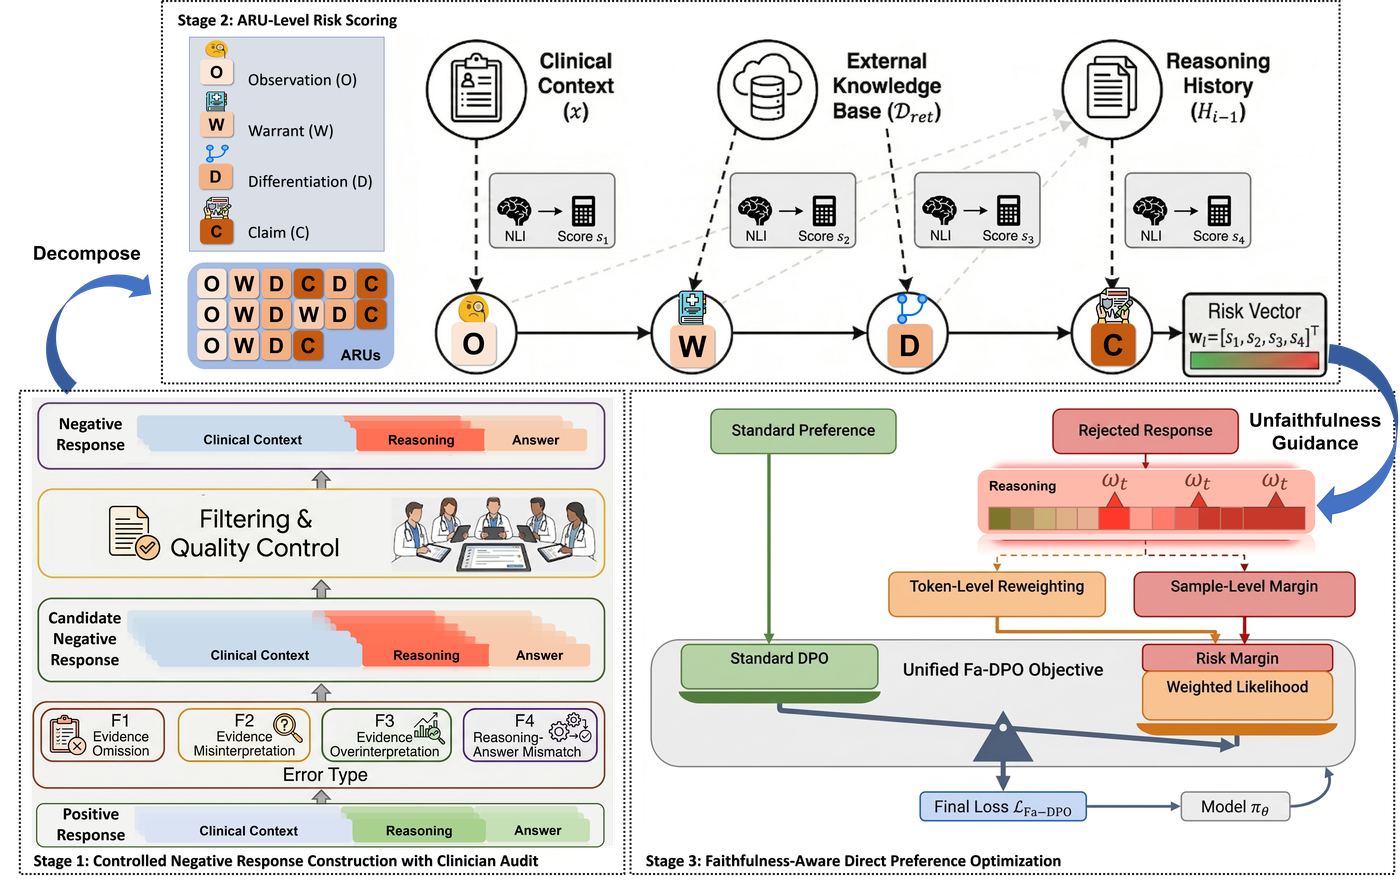
\includegraphics[width=1.0\linewidth]{overview.png}
\deleted{\textbf{Clinician-Audited Negative Response Construction:} we construct candidate negative responses through local rewriting under four controlled process-level failure types, apply automatic quality control, and validate a sampled subset with clinician audit.}
\deleted{\textbf{ARU-Level Faithfulness Risk Measurement:} we decompose each quality-controlled candidate negative response into ARUs, route the ARUs to reasoning-function-specific verification premises, and measure faithfulness risk.}
\deleted{faithfulness risk}
\deleted{risk}
    \caption[Fa-DPO framework overview.]{Overview of Fa-DPO. The framework proceeds in three stages. (1) \textbf{Controlled Negative Construction with Clinician Audit:} we construct candidate negative responses through local rewriting under four controlled process-level failure types, apply automatic quality control before risk-based retention, and validate a post-retention sample through clinician audit. (2) \textbf{ARU-Level Risk Scoring:} we decompose each quality-controlled candidate negative response into ARUs, route the ARUs to verifier-side, reasoning-function-specific verification premises, and compute ARU-level verification scores that estimate evidence-use risk for evidence-routed ARUs and reasoning--answer consistency risk for claim ARUs. (3) \textbf{Faithfulness-Aware Direct Preference Optimization:} we use the measured verification scores to retain high-risk candidates as rejected responses and parameterize the Fa-DPO objective. In each score vector, red denotes high risk, while green denotes low risk.}
    \label{fig:framework}
\end{figure*}

\subsection{Overview}
\label{sec:overview}

To align LLMs with faithful medical reasoning, we propose Fa-DPO, a faithfulness-aware DPO framework.
As shown in Figure~\ref{fig:framework}, our approach proceeds through three stages.

(1) \deleted{Clinician-Audited Negative Response Construction}\added{Offline Controlled Negative Construction with Clinician Audit}\revtag{R1.7,R3.6} (Sec.~\ref{sec:cot}):
We construct candidate negative responses \added{offline}\revtag{R3.6} through local rewriting under four controlled \deleted{faithfulness}\added{process-level}\revtag{R1.1} failure types, \deleted{apply automatic quality control to form the candidate pool for risk measurement, and use clinician audit to validate a sampled subset}\added{apply automatic quality control before risk measurement and retention, and use a post-retention clinician audit only to validate sampled retained negatives}\revtag{R1.7}.

(2) \deleted{ARU-Level Faithfulness Risk Measurement}\added{ARU-Level Risk Scoring}\revtag{R1.1} (Sec.~\ref{sec:graph}):
To provide fine-grained \deleted{faithfulness risk}\added{risk-scoring}\revtag{R1.1} signals for downstream DPO training, we decompose each quality-controlled candidate negative response into ARUs and assign each ARU a \deleted{faithfulness risk}\added{verifier-derived}\revtag{R1.1} score through multi-source evidence routing and NLI-based verification. \added{For evidence-routed ARUs, the score estimates evidence-use risk; for claim ARUs, including the final-answer claim, it estimates reasoning--answer consistency risk.}\revtag{R1.1}


(3) Faithfulness-Aware Direct Preference Optimization (Sec.~\ref{sec:dpo}):
To make DPO faithfulness-aware, we use the measured \deleted{faithfulness risk}\added{verification}\revtag{R1.1} scores as training signals to weight rejected-response log-ratios and set risk-adaptive preference margins.


\deleted{faithfulness risk}
\deleted{risk-scored}
\added{The raw candidate negative responses generated in Sec.~\ref{sec:cot} provide the foundational data for model training.}
\added{They are first filtered into a quality-controlled candidate pool and are then evaluated in Sec.~\ref{sec:graph} to attach ARU-level verification scores as fine-grained risk attributes.}
\added{The resulting risk-scored pool is filtered in Sec.~\ref{sec:dpo}; only the retained high-risk candidates serve as rejected responses and form DPO preference pairs.}


\subsection{\deleted{Controlled Negative Response Construction with Clinician Audit}\added{Offline Controlled Negative Construction with Clinician Audit}\revtag{R3.6}}
\label{sec:cot}
\deleted{Section title: Clinician-Audited Negative Response Construction}

To provide effective preference pairs for faithfulness-aware DPO, we construct candidate negative responses \added{offline}\revtag{R3.6} by introducing controlled \deleted{faithfulness}\added{process-level}\revtag{R1.1} failures in clinical reasoning, \deleted{automatically filter them into a quality-controlled candidate pool, and validate a sampled subset with clinician audit}\added{apply automatic quality control before risk measurement and retention, and use a post-retention clinician audit only to validate sampled retained negatives}\revtag{R1.7}.
In safety-critical MQA, a response can be unreliable not only when its final answer is wrong, but also when its reasoning is unsupported by the retrieved evidence or inconsistent with its own answer.
Accordingly, we first define the failure types used to generate candidate negatives, and then describe how automatic quality control, clinician audit, and risk-based retention serve different roles in the data construction pipeline.
\subsubsection{\deleted{Controlled Negative Response Construction}\added{Offline Controlled Negative Construction}\revtag{R3.6}}


\begin{table*}[htbp]
    \centering
    \scriptsize
    \setlength{\tabcolsep}{4pt}
    \renewcommand{\arraystretch}{1.5}
    \caption{Four controlled process-level failure types along the $(x,G)\!\to\!c\!\to\!a$ chain, with perturbation definitions and clinical examples under a shared scenario.}
    \begin{tabular}{
        >{\raggedright\arraybackslash}p{0.15\linewidth}
        >{\raggedright\arraybackslash}p{0.24\linewidth}
        >{\raggedright\arraybackslash}p{0.23\linewidth}
        >{\raggedright\arraybackslash}p{0.24\linewidth}
        >{\centering\arraybackslash}p{0.06\linewidth}
    }
        \toprule
        \textbf{Error Type} & \textbf{Definition} & \textbf{Local Perturbation} & \textbf{Clinical Example} & \textbf{Symbol} \\
        \midrule

        \textbf{Evidence Omission} &
        Clinically important available evidence is omitted or mentioned without being substantively used in the reasoning chain. &
        Remove or demote one key positive, negative, or contradictory finding while leaving the surrounding reasoning chain intact. &
        Diagnosing acute heart failure from edema while failing to use a reported normal ejection fraction. &
        F1 \\

        \textbf{Evidence Misinterpretation} &
        Available evidence is used, but its clinical meaning is interpreted incorrectly. &
        Preserve the cited evidence but alter its interpretation by shifting its threshold, temporal meaning, or pathophysiologic implication. &
        Interpreting a BNP of 90 pg/mL as definitive support for acute heart failure. &
        F2 \\

        \textbf{Evidence Overinterpretation} &
        Available evidence is interpreted too strongly, leading the reasoning chain to draw conclusions not warranted by the available degree of support. &
        Preserve the cited evidence but overstate its evidential strength, turning a limited or suggestive signal into decisive support. &
        Claiming that edema and mild dyspnea definitively establish cardiogenic pulmonary edema without sufficient imaging or biomarker support. &
        F3 \\

        \textbf{Reasoning--Answer Mismatch} &
        The final answer is not sufficiently supported by the preceding reasoning chain or is inconsistent with it. &
        Preserve the original final answer in the large majority of cases, but rewrite the late reasoning so that the answer is no longer entailed. &
        The reasoning argues against acute heart failure, but the final answer still states acute decompensated heart failure. &
        F4 \\
        \bottomrule
    \end{tabular}
    \label{tab:error_types}
\end{table*}

To support faithfulness-aware preference alignment in clinical reasoning, we construct candidate negative responses by introducing controlled \deleted{faithfulness}\added{process-level}\revtag{R1.1} failures into positive responses.
Table~\ref{tab:error_types} defines four localized \deleted{faithfulness}\added{process-level}\revtag{R1.1} failure types along the evidence-to-reasoning-to-answer chain. \deleted{F1--F3 target the evidence-to-reasoning interface, while F4 targets the reasoning-to-answer interface.}\added{F1--F3 are evidence-use faithfulness failures at the evidence-to-reasoning interface}\revtag{R1.1} $(x,G)\rightarrow c$\added{, including evidence omission, evidence misinterpretation, and overinterpretation. F4 is a reasoning-answer consistency failure at the reasoning-to-answer interface}\revtag{R1.1} $c\rightarrow a$\added{, where the final answer is not supported by, or conflicts with, the preceding reasoning process.}\revtag{R1.1} We use these types as an operational taxonomy for training-data construction rather than a complete taxonomy of natural clinical errors.

Starting from 13,092 positive responses in the MedCaseReasoning~\cite{wu2025medcasereasoning} training split, we construct candidate negatives by rewriting only a local span of each positive response $y_w = c^{+} \oplus a^{+}$ under a target type $e \in \mathcal{E} = \{\text{F1}, \text{F2}, \text{F3}, \text{F4}\}$. This produces an initial set of 52,368 raw negative candidates, corresponding to one attempted rewrite for each source positive and each controlled failure type. \added{This is an offline negative-construction stage: the generator may use retrieved evidence $G$ to construct rejected-response candidates with controlled evidence-use failures, but this does not mean that the final trained policy receives retrieved evidence at benchmark inference.}\revtag{R3.6} Let $\mathcal{M}$ denote the generator model, and let $P_{\mathcal{M}}(\cdot \mid x, G, y_w, e)$ denote the conditional distribution over rewritten responses given the input context, retrieved evidence, source positive response, and target failure type:
\begin{equation}
\tilde{y}_l \sim P_{\mathcal{M}}(\cdot \mid x, G, y_w, e)
\end{equation}
The sampled output $\tilde{y}_l$ is a candidate negative response rather than a final DPO rejected response. Each candidate negative response $\tilde{y}_l=c^{-}\oplus a^{-}$ preserves the case topic, answer style, and most of the reasoning trace while introducing one dominant \deleted{faithfulness}\added{process-level}\revtag{R1.1} failure. For F1--F3, \deleted{we keep the final answer unchanged to construct correct-answer, wrong-reasoning negatives}\added{we intentionally keep the final answer unchanged to construct correct-answer, wrong-reasoning negatives. This removes final-answer correctness as the distinguishing feature between the preferred and rejected responses and concentrates the preference contrast on evidence-use failures in the reasoning trace}\revtag{R2.8}. For F4, the answer is usually preserved, with a small predefined minority allowing answer changes to cover explicit reasoning--answer mismatch.

\added{These constructed negatives should be interpreted as controlled counterfactuals rather than as a complete model-error distribution. Local rewriting gives us control over the dominant failure type and keeps the clinical case, answer style, and most surrounding reasoning fixed, which helps isolate localized evidence-use and reasoning-answer consistency failures for preference learning. This preservation constraint improves controllability, but it does not by itself guarantee that the rejected responses follow the full distribution of naturally generated medical-LLM errors. We therefore describe F1--F4 as controlled evidence-use and reasoning-consistency failures in evidence-grounded MQA rather than as an exhaustive taxonomy of broader medical hallucination phenomena.}\revtag{R1.9}


\deleted{full prompt}
\added{In implementation, generation follows a plan--rewrite pipeline. One prompt decides whether the target error can be realized locally, which span should be edited, and whether the answer should be preserved. A second prompt applies the minimal rewrite. We then remove malformed or off-target outputs and apply judge-model quality control (QC) for realized type, single-error dominance, answer-policy compliance, and surface plausibility. This automatic quality-control stage accepts 47,393 candidates, accounting for 90.5\% of the raw candidates, which are then passed to the risk-measurement and rejected-response selection stages. Appendix~\ref{app:negative_protocol} gives the prompt structure and filtering details.}

\subsubsection{Clinician Audit of Constructed Negative Responses}

To \added{evaluate both the quality and the distributional limits of}\revtag{R1.9}\deleted{validate the quality of} the constructed negatives used for preference learning, we conduct a clinician audit on a stratified sample from the retained DPO negative pool. The audit checks whether the automatic pipeline realizes the intended local \deleted{faithfulness}\added{process-level}\revtag{R1.1} failure while preserving \added{contextual coherence,}\revtag{R1.9} clinical plausibility\added{, model-likeliness/naturalness of the injected error,}\revtag{R1.9} and the required answer policy.

Each audit item contains the case context, the original positive reasoning, the rewritten negative reasoning, and the target error type. Reviewers judge whether the rewrite realizes the intended local error, \added{whether one local error remains dominant, whether the full rewritten chain remains contextually coherent, whether the injected error is plausible as an error that a medical LLM could naturally produce,}\revtag{R1.9} whether the response remains clinically plausible, whether it follows the answer policy\added{, and whether it is acceptable as a controlled counterfactual negative}\revtag{R1.9}. The audit statistics and pool-level breakdown are reported in Sec.~\ref{subsec:negative_audit}, while detailed review instructions are \deleted{deferred to}\added{provided in}\revtag{R1.9} Appendix~\ref{app:negative_protocol}.


\subsection{\deleted{ARU-Level Faithfulness Risk Measurement}\added{ARU-Level Risk Scoring}\revtag{R1.1}}
\label{sec:graph}
To provide fine-grained \deleted{faithfulness}\added{verifier-derived}\revtag{R1.1} supervision for DPO, we \deleted{measure}\added{score}\revtag{R1.1} unit-level risk along the evidence-to-reasoning-to-answer chain. Sequence-level rejection labels indicate that a response is flawed, but they do not identify which reasoning units are \deleted{unfaithful}\added{unsupported, contradictory, or inconsistent with the final answer}\revtag{R1.1}. We therefore convert each quality-controlled candidate negative response into \deleted{function-aware}\added{reasoning-function-labeled}\revtag{R1.2} ARUs and verify each unit against its reasoning-function-specific evidence source. \added{For evidence-routed units, this risk concerns evidence use; for claim units, it concerns reasoning--answer consistency.}\revtag{R1.1}

\subsubsection{Atomic Reasoning Unit (ARU) Decomposition}
\label{sec:decomposition}
\deleted{To localize faithfulness risk before measurement, ARU decomposition converts each candidate negative response into minimal reasoning units. Given a candidate negative response $\tilde{y}_l = c^{-} \oplus a^{-}$, we segment the reasoning trace $c^{-}$ into Atomic Reasoning Units (ARUs) and append the extracted final answer $a^{-}$ as a special claim ARU. This yields the ordered ARU sequence $\mathcal{V}(\tilde{y}_l) = (v_1, v_2, \dots, v_L)$, where $v_1, \dots, v_{L-1}$ are reasoning-derived ARUs and $v_L$ is the final-answer claim ARU. Appendix~\ref{app:aru_protocol} details the parser protocol, retry rules, and quality-control procedure.}\added{To localize verification before scoring, ARU decomposition operationalizes atomic-claim decomposition as a medical-reasoning unit for optimization. We formalize ARUs as reasoning-function-labeled atomic clinical reasoning claims. This definition inherits the atomic-claim decomposition principle, but is specialized for evidence-grounded medical reasoning and preference optimization. Each ARU specifies not only a minimal checkable claim, but also its clinical reasoning function, the evidence route against which it should be verified, the local evidence-support or reasoning-consistency score, and the token span to which this score is assigned in the Fa-DPO objective. Thus, an ARU is not merely a renamed atomic claim; it is an optimization-oriented unit used to connect local verification scores with the Fa-DPO objective. Given a candidate negative response $\tilde{y}_l = c^{-} \oplus a^{-}$, we segment the reasoning trace $c^{-}$ into ARUs and append the extracted final answer $a^{-}$ as a special claim ARU. This yields the ordered ARU sequence $\mathcal{V}(\tilde{y}_l) = (v_1, v_2, \dots, v_L)$, where $v_1, \dots, v_{L-1}$ are reasoning-derived ARUs and $v_L$ is the final-answer claim ARU. Appendix~\ref{app:aru_protocol} details the parser protocol, retry rules, and quality-control procedure.}\revtag{R1.1,R1.2}

We then assign a reasoning-function label to each reasoning-derived ARU and treat the final-answer claim ARU as a claim. Following the Toulmin argumentation model~\cite{toulmin1958uses}, which represents argumentation through functional elements such as claims, supporting grounds, warrants, and rebuttals, we use four reasoning-function labels adapted to medical reasoning:

\begin{itemize}
    \item \textbf{Observation ($O$):} Facts stated in the clinical context $x$ (e.g., symptoms, lab results, or history).
    \item \textbf{Warrant ($W$):} General medical knowledge that links observations to conclusions.
    \item \textbf{Differentiation ($D$):} Steps that rule out alternative diagnoses based on the case evidence.
    \item \textbf{Claim ($C$):} Intermediate or final clinical conclusions, including the extracted final answer.
\end{itemize}

\added{This reasoning-function-specific decomposition also differs from coarse reasoning steps: a step may mix observations, warrants, differential reasoning, and final claims, whereas ARUs separate these functions so that each unit can be verified against the appropriate evidence source.}\revtag{R1.2}
This stage converts an unstructured response into a typed ARU sequence for the measurement stage below.

\subsubsection{\deleted{Multi-Source ARU Faithfulness Measurement}\added{Multi-Source ARU Verification}\revtag{R1.1}}
\label{sec:verification}
\deleted{faithfulness risk}
\deleted{risk}
\deleted{unfaithfulness}
\deleted{risk}
\added{To make each ARU usable as fine-grained supervision, this stage maps a typed ARU to a scalar verification score. The input to the verifier is a reasoning-function-specific verification premise $p$ and an ARU hypothesis $v_i$; the output is a score $s_i \in [0,1]$, where larger values indicate stronger evidence of unsupported, contradictory, or internally inconsistent reasoning. For evidence-routed ARUs, the score measures evidence-support risk against the patient context and retrieved medical evidence. For claim ARUs, including the final-answer claim, the score estimates whether the claim or final answer follows from the preceding reasoning under the verifier-side NLI setup. Let $P_{\text{ent}}(p,v)$, $P_{\text{neu}}(p,v)$, and $P_{\text{con}}(p,v)$ denote the verifier-predicted entailment, neutral, and contradiction probabilities when premise $p$ is used to verify hypothesis $v$. The NLI direction is fixed by this verification setup. The primary verifier uses forward entailment from the routed premise to the ARU, $e_i^{\rightarrow}=P_{\text{ent}}(p_i,v_i)$, because it asks whether the generated reasoning unit is supported by available evidence or prior reasoning. The reverse probability $e_i^{\leftarrow}=P_{\text{ent}}(v_i,p_i)$ asks whether the generated unit entails the premise, which is a coverage or specificity diagnostic rather than an evidence-support signal. A concise clinical summary can be faithful without entailing every detail in a larger evidence span; therefore, reverse entailment is not used for candidate retention, token weighting, the response-level risk score, or the risk-adaptive margin. Appendix~\ref{app:reverse_entailment_diagnostic} defines this optional diagnostic without incorporating it into Fa-DPO training. The scores of all ARUs in a candidate negative response $\tilde{y}_l$ form the verification-score vector $\mathbf{s}(\tilde{y}_l)=[s_1,s_2,\dots,s_L]\in[0,1]^L$. We define four reasoning-function-specific scoring rules, each choosing the premise that matches the function of the ARU.}

(1) Warrant Measurement.
Warrant ARUs express general medical knowledge, so their support should come from retrieved medical evidence rather than only from the patient record. For each warrant ARU $v_i$, we retrieve the top-$K$ snippets from the external knowledge base and concatenate them into an evidence premise $G_i$. The warrant risk score is
\begin{equation}
\label{eq:knowledge_score}
    s_i = \max \Big( P_{\text{con}}(G_i, v_i),\; \lambda_{\text{sup}} \cdot P_{\text{neu}}(G_i, v_i) \Big),
\end{equation}
where $0 \le \lambda_{\text{sup}} \le 1$ is the down-weighting coefficient for unsupported warrants. The contradiction term captures warrants that conflict with retrieved evidence, while the neutral term assigns a weaker risk to warrants that are not explicitly supported.

(2) Differentiation Measurement.
Differentiation ARUs explain why alternative diagnoses are ruled out. This decision depends on both patient-specific findings and general medical knowledge. Given the clinical context $x$ and the retrieved evidence block $G_i$, we construct the combined differentiation premise $E_i^{D}=\mathrm{concat}(x,G_i)$ and compute
\begin{equation}
\label{eq:diff_score}
    s_i = \max \Big( P_{\text{con}}(E_i^{D}, v_i),\; \lambda_{\text{diff}} \cdot P_{\text{neu}}(E_i^{D}, v_i) \Big),
\end{equation}
where $0 \le \lambda_{\text{diff}} \le 1$ is the down-weighting coefficient for unsupported exclusions. The combined premise makes the score sensitive to exclusions that contradict either the case evidence or the retrieved medical evidence, while still treating mere lack of explicit support as a weaker signal than contradiction.

(3) Observation Measurement.
Observation ARUs describe patient-specific facts and should be grounded primarily in the clinical context $x$. We first verify each observation ARU $v_i$ against $x$. A neutral-dominant result means that the record does not support the observation, but it does not by itself prove contradiction. In that case, we trigger a fallback plausibility check against the row-level auxiliary evidence block $G_{\text{row}}^{O}$. The fallback gate is
\[
g_i^{O} = \mathbb{I}\!\left[P_{\text{neu}}(x, v_i) \ge \max\!\big(P_{\text{ent}}(x, v_i), P_{\text{con}}(x, v_i)\big)\right],
\]
where $g_i^{O}=1$ indicates that the context-side verifier output is neutral-dominant. The observation risk score is
\begin{equation}
\label{eq:record_score}
    s_i = \max \Big( P_{\text{con}}(x, v_i),\; \lambda_{\text{miss}} \cdot P_{\text{neu}}(x, v_i),\; g_i^{O} \cdot \lambda_{\text{hal}} \cdot P_{\text{con}}(G_{\text{row}}^{O}, v_i) \Big),
\end{equation}
where $0 \le \lambda_{\text{miss}}, \lambda_{\text{hal}} \le 1$ are down-weighting coefficients for missing patient evidence and fallback hallucination evidence. The three terms respectively capture explicit contradiction with the patient record, unsupported patient-specific additions, and implausible fabrications detected by the fallback check. The auxiliary check can increase the risk when the added observation is implausible, but it does not remove the missing-record penalty.

\deleted{reasoning--answer faithfulness}
\added{(4) Claim Measurement.}
\added{Claim ARUs express intermediate or final clinical conclusions, so their premise should be the reasoning already stated in the response. For $i>1$, we define the reasoning-history premise as $H_{i-1}=\mathrm{concat}(v_1,\dots,v_{i-1})$. For the final-answer claim ARU, this premise provides a verifier-side reasoning-answer consistency estimate rather than an evidence-faithfulness adjudication in the narrow sense. The claim risk score is}
\begin{equation}
\label{eq:logic_score}
    s_i = \max \Big( P_{\text{con}}(H_{i-1}, v_i),\; \lambda_{\text{log}} \cdot P_{\text{neu}}(H_{i-1}, v_i) \Big),
\end{equation}
where $0 \le \lambda_{\text{log}} \le 1$ is the down-weighting coefficient for unsupported reasoning jumps. The contradiction term penalizes conclusions that conflict with the preceding reasoning, while the neutral term penalizes claims that are not justified by the earlier ARUs. If a claim ARU appears first, we set $H_0=\varnothing$, skip the NLI call, and assign $s_i=\lambda_{\text{log}}$, treating the claim as unsupported rather than contradictory.

\deleted{faithfulness risk}
\deleted{The response-level summary of this vector determines}
\added{Applying the corresponding rule to each ARU yields the verification-score vector $\mathbf{s}(\tilde{y}_l)$, which is passed to the subsequent Fa-DPO stage (Sec.~\ref{sec:dpo}). The response-level summary of this vector combines evidence-support risk from evidence-routed ARUs and verifier-derived reasoning-answer inconsistency from claim ARUs. The summary determines which constructed negatives are retained, and the ARU-level scores later determine where the training signal is concentrated inside each rejected response. Because these scores are produced by a learned verifier rather than direct medical adjudication, we further validate the verifier and report held-out calibration diagnostics.}
\added{Appendix~\ref{app:retrieval_protocol} details the retrieval and verification-premise construction pipeline, and Appendix~\ref{app:nli_validation} reports the stratified annotation protocol and the corresponding held-out calibration diagnostics.}


\subsection{Faithfulness-Aware Direct Preference Optimization}

\label{sec:dpo}
To incorporate the \deleted{ARU-level faithfulness signal}\added{ARU-level verification scores}\revtag{R1.1} measured in Sec.~\ref{sec:verification} into preference alignment, we propose \textbf{Fa-DPO} (Faithfulness-Aware Direct Preference Optimization) for clinical reasoning.
Following the DPO notation in Sec.~\ref{sec:preliminaries}, Fa-DPO uses each positive response as the preferred response $y_w$ and pairs it with one or more retained constructed negative responses as rejected responses $y_l$ under the same input $x$.
Fa-DPO \deleted{integrates faithfulness risk into DPO through three linked mechanisms.}\added{uses one ARU-level verification score to guide DPO through three linked mechanisms. For evidence-routed ARUs, this score measures evidence-support risk; for claim ARUs, it measures whether the claim or final answer follows from the preceding reasoning.}\revtag{R1.1} First, \deleted{response-level faithfulness risk}\added{the response-level summary of the ARU-level verification scores}\revtag{R1.1} determines which constructed negatives are retained as rejected responses. Second, \deleted{ARU-level faithfulness risk weights}\added{the ARU-level verification scores weight}\revtag{R1.1} the rejected-response log-ratio toward high-risk spans. Third, \deleted{response-level risk}\added{the response-level summary score}\revtag{R1.1} sets a sample-level adaptive preference margin so that clinically dangerous negatives must be separated more strongly. Together, these mechanisms determine which negatives enter DPO training, where the suppressive signal is applied, and how large the preference gap should be.

\subsubsection{\deleted{Faithfulness-Risk-Based}\added{Verification-Score-Based}\revtag{R1.1} Rejected-Response Selection}
\label{sec:retention}

To determine which constructed negatives enter DPO as rejected responses, we need a response-level score that summarizes both the worst local failure and how broadly risk appears in the chain. For any response $y$ with \deleted{ARU-level faithfulness risk}\added{ARU-level verification}\revtag{R1.1} scores $(s_1,\dots,s_L)$, we compute three statistics:
\begin{equation}
\label{eq:severity_components}
r_{\text{peak}}(y)=\max_{1 \le i \le L} s_i, \quad
r_{\text{cov}}(y)=\frac{1}{L}\sum_{i=1}^{L}\mathbb{I}[s_i>\tau], \quad
r_{\text{mean}}(y)=\frac{1}{L}\sum_{i=1}^{L} s_i,
\end{equation}
where $\tau$ is the ARU-level high-risk threshold used both for coverage aggregation and for the token mask below. Here, $r_{\text{peak}}$ captures the most severe local \deleted{faithfulness}\added{faithfulness or consistency}\revtag{R1.1} failure, $r_{\text{cov}}$ captures how many ARUs cross the high-risk threshold, and $r_{\text{mean}}$ captures the overall risk density of the response. We then combine these complementary signals into a raw severity score:
\begin{equation}
\label{eq:severity_raw}
S_{\text{raw}}(y)=\omega_{\text{peak}} \, r_{\text{peak}}(y)+\omega_{\text{cov}} \, r_{\text{cov}}(y)+\omega_{\text{mean}} \, r_{\text{mean}}(y),
\end{equation}
where $\omega_{\text{peak}}$, $\omega_{\text{cov}}$, and $\omega_{\text{mean}}$ are nonnegative aggregation weights and $\omega_{\text{peak}}+\omega_{\text{cov}}+\omega_{\text{mean}}>0$. Larger weights make the response-level score more sensitive to the corresponding failure pattern. Finally, we normalize the raw score to obtain the response-level \deleted{faithfulness risk}\added{verification score}\revtag{R1.1}:
\begin{equation}
\label{eq:faithfulness_risk_score}
R(y)=\frac{S_{\text{raw}}(y)}{\omega_{\text{peak}}+\omega_{\text{cov}}+\omega_{\text{mean}}}, \quad R(y)\in [0,1],
\end{equation}
where the range follows from $r_{\text{peak}}(y),r_{\text{cov}}(y),r_{\text{mean}}(y)\in[0,1]$. This scalar score is used only to rank and retain candidate negatives at the response level; the original ARU scores remain available for token-level weighting below. The concrete coefficient values are given in Appendix~\ref{app:training_details}.

For DPO training, we retain a candidate negative response $\tilde{y}_l$ as a rejected response if $R(\tilde{y}_l)\ge \gamma$, where $\gamma$ is the retention threshold. \added{This threshold is fixed before the final clinician audit, and the audit results are not fed back into the retention rule.}\revtag{R1.7} For each source positive response $y_w$ with at least one quality-controlled candidate, we keep all paired candidates that satisfy this threshold; if none does, we keep only the paired candidate with the largest $R(\tilde{y}_l)$ so that each covered preferred response remains paired with at least one rejected response. The retained tuples form the Fa-DPO training set $\mathcal{D}_{\text{Fa}}=\{(x,y_w,y_l,\mathbf{s}_l)\}$, where $y_l$ denotes a retained rejected response and $\mathbf{s}_l=\mathbf{s}(y_l)$. In the reported construction, this risk-based selection yields 34,204 retained rejected responses, or 72.2\% of the quality-controlled candidates, from 12,411 source positives. Since each retained rejected response is paired with its corresponding preferred response, the final DPO training set contains 34,204 preference pairs. The concrete threshold is given in Appendix~\ref{app:training_details}.

\deleted{ARU-Risk-Guided}
\subsubsection{ARU-Risk-Guided Rejected-Response Weighting in DPO}
\label{sec:token_reweighting}

To prevent DPO from treating correct and erroneous spans equally inside a rejected response, we use \deleted{ARU-level faithfulness risk}\added{ARU-level verification scores}\revtag{R1.1} to reweight the rejected-response log-ratio. Clinical reasoning errors are often confined to a few spans within an otherwise plausible reasoning chain, but standard DPO applies one sequence-level rejected signal to the whole negative response. We therefore map \deleted{ARU-level faithfulness risk}\added{ARU-level verification scores}\revtag{R1.1} to token weights and make the rejected-side DPO term more sensitive to spans most likely to be \deleted{unfaithful}\added{unsupported, contradictory, or inconsistent}\revtag{R1.1}.

For a retained rejected response $y_l$ with \deleted{risk}\added{verification-score}\revtag{R1.1} vector $\mathbf{s}_l=[s_1,\dots,s_L]$, we first map \deleted{ARU-level faithfulness risk}\added{ARU-level verification}\revtag{R1.1} scores to the token level. Let $\operatorname{tok}(y_l) = \big(z^{(l)}_1, z^{(l)}_2, \dots, z^{(l)}_{T_l}\big)$ denote the tokenized rejected response, and let $\mathcal{T}(v_i) \subseteq \{1, \dots, T_l\}$ denote the set of token indices belonging to the ARU $v_i$. The extracted final answer tokens belong to the final-answer claim ARU $v_L$. Before applying the mask, we enforce a non-overlapping ARU partition: overlaps between reasoning-derived ARUs are resolved in favor of the earlier span in the serialized order, and any residual overlap between the rationale and the extracted final answer is assigned to $v_L$. We then define the token reweighting mask:
\begin{equation}
\label{eq:topology_mask}
m_t =
\begin{cases}
\deleted{\alpha}\added{1+\alpha s_i}\revtag{R1.4}, & \text{if } t \in \mathcal{T}(v_i) \text{ for some } i \text{ and } s_i > \tau \\
\epsilon, & \text{otherwise}
\end{cases},
\end{equation}
where \deleted{$\alpha > \epsilon > 0$}\added{$\alpha>0$ and $\epsilon>0$}\revtag{R1.4}. Tokens covered by ARUs above the shared high-risk threshold $\tau$ receive \deleted{weight $\alpha$}\added{a continuous risk-scaled weight}\revtag{R1.4}, and all other tokens receive \deleted{weight}\added{the background weight}\revtag{R1.4} $\epsilon$. \added{Because $s_i\in[0,1]$, the raw token weights satisfy $m_t\in[\epsilon,1+\alpha]$.}\revtag{R1.4}

We then replace the rejected-response sequence log-ratio in DPO with a normalized token-weighted rejected log-ratio:
\begin{equation}
\label{eq:weighted_rejected_logratio}
\Delta_m(x,y_l,\mathbf{s}_l)
=
\frac{T_l}{\sum_{t=1}^{T_l} m_t}
\sum_{t=1}^{T_l}
m_t
\Big[
\log \pi_\theta(z^{(l)}_t \mid x, z^{(l)}_{<t})
-
\log \pi_{\text{ref}}(z^{(l)}_t \mid x, z^{(l)}_{<t})
\Big].
\end{equation}
Here, $z^{(l)}_{<t}$ denotes the preceding tokens in the tokenized rejected response, and the subscript $m$ indicates that the rejected log-ratio is computed under the token mask $m_t$. \added{The bracketed token-level ratio is computed in the same policy-over-reference direction as $\rho_\theta(x,y)$. Because $\rho_\theta(x,y)$ uses unnormalized autoregressive sequence log-probabilities, Eq.~\ref{eq:weighted_rejected_logratio} is kept on the same token-sum scale.}\revtag{R1.3,R1.4} \deleted{The factor $T_l/\sum_t m_t$ keeps the scale comparable to the unweighted sequence log-ratio, while the mask increases the contribution of high-risk spans.}\added{Equivalently, Eq.~\ref{eq:weighted_rejected_logratio} uses the normalized effective token weight $\omega_t=T_lm_t/\sum_{j=1}^{T_l}m_j$. These weights satisfy $\sum_{t=1}^{T_l}\omega_t=T_l$ and $\omega_i/\omega_j=m_i/m_j$ within the same rejected response. Thus, the normalization preserves the same total effective token mass as the unweighted rejected-response sequence log-ratio, while preserving the relative emphasis introduced by the ARU-risk mask. In the uniform case $m_t=c$ for all tokens, $\omega_t=1$ and the expression reduces exactly to the standard rejected-response sequence log-ratio. The normalization is therefore a local credit-assignment device: it redistributes a fixed rejected-side token mass toward high-risk spans, rather than increasing the total token mass of the rejected response. Sparse high-risk masks can increase the relative weight of individual high-risk tokens, but because $m_t\in[\epsilon,1+\alpha]$, the normalized effective token weight is bounded by $\omega_t\le (1+\alpha)/\epsilon$; therefore, the weighting cannot produce unbounded effective token weights. This fixed-mass property is a statement about rejected-side token weights, not a guarantee that gradient norms are constant, because log-probability gradients still depend on the token distribution, model confidence, and current parameters.}\revtag{R1.4} \added{Appendix~\ref{app:normalization_stability} therefore empirically tests this normalization against uniform, unnormalized, and capped variants.}\revtag{R2.9} When Fa-DPO minimizes the final objective below, lowering this weighted rejected log-ratio increases the preference gap mainly through tokens aligned to high-risk ARUs.

\subsubsection{Sample-Level Risk-Adaptive Preference Margin in DPO}
\label{sec:sample_margin}
To require a larger preference gap for clinically riskier rejected responses, we introduce a sample-level risk-adaptive preference margin in DPO in addition to the token weighting above. \deleted{Standard DPO uses the same margin for every sample, whereas our margin increases with the overall severity of the retained negative response.}\added{Standard DPO uses no explicit sample-dependent additive margin, whereas Fa-DPO introduces a bounded risk-dependent margin for the rejected response.}\revtag{R1.5} Using the normalized response-level risk score above, we map $R(y_l)$ to an additive training margin:
\begin{equation}
\label{eq:severity_margin}
\delta(y_l)=\eta \cdot \min \big( \kappa_{\delta} \, R(y_l), \, c_{\text{sat}} \big),
\end{equation}
where $\kappa_{\delta}$ controls the linear growth rate before saturation, $c_{\text{sat}}$ sets the saturation point, and $\eta$ rescales the capped severity signal. The concrete values are given in Appendix~\ref{app:training_details}. This bounded mapping increases the margin for riskier negatives while preventing a few extreme cases from dominating the preference logit.
\added{Because $R(y_l)\in[0,1]$ and $\eta,\kappa_{\delta},c_{\text{sat}}>0$, $\delta(y_l)$ is monotone non-decreasing in rejected-response risk: if $R(y_l^{(1)})\le R(y_l^{(2)})$, then $\delta(y_l^{(1)})\le\delta(y_l^{(2)})$. The mapping is linear before saturation and constant after saturation, so it does not reverse the risk ordering, although high-risk negatives may share the same capped margin. It is bounded by $0\le\delta(y_l)\le\eta c_{\text{sat}}$.}\revtag{R1.5}

We then subtract $\delta(y_l)$ from the DPO logit, so that the model must prefer the positive response $y_w$ to a higher-risk negative response $y_l$ by a larger margin.
\added{The margin should be interpreted as a pairwise large-margin offset in the empirical DPO logit, not as a new global response-level reward. A higher value of $\delta(y_l)$ lowers the logit for a preference pair and therefore requires a larger preferred-minus-rejected score gap for that rejected response. Thus, the margin preserves monotonicity of the required preference separation, not necessarily monotonicity of a global reward ranking over all possible responses.}\revtag{R1.5}

\subsubsection{Unified Fa-DPO Objective}

We combine the sample-level risk-adaptive preference margin and the token-weighted rejected log-ratio into the final Fa-DPO objective:

\begin{equation}
\label{eq:fa_dpo}
\begin{split}
\mathcal{L}_{\text{Fa-DPO}}(\pi_\theta; \pi_{\text{ref}})
&= -\mathbb{E}_{(x, y_w, y_l, \mathbf{s}_l) \sim \mathcal{D}_{\text{Fa}}} \Bigg[
\log \sigma \Bigg(
{\color{blue}\beta \rho_\theta(x,y_w)}
- \beta \Delta_m(x,y_l,\mathbf{s}_l)
- \delta(y_l)
\Bigg) \Bigg],
\end{split}
\end{equation}

where $\delta(y_l)$ denotes the sample-level risk-adaptive margin defined in Eq.~\ref{eq:severity_margin},
$\Delta_m(x,y_l,\mathbf{s}_l)$ denotes the token-weighted rejected log-ratio defined in Eq.~\ref{eq:weighted_rejected_logratio},
and $\beta$ is the temperature parameter that controls the deviation from the reference model.

\deleted{The preferred-response log-ratio increases the relative probability of $y_w$. The weighted rejected log-ratio enters the preference logit with a negative sign, so lowering it enlarges the gap against $y_l$, with larger influence on high-risk spans through $m_t$.}
\deleted{faithfulness risk signal}
\added{Both $\rho_\theta(x,y_w)$ and $\Delta_m(x,y_l,\mathbf{s}_l)$ are computed in the policy-over-reference direction. Therefore, minimizing the loss increases the preferred-response log-ratio while decreasing the rejected-response log-ratio, with the rejected-side decrease concentrated on high-risk spans through $m_t$. The margin term further requires a larger preference gap for riskier negatives. Thus, the same ARU-level verification scores first select useful negatives, then determine where and how strongly the final DPO objective separates them from the preferred response.}
\added{This objective remains tied to standard DPO through the policy-over-reference log-ratio. In standard DPO, the implicit reward can be written as $r_\theta(x,y)=\beta\rho_\theta(x,y)+C(x)$, where $C(x)$ cancels in pairwise differences. Fa-DPO keeps this log-ratio basis but modifies the empirical pairwise logit by using a normalized token-weighted rejected term and a bounded rejected-side margin. We therefore view Fa-DPO as a bounded large-margin variant of DPO rather than an unmodified standard DPO objective or a new closed-form reward-model derivation. Under the usual KL-regularized policy form}
\begingroup
\color{blue}
\[
\pi_r^*(y|x)=
\frac{\pi_{\mathrm{ref}}(y|x)\exp(r(x,y)/\beta)}
{Z_r(x)},
\qquad
Z_r(x)=\sum_y \pi_{\mathrm{ref}}(y|x)\exp(r(x,y)/\beta),
\]
\endgroup
\added{normalizability depends on finite reward scale and the support of the reference policy. Fa-DPO's additive margin is finite, pair-dependent, and does not change the support of $\pi_{\mathrm{ref}}$; therefore, the margin does not by itself introduce an unbounded reward-scale or support-mismatch problem. We make this boundedness claim for the empirical large-margin objective, not as a proof that Fa-DPO preserves the standard DPO optimal-policy theorem unchanged.}\revtag{R1.5}

\section{Experiments}
\label{sec:experiments}

\deleted{We evaluate Fa-DPO from five complementary perspectives: shared experimental settings, main empirical results, controlled ablations, analysis of faithfulness gains, and validation of evidence reliability. This structure separates how the method is evaluated, whether it improves reasoning faithfulness and end-task performance, which components contribute to the gains, where those gains arise in the reasoning chain, and how reliable the supporting evidence is.}\added{The experiments are organized as a connected evidence chain. We first establish matched evaluation conditions, then test whether Fa-DPO improves automatic process metrics and final-answer accuracy, check whether simpler faithfulness-oriented alternatives can explain the gains, identify the components and hyperparameters that support the effect, locate the changes inside the reasoning chain, and finally validate the evidence sources on which these claims rely.}

\subsection{Experimental Settings}
\label{subsec:settings}

\deleted{This subsection describes the common evaluation framework used throughout the experiments. We first introduce the datasets, baselines, and metrics, and then summarize the implementation details needed to interpret the later comparisons under matched and reproducible conditions.}\added{This subsection sets the common ground for all later comparisons. The datasets define where training, answer-accuracy evaluation, and process analysis occur; the baselines define what Fa-DPO is compared against; the metrics define what each claim measures; and the implementation and statistical protocols define how differences are attributed under matched conditions.}

\subsubsection{Datasets}
\label{subsubsec:datasets}
We use one constructed preference dataset for alignment training, four multiple-choice benchmark settings for final-answer accuracy, and the MedCaseReasoning~\cite{wu2025medcasereasoning} test split for controlled \deleted{process-faithfulness}\added{process-metric}\revtag{R1.1} analysis\deleted{, and one supplementary external pilot set for natural-error coverage}\revtag{R1.17,R2.2,R2.6}. All compared models use fixed evaluation splits; the appendix protocols \deleted{and release artifacts}\added{record}\revtag{R1.6} the split identities, benchmark versions, and retained subset sizes.

For preference training, we construct \added{controlled counterfactual}\revtag{R1.9} pairs from the MedCaseReasoning training split, whose long diagnostic rationales allow local perturbation of intermediate reasoning while keeping the clinical case fixed. Each retained instance is represented as $(x, y_w, y_l, \mathbf{s}_l)$, where $y_w$ is the preferred reasoning-and-answer response, $y_l$ is a locally rewritten rejected response with a controlled F1--F4 \deleted{faithfulness}\added{process-level}\revtag{R1.1} failure, and $\mathbf{s}_l$ is the \deleted{ARU-level faithfulness risk}\added{ARU-level verification-score}\revtag{R1.1} vector for the rejected response. \added{Automatic construction and quality control yield 47,393 candidate pairs; ARU-score-based retention yields 34,204 final preference pairs from 12,411 source positives.}\revtag{R1.10} \deleted{Standard DPO and Fa-DPO}\added{Standard DPO-Retained-34K and Fa-DPO-Retained-34K}\revtag{R1.10} use the same retained pair content, while Fa-DPO additionally uses $\mathbf{s}_l$ for token-level weighting and the sample-level margin. The MedCaseReasoning test split is held out from preference-data construction and used only for reasoning analysis.

For final-answer accuracy, we evaluate MedQA~\cite{jin2021disease}, MedBullets-op4/op5~\cite{chen2025benchmarking}, and MedXpertQA~\cite{zuo2025medxpertqa}. These \deleted{exam-style}\added{task-aligned}\revtag{R1.17,R2.2,R2.6} MQA benchmarks test transfer to standard medical questions, distractor-rich exam settings, and harder multi-step clinical reasoning. \deleted{We further use a sampled Med-HALT reasoning pilot set as a supplementary external check of natural-error coverage.}\revtag{R1.17,R2.2,R2.6}

\added{The retained preference pool is controlled and risk-enriched rather than prevalence-preserving. All four F1--F4 failure types remain represented, but Appendix~\ref{app:dataset_bias_details} reports the retained-pool data card, retained/raw rates, local-rewrite naturalness audit, and bias-source table. We therefore use the retained pool as controlled supervision for evidence-use and reasoning-answer consistency failures, not as an unbiased natural-error sample.}\revtag{R4.3}

\subsubsection{Baselines}

\deleted{We organize the comparison systems into three categories and use them in two ways: controlled matched Fa-DPO vs.\ Standard DPO comparisons and a broader released-baseline comparison.}\added{We use three baseline layers. Released-model baselines contextualize competitiveness across general instruction, medical-adapted, and reasoning-oriented medical models; the complete released-model list is reported in Table~\ref{tab:competitiveness_reference}. Matched retained-pair DPO controls provide the primary causal comparison, and representative faithfulness-oriented controls test simpler explanations for the observed gain.}\revtag{R1.10,R2.4}

For the matched comparison, we select six 8B starting points spanning general-instruction, medical-adapted, and reasoning-enhanced regimes: Llama-3.1-8B-Instruct~\cite{dubey2024llama}, Qwen3-8B~\cite{yang2025qwen3}, their m23k-SFT variants~\cite{huang2025m1}, UltraMedical-3.1-8B~\cite{zhang2024ultramedical}, and II-Medical-8B~\cite{intelligentinternet2025iimedical8b}. For each starting point, we train one \deleted{Standard DPO variant and one Fa-DPO variant}\added{Standard DPO-Retained-34K variant and one Fa-DPO-Retained-34K variant}\revtag{R1.10}. Within each pair, the two variants share the same 34,204 retained preference pairs, preprocessing, train/dev split, training budget, verifier pipeline, prompt template, decoding setup, and answer extraction rule; the intended difference is only the preference objective.

\added{On the representative II-Medical-8B backbone, we additionally compare against SFT-faithful, Standard DPO-QC-All, Standard DPO-Random-34K, Standard DPO-Retained-34K, and verifier reranking with $K=4$ or $K=8$. These controls separate positive-only imitation, full-candidate DPO, sample-count effects, retained-pool effects, and inference-time verification. Appendix~\ref{app:faithfulness_baseline_protocol} gives the control protocol.}\revtag{R1.10,R2.4}

\subsubsection{Evaluation Metrics}
\label{subsubsec:eval_metrics}
We evaluate Fa-DPO with three groups of metrics: final-answer accuracy, \deleted{process faithfulness}\added{automatic process metrics}\revtag{R2.1,R2.5}, and ARU unfaithfulness shift by reasoning function. Final-answer accuracy is measured on multiple-choice benchmarks. The two process-level analyses use the parser-verifier pipeline introduced in Sec.~\ref{sec:decomposition} and Sec.~\ref{sec:verification}, where an LLM parser decomposes each response into typed ARUs, with the extracted final answer appended as a final-answer claim ARU, and an NLI-based verifier checks each ARU against its verification premise. Here, \emph{ARU} and \emph{verification premise} follow the definitions in those two sections. \deleted{These automatic process metrics provide mechanism-oriented proxy evidence rather than direct measures of absolute clinical correctness.}\added{Because these process metrics are computed by the same ARU parser and NLI verifier used to construct the Fa-DPO risk signal, they are interpreted as diagnostic indicators of evidence-use and consistency behavior rather than independent clinical ground truth or direct measures of absolute clinical correctness. The same-answer clinician audit in Appendix~\ref{app:same_answer_clinician_details} provides directional validation of these indicators, not a replacement for clinician-adjudicated evaluation.}\revtag{R2.1,R2.5}
\begin{itemize}[leftmargin=*]
    \item \textbf{Answer Accuracy.} We report Accuracy (\%) for each multiple-choice question (MCQ) dataset and the simple macro-average over MedQA~\cite{jin2021disease}, MedBullets-op4~\cite{chen2025benchmarking}, MedBullets-op5~\cite{chen2025benchmarking}, and MedXpertQA~\cite{zuo2025medxpertqa}. We keep MedBullets-op4~\cite{chen2025benchmarking} and MedBullets-op5~\cite{chen2025benchmarking} separate because they have different numbers of options and therefore different difficulty levels. This metric measures whether the model predicts the correct final answer.
\item \deleted{Process Faithfulness and Consistency}
\item \deleted{measure process faithfulness with four complementary metrics}
\item \deleted{report two groups of verifier-derived process metrics}
\item \deleted{Claim Inconsistency Rate}
    \item \added{\textbf{Automatic Process Metrics.} We report four ARU/NLI-based metrics, grouped by diagnostic role. The evidence-support metrics are \textbf{Support Rate}, the fraction of ARUs entailed by their verification premises, $\textit{Support Rate} = N_{\text{sup}} / N_{\text{ARU}}$, and \textbf{Unsupported Medical Reasoning Rate}, the fraction of warrant and differentiation ARUs unsupported by their verification premises, $\textit{Unsupported Medical Reasoning Rate} = N_{\text{unsup}}^{\text{WD}} / N_{\text{WD}}$. The latter is not the complement of Support Rate because it is computed only over clinically inferential warrant and differentiation units. The evidence-conflict metric is \textbf{Contradiction Rate}, the fraction of ARUs that contradict their verification premises, $\textit{Contradiction Rate} = N_{\text{contra}} / N_{\text{ARU}}$. The reasoning-answer consistency metric is \textbf{Reasoning-Answer Inconsistency Rate}, the verifier-labeled fraction of claim ARUs unsupported or contradicted by the preceding ARUs in the same response, $\textit{Reasoning-Answer Inconsistency Rate} = N_{\text{inc}}^{\text{C}} / N_{\text{C}}$. Here, $N_{\text{ARU}}$ is the total number of ARUs, $N_{\text{sup}}$ the number labeled as entailment, $N_{\text{contra}}$ the number labeled as contradiction, $N_{\text{WD}}$ the number of warrant and differentiation ARUs, $N_{\text{unsup}}^{\text{WD}}$ the number of such ARUs that are unsupported, $N_{\text{C}}$ the number of claim ARUs including the final-answer claim ARU, and $N_{\text{inc}}^{\text{C}}$ the number of verifier-labeled inconsistent claim ARUs.}
    \item \textbf{ARU-Level Unfaithfulness Shift.} We also report the change in the non-entailment rate for each reasoning function as a descriptive before/after analysis. This analysis shows whether the effect is broad-based across observation, warrant, differentiation, and claim ARUs. Appendix~\ref{app:process_metrics} gives the full subset-construction and computation protocol.
\end{itemize}

\deleted{Together, these metrics connect the paper's claims to evidence at three levels: final-answer correctness, verifier-derived reasoning support and consistency, and the location of unfaithful steps inside the reasoning chain.}
\added{Together, these metrics connect the paper's claims to evidence at three levels: final-answer correctness, verifier-derived indicators of reasoning support and consistency, and the location of unfaithful steps inside the reasoning chain.}

\subsubsection{Implementation Details}
\added{These implementation details ensure that the matched comparisons differ in the intended training objective rather than in compute, decoding, or verifier-side processing.}

We run both \deleted{Standard DPO and Fa-DPO}\added{Standard DPO-Retained-34K and Fa-DPO-Retained-34K}\revtag{R1.10} on each of the six 8B base models using 8 NVIDIA A100 GPUs. Across the matched comparisons, the two variants share the same training budget and core optimization setup: one training epoch, learning rate $5\times10^{-7}$ with cosine decay and warmup ratio 0.1, effective batch size 32 preference pairs under bf16, maximum sequence length 4096, and LoRA-based parameter-efficient tuning. Fa-DPO further uses fixed token-level and sample-level risk coefficients chosen in preliminary development experiments; Appendix~\ref{app:training_details} reports the full training coefficients and run-time defaults.

\deleted{Standard DPO variant}
\deleted{Fa-DPO counterpart}
\deleted{DeBERTa-v3-large-mnli-fever-anli-ling-wanli}
\added{For the pairwise comparisons in Table~\ref{tab:matched_main_results}, each Standard DPO-Retained-34K variant uses the same base model, preference source, preprocessing pipeline, train/dev split, training budget, verifier-side retrieval pipeline, prompt template, decoding configuration, and answer extraction rule as its Fa-DPO-Retained-34K counterpart, differing only in the preference objective. Benchmark evaluation uses the final checkpoint from the single training epoch rather than dev-set model selection. All main-text mechanism analyses use the II-Medical-8B~\cite{intelligentinternet2025iimedical8b} matched pair with the same retrieval pipeline and the public DeBERTa-v3-large NLI checkpoint\footnote{Hugging Face model page \url{https://huggingface.co/MoritzLaurer/DeBERTa-v3-large-mnli-fever-anli-ling-wanli}.}~\cite{he2023debertav3,laurer2023less}. Appendix~\ref{app:training_details} and Appendix~\ref{app:retrieval_protocol} document the corresponding training and routed-premise protocols.}

\added{Thus, the implementation protocol keeps optimization, inference, and verifier inputs aligned across each matched pair, making later process and accuracy differences interpretable as objective-level effects.}

\subsubsection{\added{Statistical Analysis}\revtag{R1.13,R2.10}}
\added{All comparisons between Standard DPO-Retained-34K and Fa-DPO-Retained-34K are paired because both systems are evaluated on the same questions under matched decoding, answer extraction, and verifier-side processing. For same-answer process metrics, each retained case contributes one response-level metric per system. We report case-weighted means and paired deltas, with 95\% confidence intervals from 10,000 paired cluster-bootstrap replicates over cases. Each bootstrap sample keeps both system responses and all nested ARUs from the sampled cases together; ARU counts are reported as measurement denominators, not as independent resampling units.}\revtag{R1.13,R2.10}

\added{For downstream accuracy, macro-average uncertainty is estimated with benchmark-stratified paired bootstrap confidence intervals. Each replicate resamples paired test questions within each benchmark, recomputes the four benchmark accuracies, and then recomputes the simple four-benchmark macro-average. Benchmark-level paired tests, Holm-adjusted p-value screening, and the six-backbone Wilcoxon direction summary are reported as supplementary diagnostics; the main text emphasizes paired deltas and confidence intervals, and the 1.2--1.6 point range denotes the observed cross-backbone range rather than an uncertainty interval.}\revtag{R1.13}

\added{For representative ablation analyses, we use the same paired question-level bootstrap protocol for macro-average drops and apply Holm adjustment within the leave-one-out family. Detailed drop-difference checks for closely spaced components are reported with the appendix ablation analyses.}\revtag{R1.14}

\deleted{Together, these choices define a matched evaluation protocol in which the reported differences can be attributed to the training objective and analysis design rather than to changes in data, decoding, or compute.}\added{Together, these statistical choices keep the main-text uncertainty reporting focused on paired effect estimates while leaving detailed p-value screening to the supplementary analyses.}

\subsection{Main Results}
\label{subsec:main_results}
\deleted{We first report matched process-faithfulness results on same-answer subsets, then matched answer-accuracy results on four MQA benchmarks, and finally compare the strongest Fa-DPO variant with released baselines to test whether the gains remain competitive beyond the paired setting.}
\added{We next evaluate whether Fa-DPO improves verifier-derived process indicators and final-answer performance. Because these process metrics are computed by the ARU/NLI verifier used in our training pipeline, we interpret them as diagnostic indicators of evidence-use and claim-consistency behavior rather than independent ground-truth labels. The results are organized as a progression: first, same-answer process-metric comparisons test whether these indicators improve when final-answer correctness is fixed; second, matched benchmark results test whether these process gains coincide with better answer accuracy; third, released-baseline comparisons test broader competitiveness; and fourth, faithfulness-oriented controls test whether simpler alternatives explain the representative gains.}

\subsubsection{\deleted{Process-Faithfulness Results}\added{Automatic Process Metrics}\revtag{R1.1,R2.1}}
\deleted{process-faithfulness metrics}
\deleted{The main text reports paired deltas only, while detailed subset-construction rules and the representative detailed table are deferred to Appendix~\ref{app:process_metrics}.}
\added{We first evaluate whether Fa-DPO improves the automatic process indicators when final-answer correctness is held fixed. For each paired comparison, we construct a same-answer subset from the MedCaseReasoning~\cite{wu2025medcasereasoning} test split by keeping only questions on which both compared models predict the correct final answer, and then compute the four automatic ARU/NLI-based process metrics introduced in Sec.~\ref{subsubsec:eval_metrics}. This same-answer control focuses the comparison on process indicators rather than answer accuracy, but it is a conditional mechanism analysis rather than an unconditional estimate of full-test response quality. The same-answer table reports paired deltas with paired uncertainty; full-test and correctness-stratified checks are reported below and in Appendix~\ref{app:process_metrics}.}

\begin{table*}[htbp]
    \centering
    \scriptsize
    \renewcommand{\arraystretch}{1.12}
    \setlength{\tabcolsep}{3pt}
    \caption[\deleted{Process-faithfulness results}\added{Automatic process metrics}\revtag{R1.1,R2.1} across six paired base models.]{\deleted{Process-faithfulness results}\added{Automatic process metrics}\revtag{R1.1,R2.1} across six paired base models on MedCaseReasoning same-answer subsets. We report question-level mean paired differences ($\Delta$ $=$ \textit{\deleted{Fa-DPO}\added{Fa-DPO-Retained-34K}\revtag{R1.10}} $-$ \textit{\deleted{Standard DPO}\added{Standard DPO-Retained-34K}\revtag{R1.10}}) for four \added{automatic ARU/NLI-based}\revtag{R2.1} process metrics\added{, with paired cluster-bootstrap 95\% confidence intervals over retained cases}\revtag{R1.13,R2.10}. \deleted{\textit{Support Rate}, \textit{Contradiction Rate}, and \textit{Unsupported Medical Reasoning Rate} are evidence-faithfulness proxy metrics, while \textit{Claim Inconsistency Rate} is a reasoning-answer consistency metric.}\added{The metrics are ordered by conceptual group: \textit{Support Rate} and \textit{Unsupported Medical Reasoning Rate} are evidence-support indicators, \textit{Contradiction Rate} is an evidence-conflict indicator, and \textit{Reasoning-Answer Inconsistency Rate} is a reasoning-answer consistency metric.}\revtag{R1.1,R2.1,R3.8} Positive values are better for \textit{Support Rate}, while negative values are better for the other three metrics. \deleted{Here, $n$ denotes the retained subset size for each pair.}\added{Here, $n$ denotes retained same-answer cases, responses denotes $2n$, and ARUs $N$ is the total ARU measurement count, not the resampling unit. Supplementary multiplicity-adjusted p-value screening is reported in Appendix~\ref{app:process_metrics}.}\revtag{R1.13,R2.10}}
    \label{tab:paired_process_summary}
    \begin{adjustbox}{max width=\textwidth}
    \begingroup\color{blue}
    \begin{tabular}{llrrrllll}
    \toprule
    \textbf{Category} & \textbf{Model} & \textbf{$n$} & \textbf{Resp.} & \textbf{ARUs $N$} & \textbf{Support $\Delta$ [95\% CI]} & \textbf{Unsupported $\Delta$ [95\% CI]} & \textbf{Contrad. $\Delta$ [95\% CI]} & \textbf{Claim Inc. $\Delta$ [95\% CI]} \\
    \midrule
    \multirow[c]{2}{*}{\shortstack[l]{General instruction\\models}}
     & Llama-3.1-8B-Instruct & 68 & 136 & 1,984 & +3.8 [+0.9, +6.8] & -5.3 [-9.7, -1.8] & -2.1 [-4.5, -0.2] & -4.2 [-8.1, -0.8] \\
     & Qwen3-8B & 74 & 148 & 2,196 & +4.1 [+1.2, +7.3] & -5.9 [-10.5, -2.0] & -2.4 [-4.9, -0.4] & -4.6 [-8.6, -1.1] \\
    \midrule
    \multirow[c]{2}{*}{\shortstack[l]{Medical-adapted\\models}}
     & \shortstack[l]{Llama-3.1-8B-Instruct\\(w m23k SFT)} & 82 & 164 & 2,528 & +4.9 [+1.8, +8.0] & -6.8 [-11.5, -2.6] & -2.8 [-5.2, -0.6] & -5.3 [-9.6, -1.6] \\
     & \shortstack[l]{Qwen3-8B\\(w m23k SFT)} & 88 & 176 & 2,744 & +5.2 [+2.0, +8.6] & -7.3 [-12.3, -2.9] & -3.0 [-5.6, -0.8] & -5.8 [-10.2, -2.0] \\
    \midrule
    \multirow[c]{2}{*}{\shortstack[l]{Reasoning-enhanced\\models}}
     & UltraMedical-3.1-8B & 92 & 184 & 2,968 & +5.6 [+2.4, +9.4] & -8.1 [-13.6, -3.2] & -3.4 [-6.1, -1.0] & -6.1 [-11.0, -2.1] \\
     & II-Medical-8B & 100 & 200 & 3,342 & +6.7 [+3.3, +11.0] & -10.7 [-17.4, -4.8] & -4.2 [-7.3, -1.7] & -7.6 [-13.7, -1.2] \\
    \bottomrule
    \end{tabular}
    \endgroup
    \end{adjustbox}
\end{table*}

\deleted{Fa-DPO yields consistent process-faithfulness gains}
\deleted{Contradiction Rate, Unsupported Medical Reasoning Rate, and Claim Inconsistency Rate all decrease, with mean paired deltas of +5.1, -3.0, -7.4, and -5.6, respectively}
\deleted{Claim Inconsistency Rate}
\deleted{process faithfulness}
\added{Table~\ref{tab:paired_process_summary} shows consistent process-metric improvements across all six matched pairs. On same-answer subsets of 68--100 cases per pair, Support Rate increases by an average of 5.1 points, while Unsupported Medical Reasoning Rate, Contradiction Rate, and Reasoning-Answer Inconsistency Rate decrease by 7.4, 3.0, and 5.6 points, respectively; all paired cluster-bootstrap intervals exclude zero. The largest gains appear in the two indicators closest to clinical reasoning process errors: unsupported reasoning and reasoning-answer inconsistency, with the II-Medical-8B pair reaching -10.7 and -7.6 points. Thus, the main process-level finding is that Fa-DPO reduces verifier-flagged unsupported clinical inference and improves answer-consistency signals even when final-answer correctness is fixed.}

\added{The full MedCaseReasoning test split shows the same direction with smaller effects: average accuracy increases by 3.8 points, Support Rate increases by 3.9 points, and the three error-oriented process metrics decrease by 2.2--6.3 points. This check is only diagnostic because the same 160 questions are reused across backbones and the per-backbone McNemar tests are not individually significant ($p=0.296$--$0.522$). The representative Standard-DPO-only-correct stratum also shows worse process metrics for Fa-DPO, so we treat the same-answer results as controlled mechanism evidence, not as an unconditional estimate of full-test response quality.}

\subsubsection{Answer Accuracy Results}
We next test whether the \deleted{process-faithfulness gains}\added{automatic process-metric gains}\revtag{R1.1,R2.1} coincide with better final-answer accuracy. For this evaluation, we compare \deleted{Fa-DPO with Standard DPO}\added{Fa-DPO-Retained-34K with Standard DPO-Retained-34K}\revtag{R1.10} under otherwise identical settings across six paired 8B base models spanning general-instruction, medical-adapted, and reasoning-enhanced categories. For each base model, the two variants use the same preference source, preprocessing pipeline, train/dev split, training budget, decoding configuration, and answer extraction rule.

\begin{table}[htbp]
    \centering
    \renewcommand{\arraystretch}{1.12}
    \setlength{\tabcolsep}{3.5pt}
\deleted{Fa-DPO vs.\ Standard DPO}
\deleted{Standard DPO variant}
    \caption{Paired Fa-DPO-Retained-34K vs.\ Standard DPO-Retained-34K results across six controlled 8B base models. Entries are accuracy percentages. Individual benchmark entries report observed accuracies without per-cell significance marking; the last column reports the paired macro-average delta with benchmark-stratified paired-bootstrap 95\% confidence intervals.}
    \label{tab:matched_main_results}
    \resizebox{\columnwidth}{!}{%
    \begin{tabular}{l l l c c c c c c}
    \toprule
    \textbf{Category} & \textbf{Model} & \textbf{Method} & \textbf{MedBullets-op4} & \textbf{MedBullets-op5} & \textbf{MedXpertQA} & \textbf{MedQA} & \textbf{Avg.} & \textbf{Macro $\Delta$ [95\% CI]} \\
    \midrule
    \multirow{4}{*}{\shortstack[l]{General instruction\\models}}
     & \multirow{2}{*}{Llama-3.1-8B-Instruct~\cite{dubey2024llama}} & Std. DPO-Retained-34K & 52.1 & 47.0 & 15.4 & 64.5 & 44.8 & -- \\
     &  & Fa-DPO-Retained-34K & 53.8 & 48.9 & 16.3 & 66.2 & 46.3 & +1.5 [+0.6, +2.4] \\
    \cmidrule(lr){2-9}
     & \multirow{2}{*}{Qwen3-8B~\cite{yang2025qwen3}} & Std. DPO-Retained-34K & 55.4 & 48.9 & 16.2 & 67.1 & 46.9 & -- \\
     &  & Fa-DPO-Retained-34K & 57.2 & 50.8 & 17.1 & 68.4 & 48.4 & +1.5 [+0.6, +2.5] \\
    \midrule
    \multirow{4}{*}{\shortstack[l]{Medical-adapted\\models}}
     & \multirow{2}{*}{\shortstack[l]{Llama-3.1-8B-Instruct\\(w m23k SFT)~\cite{dubey2024llama,huang2025m1}}} & Std. DPO-Retained-34K & 58.8 & 53.1 & 18.0 & 74.1 & 51.0 & -- \\
     &  & Fa-DPO-Retained-34K & 60.3 & 54.9 & 18.8 & 76.2 & 52.6 & +1.6 [+0.7, +2.7] \\
    \cmidrule(lr){2-9}
     & \multirow{2}{*}{\shortstack[l]{Qwen3-8B\\(w m23k SFT)~\cite{yang2025qwen3,huang2025m1}}} & Std. DPO-Retained-34K & 60.3 & 54.6 & 18.7 & 74.4 & 52.0 & -- \\
     &  & Fa-DPO-Retained-34K & 62.0 & 56.3 & 19.6 & 76.1 & 53.5 & +1.5 [+0.6, +2.6] \\
    \midrule
    \multirow{4}{*}{\shortstack[l]{Reasoning-Enhanced\\models}}
     & \multirow{2}{*}{UltraMedical-3.1-8B~\cite{zhang2024ultramedical}} & Std. DPO-Retained-34K & 61.7 & 58.8 & 19.7 & 70.6 & 52.7 & -- \\
     &  & Fa-DPO-Retained-34K & 63.0 & 60.4 & 20.5 & 71.8 & 53.9 & +1.2 [+0.4, +2.2] \\
    \cmidrule(lr){2-9}
     & \multirow{2}{*}{II-Medical-8B~\cite{intelligentinternet2025iimedical8b}} & Std. DPO-Retained-34K & 72.0 & 70.0 & 23.0 & 83.0 & 62.0 & -- \\
     &  & Fa-DPO-Retained-34K & 75.0 & 70.2 & 24.1 & 83.4 & 63.2 & +1.2 [+0.3, +2.2] \\
    \bottomrule
    \end{tabular}%
    }
\end{table}

\deleted{process-faithfulness}
\deleted{translate into}
\deleted{Fa-DPO improves macro-average accuracy over Standard DPO}
\deleted{gains ranging from 1.2 to 1.6 points}
\deleted{process-faithfulness}
\deleted{Overall, the paired benchmark results suggest that the Fa-DPO objective improves end-task accuracy rather than trading accuracy for cleaner reasoning.}
\added{Table~\ref{tab:matched_main_results} shows that the process-metric gains are accompanied by higher answer accuracy. Fa-DPO-Retained-34K improves macro-average accuracy for all six base models, with observed gains of 1.2--1.6 points; the benchmark-stratified paired bootstrap intervals reported in the last column exclude zero for every backbone. Benchmark-level evidence is heterogeneous rather than uniform: 13 of 24 McNemar tests have raw $p<0.05$, and 5 remain Holm-significant. Paired bootstrap intervals exclude zero in 16 of 24 benchmark cells, with 6 retained after Holm screening, so the positive benchmark cells should be read as a directional pattern rather than as uniform per-benchmark significance. The gains appear on MedXpertQA~\cite{zuo2025medxpertqa} and MedQA~\cite{jin2021disease} in every paired comparison, while the largest single observed gain is on MedBullets-op4~\cite{chen2025benchmarking} for the II-Medical-8B~\cite{intelligentinternet2025iimedical8b} pair (+3.0). The main answer-level finding is therefore narrow but consistent: Fa-DPO improves matched macro-average end-task accuracy without trading it off for cleaner process metrics.}

\subsubsection{Comparison with Released Baselines}
Finally, we compare the strongest Fa-DPO system with additional released baselines on the same four MQA benchmarks to test whether the matched gains remain competitive in a broader heterogeneous comparison.

\begin{table}[htbp]
    \centering
    \renewcommand{\arraystretch}{1.12}
    \setlength{\tabcolsep}{3.5pt}
    \caption{Comparison with released baselines on three MQA datasets and four evaluation settings. \textbf{Bold} denotes the best performance. \textbf{Avg.} reports the macro-average accuracy over the four evaluation settings when all four scores are available.}
    \label{tab:competitiveness_reference}
    \resizebox{\columnwidth}{!}{%
    \begin{tabular}{l l c c c c c}
    \toprule
    \multirow{2}{*}{\textbf{Category}} & \multirow{2}{*}{\textbf{Model}} & \multicolumn{2}{c}{\textbf{MedBullets}} & \multirow{2}{*}{\textbf{MedXpertQA}} & \multirow{2}{*}{\textbf{MedQA}} & \multirow{2}{*}{\textbf{Avg.}} \\
    \cmidrule(lr){3-4}
     &  & \textbf{op4} & \textbf{op5} &  &  &  \\
    \midrule

    \multirow{3}{*}{\shortstack[l]{General Instruction\\Models}}
     & Llama 3.1-Instruct~\cite{dubey2024llama} & 43.2 & 40.9 & 14.3 & 58.7 & 39.3 \\
     & Qwen3-8B~\cite{yang2025qwen3} & 63.0 & 59.0 & 16.0 & 74.0 & 53.0 \\
     & Mistral-Instruct~\cite{jiang2023mistral} & 43.5 & 33.4 & 11.4 & 48.2 & 34.1 \\
    \midrule

    \multirow{6}{*}{\shortstack[l]{Medical-Adapted\\Models}}
     & Medical-Llama3~\cite{ruslanmv2024medicalllama3} & 33.4 & 25.3 & 9.0 & 40.3 & 27.0 \\
     & OpenBioLLM~\cite{saama2024openbiollm} & 39.2 & 35.7 & 10.7 & 57.7 & 35.8 \\
     & BioMistral~\cite{labrak2024biomistral} & 46.4 & 33.1 & 12.4 & 45.0 & 34.2 \\
     & Med42-v2~\cite{christophe2024med42} & 49.7 & 51.3 & 15.3 & 56.1 & 43.1 \\
     & UltraMedical-3.1~\cite{zhang2024ultramedical} & 59.4 & 54.5 & 16.6 & 71.5 & 50.5 \\
     & HuatuoGPT-o1 (SFT)~\cite{chen2025huatuogpto1} & 53.3 & 49.7 & 17.3 & 70.2 & 47.6 \\
    \midrule

    \multirow{10}{*}{\shortstack[l]{Reasoning-Oriented\\Medical Models}}
     & DeepSeek-R1-Distill~\cite{deepseek2025r1} & 41.9 & 35.1 & 13.5 & 55.4 & 36.5 \\
     & MedS3-PRM~\cite{jiang2026meds3} & 50.6 & 44.8 & 14.7 & 57.5 & 41.9 \\
     & MedS3~\cite{jiang2026meds3} & 52.6 & 47.7 & 16.6 & 64.3 & 45.3 \\
     & Med-PRM~\cite{yun2025medprm} & 49.4 & 48.7 & 17.3 & 59.2 & 43.7 \\
     & MedReason~\cite{wu2025medreason} & 57.5 & 53.6 & 19.0 & 66.7 & 49.2 \\
     & m1-7B-23K~\cite{huang2025m1} & 63.6 & 59.7 & 19.8 & 75.8 & 54.8 \\
     & BioMed-R1-8B~\cite{thapa2025disentangling} & 69.5 & 63.3 & 20.2 & 75.2 & 57.1 \\
     & II-Medical-8B~\cite{intelligentinternet2025iimedical8b} & 73.0 & 69.0 & 22.0 & 82.0 & 61.5 \\
     & HuatuoGPT-o1~\cite{chen2025huatuogpto1} & 55.2 & 51.3 & 16.7 & 72.6 & 49.0 \\
    & \deleted{Fa-DPO (Ours)}\added{Fa-DPO-Retained-34K (Ours)}\revtag{R1.10} & \textbf{75.0} & \textbf{70.2} & \textbf{24.1} & \textbf{83.4} & \textbf{63.2} \\
    \bottomrule
    \end{tabular}%
    }
\end{table}

\deleted{Overall, the released-baseline comparison indicates that the matched gains are not only internal pairwise improvements but also transfer to broader competitiveness against strong medical reasoning models.}
\added{Table~\ref{tab:competitiveness_reference} places the strongest Fa-DPO system in a broader released-baseline comparison. Fa-DPO-Retained-34K ranks first and improves over the released II-Medical-8B~\cite{intelligentinternet2025iimedical8b} backbone by 1.7 macro-average points, with the largest margins on MedBullets-op4~\cite{chen2025benchmarking} (+2.0) and MedXpertQA~\cite{zuo2025medxpertqa} (+2.1). This comparison is heterogeneous and not a causal baseline study, but it shows that the matched gains remain competitive against released medical reasoning systems.}

\subsubsection{\added{Faithfulness-Oriented Baseline Controls}\revtag{R2.4}}
\deleted{We next test whether the representative II-Medical-8B gains can be explained by simpler faithfulness-oriented alternatives. Table~\ref{tab:faithfulness_baseline_results} compares positive-only faithful SFT, full-candidate vanilla DPO, size-matched random-pool DPO, retained-pair vanilla DPO, and inference-time verifier reranking under the same benchmark and process-metric definitions used above. This is a representative attribution table, not an exhaustive baseline suite across all six backbones.}
\added{We next test whether the representative II-Medical-8B gains can be explained by simpler faithfulness-oriented alternatives. Table~\ref{tab:faithfulness_baseline_results} compares positive-only faithful SFT, full-candidate vanilla DPO, size-matched random-pool DPO, retained-pair vanilla DPO, and inference-time verifier reranking under the same benchmark and process-metric definitions used above. This is a representative attribution table, not an exhaustive baseline suite across all six backbones. In verifier reranking, the Standard DPO-Retained-34K model samples $K$ candidate responses for each question, and the same ARU decomposition and routed-premise NLI verifier are used to select the candidate with the lowest response-level risk score.}

\begin{table*}[htbp]
    \centering
    \footnotesize
    \setlength{\tabcolsep}{3.2pt}
    \caption{\added{Faithfulness-oriented baseline controls on the representative II-Medical-8B backbone. Accuracy is the macro-average over MedBullets-op4, MedBullets-op5, MedXpertQA, and MedQA. Process metrics are automatic ARU/NLI-based percentages on the MedCaseReasoning same-answer hard subset. The table also records inference generations and whether deployment-time ARU/NLI verification is required; it does not report measured reranking latency for $K=4$ or $K=8$.}\revtag{R1.10,R2.1,R2.4,R4.1}}
    \label{tab:faithfulness_baseline_results}
    \begin{adjustbox}{max width=\textwidth}
    \begin{tabular}{lccccccc}
        \toprule
        \textbf{Method} & \textbf{Avg. Acc.} & \shortstack[c]{\textbf{Support}\\\textbf{Rate $\uparrow$}} & \shortstack[c]{\textbf{Contrad.}\\\textbf{Rate $\downarrow$}} & \shortstack[c]{\textbf{Unsup.}\\\textbf{Reasoning $\downarrow$}} & \shortstack[c]{\textbf{Reason.-Ans.}\\\textbf{Incons. $\downarrow$}} & \shortstack[c]{\textbf{Infer.}\\\textbf{gen.}} & \shortstack[c]{\textbf{Deploy}\\\textbf{ARU/NLI?}} \\
        \midrule
        Base model & 61.5 & 75.8 & 10.7 & 34.2 & 28.4 & 1 & no \\
        SFT-faithful & 62.2 & 79.1 & 8.3 & 28.7 & 23.9 & 1 & no \\
        Standard DPO-QC-All & 61.6 & 76.6 & 9.8 & 32.7 & 27.1 & 1 & no \\
        Standard DPO-Random-34K & 61.7 & 76.9 & 9.6 & 32.0 & 26.6 & 1 & no \\
        Standard DPO-Retained-34K & 62.0 & 77.3 & 9.4 & 31.6 & 26.1 & 1 & no \\
        Standard DPO-Retained-34K + rerank, $K=4$ & 62.8 & 82.2 & 5.8 & 23.4 & 20.5 & 4 & yes \\
        Standard DPO-Retained-34K + rerank, $K=8$ & 63.0 & 83.1 & 5.4 & 22.2 & 19.8 & 8 & yes \\
        \textbf{Fa-DPO-Retained-34K} & \textbf{63.2} & \textbf{84.0} & \textbf{5.2} & \textbf{20.9} & \textbf{18.5} & 1 & no \\
        \bottomrule
    \end{tabular}
    \end{adjustbox}
\end{table*}

\deleted{Taken together, these three result blocks show a consistent picture: Fa-DPO first improves process faithfulness under same-answer control, then converts those process-level gains into matched answer-accuracy improvements, and finally remains competitive against strong released baselines beyond the paired setting.}
\added{The control results narrow the explanation for the representative II-Medical-8B gain. Positive-only SFT improves over the base model, but remains below Fa-DPO by 1.0 macro-average point and leaves a 7.8-point gap in Unsupported Medical Reasoning Rate. Retained-pair vanilla DPO is only modestly stronger than the full-candidate and random-pool DPO controls, showing that hard-negative retention helps but is not sufficient. Under identical retained-pair content, Fa-DPO adds +1.2 average accuracy and improves all four process metrics over Standard DPO-Retained-34K. Verifier reranking narrows the gap, especially at $K=8$, but requires multiple generations and online ARU/NLI verification; Fa-DPO keeps single-generation inference. These controls therefore make the integrated Fa-DPO objective the most plausible source of the representative gain, without claiming superiority over every possible alternative.}

\noindent Together, the main results show a clear pattern: Fa-DPO improves diagnostic process metrics and matched answer accuracy, remains competitive in the released-baseline comparison, and is not explained by the simpler controls tested here. We next ask which design choices carry this effect.

\subsection{\deleted{Ablation Study}\added{Ablation Experiments}\revtag{R1.14}}
\label{sec:ablation}

\deleted{We next test which components are responsible for the paired gains in Table~\ref{tab:matched_main_results}. On the II-Medical-8B backbone, we remove one design choice at a time while keeping the rest of the training pipeline fixed. All variants reuse the same verifier-side retrieval pipeline, NLI verifier, train/dev split, training budget, and evaluation settings unless explicitly stated.}\added{After the main-result block establishes that Fa-DPO improves matched performance, this subsection asks which design choices carry that effect. On the representative II-Medical-8B~\cite{intelligentinternet2025iimedical8b} backbone, the main text reports the compact leave-one-out ablation table, while Appendix~\ref{app:ablation_details} reports the progressive negative-filtering/objective matrix and the reasoning-unit granularity/routing matrix. These ablations are single-backbone attribution analyses and should not be read as evidence that every drop has the same significance pattern across all six models. All variants reuse the same verifier-side retrieval pipeline, NLI verifier, train/dev split, training budget, and evaluation settings unless explicitly stated.}\revtag{R1.14}

\begin{itemize}[leftmargin=*]
    \item \textbf{w/o Sample-Level Margin:} Removes the adaptive margin term $\delta(y_l)$ while keeping the token-level dynamic reweighting term, so the change isolates the sample-level margin.
    \item \textbf{w/o Token-Level Dynamic Reweighting:} Replaces the token reweighting mask with a uniform mask ($m_t = 1$ for all negative-response tokens) while keeping the same retained high-risk negative responses and the sample-level margin, yielding a uniform-mask variant that isolates local credit assignment guided by \deleted{faithfulness risk}\added{ARU-level verification scores}\revtag{R1.1}.
    \item \textbf{w/o Clinical Negative Responses:} Replaces the clinical error-driven generator (Module 1) with \textit{generic negative sampling}. \added{The source prompts, preferred responses, automatic QC, retention/scoring pipeline, training budget, and evaluation protocol are kept fixed, but the rejected candidates are generic incorrect-answer samples rather than F1--F4 clinical-error rewrites.}\revtag{R1.14}
    \item \textbf{w/o ARU-Level Granularity:} Removes the ARU decomposition and verifies the entire reasoning chain as a single block, turning the process-level verifier into an outcome-level verifier.
    \item \textbf{w/o Function-Specific Routing:} Keeps ARU-level verification but removes the Toulmin-based reasoning-function classification, so all reasoning ARUs use the same retrieval and verification strategy.
    \item \textbf{w/o Retrieval-Based Verification:} Uses only the LLM's internal self-consistency to compute \deleted{faithfulness}\added{verification}\revtag{R1.1} scores, without retrieving external medical documents.
\end{itemize}

\begin{table*}[htbp]
    \centering
    \renewcommand{\arraystretch}{1.1} 
    \scriptsize
    \setlength{\tabcolsep}{3pt}
\deleted{Ablation analysis on component effectiveness within Fa-DPO on the II-Medical-8B backbone. We report Accuracy (\%) across the same four evaluation settings used in the matched main-results table.}
    \caption[Ablation analysis on component effectiveness within Fa-DPO.]{Leave-one-out ablation analysis on the II-Medical-8B~\cite{intelligentinternet2025iimedical8b} backbone. We report Accuracy (\%) on MedBullets-op4, MedBullets-op5, MedXpertQA, and MedQA, their macro-average, the paired macro-average delta relative to the full model, paired-bootstrap 95\% confidence intervals, and Holm-adjusted $p$ values over the six leave-one-out comparisons. The full model is the reference row; confidence intervals and Holm-adjusted $p$ values are reported only for leave-one-out comparisons against it.}
    \label{tab:ablation}
    \begin{adjustbox}{max width=\textwidth}
        \begin{tabular}{lcccccccc} 
            \toprule
            \textbf{Method} & \textbf{op4} & \textbf{op5} & \textbf{MedXpertQA} & \textbf{MedQA} & \textbf{Avg.} & \added{\textbf{$\Delta$}} & \added{\textbf{95\% CI}} & \added{\textbf{Holm $p$}} \\
            \midrule
            \textbf{Fa-DPO (Full)} & 75.0 & 70.2 & 24.1 & 83.4 & 63.2 & \added{0.0} & \added{Reference} & \added{Reference} \\
            \midrule
            \multicolumn{9}{l}{\textit{Optimization Objectives}} \\
            \quad \textit{w/o Sample-Level Margin} & 73.6 & 69.4 & 23.1 & 82.8 & 62.2 & \added{-1.0} & \added{[-1.8, -0.2]} & \added{0.041} \\
            \quad \textit{w/o Token-Level Dynamic Reweighting} & 73.2 & 68.7 & 22.5 & 82.2 & 61.7 & \added{-1.5} & \added{[-2.5, -0.5]} & \added{0.018} \\
            \midrule
            \multicolumn{9}{l}{\textit{Data Construction}} \\
            \quad \textit{w/o Clinical Negative Responses} & 71.1 & 67.0 & 21.4 & 82.3 & 60.5 & \added{-2.7} & \added{[-4.1, -1.4]} & \added{0.004} \\
            \midrule
            \multicolumn{9}{l}{\textit{Verification Mechanism}} \\
            \quad \textit{w/o Function-Specific Routing} & 72.8 & 68.3 & 22.8 & 82.4 & 61.6 & \added{-1.6} & \added{[-2.7, -0.5]} & \added{0.017} \\
            \quad \textit{w/o ARU-Level Granularity} & 72.1 & 67.9 & 22.1 & 82.2 & 61.1 & \added{-2.1} & \added{[-3.5, -0.8]} & \added{0.009} \\
            \quad \textit{w/o Retrieval-Based Verification} & 71.4 & 66.8 & 21.9 & 82.6 & 60.7 & \added{-2.5} & \added{[-3.9, -1.1]} & \added{0.006} \\
            \bottomrule
        \end{tabular}
    \end{adjustbox}
\end{table*}

\deleted{Table~\ref{tab:ablation} shows that the full Fa-DPO pipeline is consistently stronger than every ablated variant. The largest average drop comes from removing clinical negative responses (63.2\% to 60.5\%, -2.7), indicating that clinically targeted hard negatives provide the most important supervision signal. The verification-side ablations are next: removing retrieval-based verification and ARU-level granularity lowers the average to 60.7\% (-2.5) and 61.1\% (-2.1), while removing reasoning-function-specific routing still reduces it to 61.6\% (-1.6). These results suggest that evidence-grounded, reasoning-function-aware verification is necessary to convert local reasoning defects into useful preference signals. The objective-side ablations are smaller but still consistent, with the average dropping to 62.2\% (-1.0) without the sample-level margin and 61.7\% (-1.5) without token-level dynamic reweighting. This pattern matches our design intuition: once clinically meaningful negatives and fine-grained verification are available, the Fa-DPO objective further improves local credit assignment and suppresses high-risk responses more effectively. Overall, the ablation results indicate that the full Fa-DPO design works as a coordinated pipeline rather than a single dominant component.}
\added{Table~\ref{tab:ablation} shows that every tested removal lowers macro-average accuracy on the representative II-Medical-8B backbone, and all six drops remain significant after Holm correction within this ablation family. The largest drops come from removing clinical negatives (-2.7), retrieval-based verification (-2.5), and ARU-level granularity (-2.1). Because several drop-difference intervals overlap, these close components should not be strictly ranked. The main takeaway is that clinically targeted negatives and retrieval-grounded ARU verification provide the strongest structural signal, while token-level weighting and the sample-level margin provide smaller but consistent optimization gains.}

\subsection{Sensitivity to \deleted{Faithfulness-Risk}\added{Verification-Score}\revtag{R1.1} Hyperparameters}
\label{subsec:sensitivity}

\deleted{We next test whether Fa-DPO relies on a narrow hyperparameter setting.}
\deleted{response-level risk score}
\deleted{ARU-level faithfulness-risk threshold}
\deleted{ARU-level faithfulness-risk threshold}
\deleted{These results therefore suggest that Fa-DPO does not depend on a brittle hyperparameter choice, while also showing that the default setting lies at or very near the joint optimum for both answer accuracy and process faithfulness.}
\added{The ablations above show which design choices matter. This sensitivity analysis then checks whether the effect depends on a single narrow hyperparameter setting. On the representative II-Medical-8B~\cite{intelligentinternet2025iimedical8b} paired setting, we vary one coefficient from each faithfulness-aware component while keeping all other training and evaluation settings fixed to Appendix~\ref{app:training_details}. We sweep the high-risk negative-response retention threshold $\gamma$ applied to the response-level score in Eq.~\ref{eq:faithfulness_risk_score}, the ARU-level verification-score threshold $\tau$ in Eq.~\ref{eq:severity_components} and Eq.~\ref{eq:topology_mask}, and the sample-level margin scale $\eta$ in Eq.~\ref{eq:severity_margin}. We report macro-average Accuracy (\%) over MedBullets-op4~\cite{chen2025benchmarking}, MedBullets-op5~\cite{chen2025benchmarking}, MedXpertQA~\cite{zuo2025medxpertqa}, and MedQA~\cite{jin2021disease}; to test whether the same pattern also appears at the reasoning level, we report Support Rate on the MedCaseReasoning~\cite{wu2025medcasereasoning} same-answer subset for the same II-Medical-8B matched pair.}

\added{Figure~\ref{fig:sensitivity} shows that the default settings are near the best joint point across the three sweeps. Accuracy and Support Rate peak around $\gamma=0.5$, $\tau=0.1$, and $\eta=0.2$; moving away from these values either weakens the risk signal or makes the retained/penalty signal too narrow or too strong. Across the tested ranges, macro-average accuracy varies within 0.9 points and Support Rate within 1.0 point. The sensitivity result therefore supports local robustness rather than introducing a separate source of gain. We next examine where the faithfulness gains appear inside the reasoning chain.}

\begin{figure}[htbp]
    \centering
    \IfFileExists{sensitivity.pdf}{%
        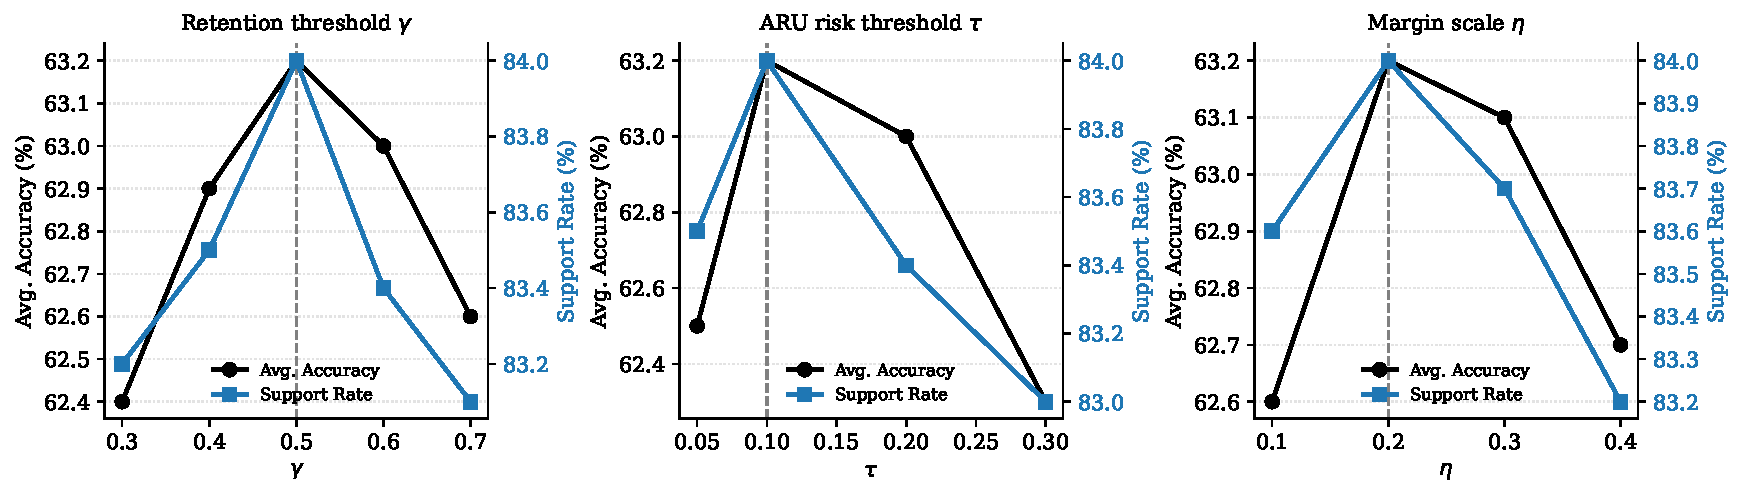
\includegraphics[width=\columnwidth]{sensitivity.pdf}%
    }{%
        \fbox{\parbox[c][0.22\textheight][c]{0.95\columnwidth}{\centering
        Sensitivity figure}}
    }
    \caption[Sensitivity analysis of Fa-DPO.]{Sensitivity analysis of Fa-DPO on the representative II-Medical-8B paired setting. From left to right, we sweep the negative-response retention threshold $\gamma$, the \deleted{ARU-level faithfulness-risk threshold}\added{ARU-level verification-score threshold}\revtag{R1.1} $\tau$, and the sample-level margin scale $\eta$, while fixing all other settings to the defaults in Appendix~\ref{app:training_details}. The black curve (left axis) reports macro-average Accuracy (\%) over MedBullets-op4, MedBullets-op5, MedXpertQA, and MedQA, and the blue curve (right axis) reports Support Rate (\%) on the MedCaseReasoning~\cite{wu2025medcasereasoning} same-answer subset. The vertical dashed lines mark the default values used in the main experiments.}
    \label{fig:sensitivity}
\end{figure}

\subsection{Analysis of Faithfulness Gains}
\label{subsec:faithfulness_gains}

\deleted{We analyze the faithfulness gains of Fa-DPO from two complementary views on the representative II-Medical-8B paired setting.}
\added{This subsection asks where the process gains appear and whether they are visible beyond automatic scores. We first measure ARU-level unfaithfulness by reasoning function to locate the changes inside the reasoning chain. We then use blind pairwise reasoning evaluation on the same-answer setting to test whether the same direction is visible in holistic comparison.}

\subsubsection{ARU-Level Unfaithfulness Shift}
\label{subsec:aru_shift}

We first examine how the observed \deleted{process-faithfulness}\added{automatic process-metric}\revtag{R1.1,R2.1} gains are distributed within the reasoning chain. The II-Medical-8B~\cite{intelligentinternet2025iimedical8b} pair serves as the representative analysis case because it is the strongest paired system in Table~\ref{tab:matched_main_results}, and Appendix~\ref{app:process_metrics} reports the full same-answer process metrics. Here, we focus on the function-wise unfaithfulness shift across ARUs.

\begin{table}[htbp]
    \centering
    \footnotesize
    \caption[ARU-level unfaithfulness shift after Fa-DPO training.]{ARU-level unfaithfulness shift after Fa-DPO training for the II-Medical-8B~\cite{intelligentinternet2025iimedical8b} matched pair on the MedCaseReasoning same-answer hard subset ($n=100$). An ARU is counted as unfaithful when the verifier assigns a neutral or contradiction label to it against its verification premise. Columns report the overall rate (\textit{All}) and the function-wise rates for observation (\textit{O}), warrant (\textit{W}), differentiation (\textit{D}), and claim (\textit{C}) ARUs. The \deleted{Standard DPO and Fa-DPO}\added{Standard DPO-Retained-34K and Fa-DPO-Retained-34K}\revtag{R1.10} rows report pooled unfaithfulness rates for each reasoning function, and the $\Delta$ row reports the absolute percentage-point change. The confidence interval is computed from question-level paired rate differences to avoid treating non-aligned ARUs as independent samples.}
    \label{tab:iimedical_aru_shift}
    \begin{adjustbox}{max width=\columnwidth}
    \begin{tabular}{lccccc}
        \toprule
        \textbf{Metric} & \textbf{All} & \textbf{O} & \textbf{W} & \textbf{D} & \textbf{C} \\
        \midrule
        Std. DPO-Retained-34K (\%) & 22.1 & 12.6 & 32.4 & 36.8 & 29.1 \\
        Fa-DPO-Retained-34K (\%) & 15.4 & 8.9 & 22.8 & 25.9 & 20.7 \\
        $\Delta$ (pp) & -6.7 & -3.7 & -9.6 & -10.9 & -8.4 \\
        95\% CI & [-11.6, -2.7] & [-6.8, -1.1] & [-16.2, -3.8] & [-18.4, -4.1] & [-15.0, -2.1] \\
        \bottomrule
    \end{tabular}
    \end{adjustbox}
\end{table}

\deleted{reasoning--answer}
\deleted{Overall, this function-wise pattern is consistent with the intended effect of Fa-DPO: it reduces unfaithful steps throughout the reasoning process rather than only correcting the final decision.}
\added{Table~\ref{tab:iimedical_aru_shift} localizes the process gain. Overall ARU-level unfaithfulness drops from 22.1\% to 15.4\%, and every ARU type improves with confidence intervals excluding zero. The largest reductions appear in differentiation (-10.9 pp) and warrant ARUs (-9.6 pp), while claim ARUs also decrease by 8.4 pp. The gain is therefore strongest in medically inferential reasoning units, but it remains visible across the full chain.}

\subsubsection{Blind Pairwise Reasoning Evaluation}
\label{subsec:gpt4_eval}

We next test whether the representative same-answer gains remain visible under holistic pairwise judgment. To do so, we use a blind LLM judge \added{as an auxiliary comparative reader}\revtag{R1.15} at fixed answer correctness, since final accuracy alone does not distinguish faithful from unfaithful reasoning.

\paragraph{Experimental Setup.}
\deleted{Standard DPO and Fa-DPO variants}
\deleted{A blind LLM judge}
\deleted{In the reported experiments, we instantiate the blind judge with \texttt{GPT-5.4}.}
\added{We construct a same-answer hard subset of $n=100$ MedCaseReasoning~\cite{wu2025medcasereasoning} chains for the representative II-Medical-8B~\cite{intelligentinternet2025iimedical8b} pair. The compared systems are the II-Medical-8B~\cite{intelligentinternet2025iimedical8b} Standard DPO-Retained-34K and Fa-DPO-Retained-34K variants used in Sec.~\ref{subsec:aru_shift}. Both models predict the correct final diagnosis on these items, while the retained cases still require multi-step reasoning. The test asks whether a blind judge prefers the reasoning produced by Fa-DPO when outcome accuracy is held fixed. A blinded GPT-5.5 LLM judge\footnote{The requested judge model identifier is \texttt{gpt-5.5}, accessed through a proprietary chat API. We report the prompt, decoding settings, requested model identifier, API-returned snapshot logging, and raw-output logging in Appendix~\ref{app:gpt4_protocol}.} performs a pairwise comparison across three dimensions:}
\begin{enumerate}
    \item Hallucination Freedom: Does the chain contain fabricated medical facts?
    \item Logical Coherence: Is the derivation step-by-step sound?
    \item Overall Preference: Which response would a clinician prefer?
\end{enumerate}
\deleted{Appendix~\ref{app:gpt4_protocol} reports the blind-evaluation prompt, order-randomization rule, tie policy, bootstrap confidence-interval protocol, prompt-sensitivity checks, and a separate LLM-judge check. We use GPT-5.5 for this auxiliary role because the task is a blinded, response-level comparative judgment over complete clinical reasoning chains, including coherence and clinically salient support patterns that are difficult to reduce to exact string matches or ARU-level counts. Its proprietary status nevertheless limits strict reproducibility, so this analysis is not used as the primary evidence for the paper's claims. The main evidence comes from matched final-answer accuracy, automatic ARU/NLI-based process metrics backed by parser and routed-NLI validation, and clinician audits; the LLM-judge result is used only to triangulate whether the same direction is visible under holistic pairwise reading.}
\added{Appendix~\ref{app:gpt4_protocol} reports the blind-evaluation prompt, order-randomization rule, tie policy, bootstrap confidence-interval protocol, prompt-sensitivity checks, and a separate LLM-judge check.}
\added{We use GPT-5.5 only as an auxiliary comparative reader for complete clinical reasoning chains. Its proprietary status limits strict reproducibility, so the LLM-judge result is used only to triangulate whether the same direction is visible under holistic pairwise reading; the primary evidence remains matched accuracy, automatic ARU/NLI-based process metrics, parser/verifier validation, and clinician audits.}

\paragraph{Results Analysis.}
\deleted{the faithfulness improvements}
\deleted{Taken together, these blind-judge results show that the representative same-answer gains are not only measurable under verifier-derived metrics but also perceptible under end-to-end comparative evaluation.}
\added{Figure~\ref{fig:win_rate} shows a consistent Fa-DPO preference across all three judged dimensions. The strongest margin is on \textit{Hallucination Freedom} (68/20/12 win/tie/loss), followed by \textit{Overall Preference} (63/22/15); \textit{Logical Coherence} remains positive but has more ties (57/25/18). Prompt-sensitivity checks preserve the same direction, with mean non-tie Fa-DPO win rates of 83.0\%, 74.4\%, and 79.0\% for the three criteria and Fleiss $\kappa=0.63$--0.71. A separate medical-reasoning-rubric call also preserves the direction. Because all checks remain LLM-based, we treat them as supplementary evidence that the same-answer process gains are perceptible under holistic comparison, not as a replacement for clinician audits or ARU-level verifier validation.}

\begin{figure}[htbp]
    \centering
    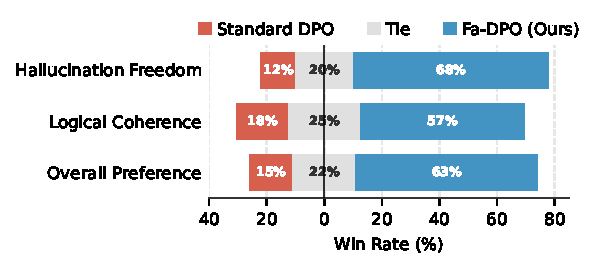
\includegraphics[width=0.6\columnwidth]{win_rate.pdf}
    \caption[Head-to-head comparison on reasoning quality.]{Head-to-head comparison on reasoning quality. Diverging bar chart of blind-judge preferences for the II-Medical-8B~\cite{intelligentinternet2025iimedical8b} matched pair on a MedCaseReasoning~\cite{wu2025medcasereasoning} same-answer subset ($n=100$). The chart is centered at 0\% (Tie). Bars to the right indicate \deleted{Fa-DPO}\added{Fa-DPO-Retained-34K}\revtag{R1.10} wins, and bars to the left indicate \deleted{Standard DPO}\added{Standard DPO-Retained-34K}\revtag{R1.10} wins. The observed win/tie/loss ratios are 68/20/12 for \textit{Hallucination Freedom}, 57/25/18 for \textit{Logical Coherence}, and 63/22/15 for \textit{Overall Preference}.}
    \label{fig:win_rate}
\end{figure}

\deleted{Taken together, these two analyses show that Fa-DPO improves faithfulness both within the reasoning chain and in holistic pairwise judgments at fixed answer correctness.}
\noindent Together, these analyses show where the process gain appears: Fa-DPO reduces unfaithful reasoning units, especially inferential ones, and the same direction is visible in supplementary blind pairwise judgment. We next check the evidence sources and limits behind this interpretation.

\subsection{Evidence Validation and Limits}
\label{subsec:evidence_validation}

\deleted{We next assess whether the evidence used in the preceding analyses is reliable.}
\added{The final experiment block checks the evidence sources behind the preceding claims and states their limits. We organize the checks around clinician and preference-data audits, parser and verifier validation, held-out natural-error analysis, and expert-alignment and clinical-safety diagnostics. Together, these checks support the direction of the Fa-DPO gains while keeping automatic process metrics as diagnostic indicators rather than clinician-adjudicated ground truth.}

\subsubsection{\added{Clinician and Preference-Data Audits}\revtag{R1.9,R1.12,R2.1,R2.5}}
\label{subsec:same_answer_clinician_validation}
\label{subsec:negative_audit}
\label{subsec:preference_label_audit}

\added{The clinician audits provide two checks on the data behind the main mechanism claims. First, the same-answer audit shows that clinicians prefer Fa-DPO's reasoning when final-answer correctness is fixed, matching the direction of the automatic process metrics. Second, the retained-pool audit shows that most sampled constructed negatives remain coherent, clinically plausible, and model-like after risk-based retention, while the strict accept-for-training rate is 65.0\% under all criteria (95\% Wilson CI: 60.2--69.5\%). Agreement on the 100 double-annotated items is strong for target-type match and answer-policy compliance, acceptable for single-error dominance and strict accept-for-training, and moderate-to-good for the ordinal naturalness and plausibility dimensions. The preferred-response and pair-direction audit further shows that the preferred side is reliable but that the pairwise DPO labels are not perfect. We therefore treat the retained dataset as clinically enriched but noisy controlled supervision rather than as fully clinician-ranked RLHF data. Appendix~\ref{app:negative_protocol} reports the detailed negative-audit table, and Appendix~\ref{app:preference_label_details} reports the preferred-response, pair-direction, and w/o-F1 sensitivity details.}\revtag{R1.9,R1.12,R2.1,R2.5,R4.3}

\subsubsection{\added{Parser and Verifier Validation}\revtag{R1.6,R1.16,R2.3,R2.7}}
\label{subsec:aru_parser_validation}
\label{subsec:verifier_validation}

\deleted{The parser and verifier checks test whether the automatic pipeline can support the process-level analyses. The held-out parser validation meets the span and role targets at the primary IoU threshold, but this pass result is not a complete validation of the process evidence. The lower role macro-F1 means that role-specific ARU analyses, especially for minority roles, may contain class-specific misassignment and should not be read as exact prevalence estimates. The low final-answer claim-span F1 means that claim-level consistency can be sensitive to how the normalized answer span is extracted, although benchmark final-answer accuracy is computed independently of the ARU parser. These weaknesses limit the absolute and role-specific interpretation of parser-derived process metrics. They do not directly affect the independently measured answer-accuracy gains, and they do not by themselves establish or refute the reasoning-quality claim. We therefore state the reasoning conclusion as directional automatic process evidence that is supported by clinician audits rather than as clinician-adjudicated absolute faithfulness. The held-out routed NLI verifier reaches 0.838 accuracy, 0.827 macro-F1, expected calibration error 0.064, and Brier score 0.213 on the in-pipeline medical split. The natural-output stress test shows moderate degradation, especially through increased high-risk false negatives, so we keep automatic process metrics as diagnostic indicators. The clinician false-positive audit partly bridges this gap: among verifier-flagged high-risk ARUs, clinicians judge 76.5\% as true errors and only 3.5\% as severe false positives. A separate role- and mask-balanced training-mask audit directly checks strict evidence-support contamination. Among ARUs adjudicated as directly supported or entailed/necessary inferences, the weighted mask-positive rate is 6.9\%, and the severe contradiction-dominant rate is 0.2\%. Clinically acceptable but evidence-unsupported ARUs are reported separately as 76/200 cases (38.0\%), with a weighted mask-positive rate of 34.3\%, and are not counted as gold-entailment false positives. Together with the same-answer clinician audit, these checks form a layered validation package: the same-answer subset isolates process differences under fixed answer correctness, parser validation tests whether ARUs are recoverable, verifier validation bounds the automatic scoring signal and its distribution shift, and clinician audits test whether the diagnostic improvements align with clinical judgments. Appendix~\ref{app:aru_parser_validation} and Appendix~\ref{app:nli_validation} report the detailed protocols and tables.}
\added{The parser and verifier checks characterize whether the automatic pipeline is adequate for bounded process-level proxy analyses. In held-out parser validation, the parser meets the main span and role targets at the primary IoU threshold, but we still treat parser-derived metrics as approximate. Role macro-F1 is lower than the aggregate pass result, so role-specific ARU counts, especially for minority roles, should be read as directional rather than exact. Final-answer claim-span F1 is also low, which means claim-level consistency may depend on answer-span extraction. This limitation does not affect benchmark answer accuracy, which is computed outside the ARU parser.}

\added{The held-out routed NLI verifier reaches 0.838 accuracy, 0.827 macro-F1, expected calibration error 0.064, and Brier score 0.213 on the in-pipeline medical split. The natural-output stress test shows moderate degradation, including a high-risk false-negative increase from 0.118 to 0.172, so we interpret automatic process metrics as diagnostic proxy indicators rather than treating the verifier as a complete checker for natural-output reasoning. The clinician false-positive audit supports this reading: among verifier-flagged high-risk ARUs, clinicians judge 76.5\% as true errors and 3.5\% as severe false positives. In the role- and mask-balanced training-mask audit, directly supported or necessary-inference ARUs have a weighted mask-positive rate of 6.9\% and a severe contradiction-dominant rate of 0.2\%. Clinically acceptable but evidence-unsupported ARUs are reported separately (76/200 cases; 38.0\%) and are not counted as gold-entailment false positives. Overall, these checks support a directional reading of the process metrics, with detailed protocols and tables reported in Appendix~\ref{app:aru_parser_validation} and Appendix~\ref{app:nli_validation}.}

\subsubsection{\added{Held-Out Natural-Error Analysis}\revtag{R1.9,R2.2,R2.6}}
\label{subsec:heldout_natural_error_analysis}

\added{As a task-aligned check, we add a held-out natural-generation analysis for the representative II-Medical-8B matched pair on 3,338 cases from MedXpertQA-test, MedBullets-op4, MedBullets-op5, and MedQA-test. Unlike the controlled counterfactual training negatives, this analysis compares model-sampled Standard DPO-Retained-34K and Fa-DPO-Retained-34K responses on the same held-out prompts without local rewriting.}\revtag{R1.9,R2.2,R2.6}

\added{The annotation source is a frozen official-answer-aware response-level annotation run over these natural model generations: answer correctness is taken from official wrong-case files when available, and each row contains one generated response with the prompt, answer options, gold option, predicted option, and visible reasoning. The label definitions follow the evidence-grounded F1--F4 schema but are applied to natural outputs. F1 marks omission or substantive weakening of clinically important question evidence, F2 marks incorrect medical interpretation of evidence that the response uses, F3 marks overstatement beyond what the available facts support, and F4 marks a selected answer that is unsupported by or inconsistent with the preceding reasoning. An unmapped error is a substantive medical reasoning or knowledge error not cleanly captured by F1--F4; unsupported medical claim and harmful recommendation are recorded as separate safety-relevant flags. To keep the analysis internally consistent, we used conservative decision rules, a fixed JSON schema, one frozen automatic annotation run at temperature 0, post-hoc normalization of allowed labels, and obtained zero judge failures in the reported run. These labels are automatic rather than double-clinician-adjudicated, so they support a fixed-protocol consistency check rather than definitive clinical ground truth. The labels are multi-label: F1--F4 may co-occur with one another and with unmapped, unsupported-claim, or harmful-recommendation flags. Thus, \textit{Any mapped F1--F4} is the response-level OR over F1--F4, and the table rows are not mutually exclusive.}\revtag{R1.9,R1.17,R2.2,R2.6}

\begin{table*}[htbp]
    \centering
    \begingroup\color{blue}
    \footnotesize
    \caption{\added{Held-out task-aligned natural-error analysis on model-sampled responses from the representative II-Medical-8B matched pair. The analysis uses 3,338 held-out cases from MedXpertQA-test, MedBullets-op4, MedBullets-op5, and MedQA-test. Deltas are Fa-DPO-Retained-34K minus Standard DPO-Retained-34K.}\revtag{R1.9,R2.2,R2.6}}
    \label{tab:heldout_natural_error_analysis}
    \begin{adjustbox}{max width=0.95\textwidth}
    \begin{tabular}{lrrrr}
        \toprule
        \textbf{Metric} & \textbf{Std. DPO-Retained-34K} & \textbf{Fa-DPO-Retained-34K} & \textbf{$\Delta$} & \textbf{95\% CI} \\
        \midrule
        Micro accuracy & 47.20 & 48.95 & +1.75 & [+0.60, +2.90] \\
        Any mapped F1--F4 error & 70.00 & 62.40 & -7.60 & [-9.30, -5.80] \\
        F1 evidence omission / weakening & 2.40 & 1.80 & -0.60 & [-1.10, -0.10] \\
        F2 evidence misinterpretation & 10.20 & 8.78 & -1.42 & [-2.50, -0.40] \\
        F3 evidence overinterpretation & 10.50 & 8.45 & -2.05 & [-3.30, -0.80] \\
        F4 reasoning-answer mismatch & 56.50 & 48.08 & -8.42 & [-10.10, -6.80] \\
        Unmapped error & 1.10 & 0.96 & -0.14 & [-0.50, +0.20] \\
        Unsupported medical claim & 5.20 & 3.92 & -1.28 & [-2.10, -0.40] \\
        Harmful recommendation & 0.30 & 0.21 & -0.09 & [-0.30, +0.10] \\
        \bottomrule
    \end{tabular}
    \end{adjustbox}
    \endgroup
\end{table*}

\begin{table*}[htbp]
    \centering
    \begingroup\color{blue}
    \footnotesize
    \caption{\added{Standard-DPO-defined strata in the held-out natural-error analysis. Strata are defined from Standard DPO-Retained-34K outputs before inspecting the paired Fa-DPO-Retained-34K outcome. The mapped stratum has at least one mapped F1--F4 error; the unmapped stratum has an unmapped error and no mapped F1--F4 error. Fa-DPO columns report response-level rates within each Standard-DPO-defined stratum and are not an exhaustive partition because annotation flags are multi-label.}\revtag{R2.2,R2.6}}
    \label{tab:heldout_natural_standard_strata}
    \begin{adjustbox}{max width=0.95\textwidth}
    \begin{tabular}{lrrrrr}
        \toprule
        \textbf{Standard-DPO-defined stratum} & \textbf{$n$} & \textbf{Fa-DPO correct, no mapped} & \textbf{Fa-DPO mapped} & \textbf{Fa-DPO unmapped} & \textbf{Fa-DPO harmful} \\
        \midrule
        Mapped F1--F4 error & 2,337 & 27.4 & 66.8 & 1.0 & 0.2 \\
        Unmapped error without mapped F1--F4 & 37 & 21.6 & 18.9 & 54.1 & 0.0 \\
        Unsupported medical claim & 174 & 18.4 & 70.1 & 1.1 & 0.6 \\
        Harmful recommendation & 10 & 20.0 & 60.0 & 0.0 & 20.0 \\
        \bottomrule
    \end{tabular}
    \end{adjustbox}
    \endgroup
\end{table*}

\deleted{Tables~\ref{tab:heldout_natural_error_analysis} and~\ref{tab:heldout_natural_standard_strata} show a bounded natural-generation transfer pattern. Overall, Fa-DPO increases micro accuracy by 1.75 points and reduces any mapped F1--F4 error by 7.60 points, with the largest mapped reduction on F4 reasoning-answer mismatch. Unsupported medical claims also decrease from 5.20\% to 3.92\%. The Standard-DPO-defined strata localize this effect: among the 2,337 prompts where Standard DPO-Retained-34K has a mapped F1--F4 error, Fa-DPO-Retained-34K is correct without a mapped error in 27.4\%, still has a mapped error in 66.8\%, and has an unmapped error in 1.0\%. Among the 37 Standard-DPO prompts with an unmapped error and no mapped F1--F4 error, Fa-DPO remains unmapped in 54.1\% and is correct without a mapped error in 21.6\%. This small unmapped stratum is boundary evidence rather than a stable estimate of broad natural-error coverage. Because this analysis uses task-aligned MQA prompts and automatic annotation categories tied to evidence-grounded answer and reasoning errors, we use it as task-aligned boundary evidence: it supports transfer to model-sampled MQA outputs while preserving the limitation that F1--F4 is not a complete taxonomy of all naturally occurring medical errors and that the labels are not large-scale clinician-adjudicated ground truth.}
\added{Tables~\ref{tab:heldout_natural_error_analysis} and~\ref{tab:heldout_natural_standard_strata} show bounded transfer to natural model generations. Fa-DPO increases micro accuracy by 1.75 points, reduces any mapped F1--F4 error by 7.60 points, and lowers unsupported medical claims from 5.20\% to 3.92\%. The largest mapped reduction is F4 reasoning-answer mismatch. In the Standard-DPO mapped-error stratum, Fa-DPO is correct without a mapped error in 27.4\% of cases, but still has a mapped error in 66.8\%, so the effect is meaningful but far from complete error removal. The small unmapped stratum remains boundary evidence rather than a stable estimate of broad natural-error coverage. Thus, this analysis supports transfer to task-aligned model-sampled MQA outputs while preserving two limits: F1--F4 is not a complete taxonomy, and the labels are automatic rather than large-scale clinician adjudications.}

\subsubsection{\added{Expert Alignment, Clinical Safety, and Shortcut Diagnostics}\revtag{R2.8,R4.2}}
\label{subsec:human_alignment}
\label{subsec:harm_severity_audit}
\label{subsec:answer_shortcut_diagnostic}

\added{At the chain level, the aggregated Faithfulness Risk Score aligns with expert ratings in the score-stratified sample (Pearson $r=-0.82$, $p<0.001$), supporting its use as a ranking signal within this designed setting. To test the main clinical implication within this setting, we also conduct a blinded retrospective clinician harm-severity audit on 200 matched MedCaseReasoning question IDs from the representative II-Medical-8B pair, yielding 400 anonymized responses. In this audit, an unsupported high-stakes claim is a diagnosis-, triage-, treatment-, monitoring-, contraindication-, or reassurance-relevant assertion that is not supported by the case, retrieved evidence, or preceding reasoning and could plausibly affect clinical management if relied on without clinician oversight. The answer-preservation, answer-changing, counterfactual answer, and token-weight diagnostics are reported in Appendix~\ref{app:answer_shortcut_diagnostics}; they weaken an answer-only shortcut explanation but leave residual shortcut risk possible.}\revtag{R2.8,R4.2}

\begin{table*}[htbp]
    \centering
    \footnotesize
    \caption{\added{Retrospective clinician harm-severity audit on paired Standard DPO-Retained-34K and Fa-DPO-Retained-34K outputs for the representative II-Medical-8B pair. Deltas are Fa-DPO-Retained-34K minus Standard DPO-Retained-34K.}\revtag{R4.2}}
    \label{tab:harm_severity_audit}
    \begin{adjustbox}{max width=0.98\textwidth}
    \begin{tabular}{lcccc}
        \toprule
        \textbf{Outcome} & \textbf{Std. DPO-Retained-34K} & \textbf{Fa-DPO-Retained-34K} & \textbf{$\Delta$} & \textbf{95\% CI / test} \\
        \midrule
        Mean harm severity & 0.74 & 0.61 & -0.13 & [-0.24, -0.02] \\
        Moderate/high harm (\%) & 22.5 & 17.0 & -5.5 & [-10.8, -0.8]; McNemar $p=0.042$ \\
        Unsafe recommendation (\%) & 13.0 & 9.5 & -3.5 & [-7.8, +0.3]; McNemar $p=0.085$ \\
        Unsupported high-stakes claim (\%) & 17.5 & 12.0 & -5.5 & [-10.1, -1.2]; McNemar $p=0.018$ \\
        Contradictory recommendation (\%) & 10.5 & 7.0 & -3.5 & [-7.4, +0.4]; McNemar $p=0.074$ \\
        Clinician oversight warning (\%) & 20.0 & 15.5 & -4.5 & [-9.2, +0.2]; McNemar $p=0.061$ \\
        \bottomrule
    \end{tabular}
    \end{adjustbox}
\end{table*}

\deleted{Overall, the experiments show that Fa-DPO improves faithfulness and answer accuracy under matched comparisons, that these gains can be traced to the intended modules and reasoning-level shifts, and that the supporting evidence further includes held-out ARU parser validation, type-specific clinician validation of the controlled negatives, natural-output verifier shift analysis, harm-severity auditing, answer-changing and counterfactual diagnostics, and score-stratified alignment between faithfulness risk scores and expert ratings.}
\added{Table~\ref{tab:harm_severity_audit} shows modest safety-relevant shifts. Fa-DPO reduces mean harm severity by 0.13, unsupported high-stakes claims by 5.5 points, and moderate/high harm by 5.5 points; unsafe recommendations, contradictory recommendations, and oversight warnings move in the same direction but have intervals that include zero. In non-tie pairwise lower-harm judgments, clinicians prefer Fa-DPO in 62.2\% of cases, but 104 of 200 pairs are ties. The verifier-derived risk score also correlates with clinician-rated harm severity (Spearman $\rho=0.42$, $p<0.001$). These findings support the safety relevance of the process signal, but remain a retrospective audit of one backbone and subset rather than prospective clinical safety validation.}

\added{Taken together, the validation block supports a bounded reading of the experiments. Clinician audits, parser/verifier validation, natural-output diagnostics, and harm-severity auditing all point in the same direction, while also exposing residual failure modes and measurement limits. Overall, the Experiments section supports one central conclusion: Fa-DPO improves matched answer accuracy and automatic reasoning-process metrics, and the gains are tied to the intended construction and optimization design, but the process evidence remains diagnostic and retrospectively validated rather than clinical ground truth.}

\section{Discussion of Results and Implications}
\label{sec:discussion_implications}

\subsection{Discussion of Results}
\deleted{Fa-DPO and Standard DPO}
\deleted{Claim Inconsistency Rate}
\deleted{process-level}
\deleted{Standard DPO}
\added{The results suggest that the main benefit of Fa-DPO comes from improving verifier-derived evidence-use indicators during intermediate clinical reasoning, rather than from only improving final-answer selection. Under same-answer control, Fa-DPO-Retained-34K and Standard DPO-Retained-34K both produce the correct final answer, but Fa-DPO still increases the average Support Rate by 5.1 points and reduces Unsupported Medical Reasoning Rate and Reasoning-Answer Inconsistency Rate by 7.4 and 5.6 points, respectively. This pattern separates automatic process evidence from answer correctness: a model can reach the right answer while still producing reasoning that is verifier-labeled as unsupported, weakly grounded, or internally inconsistent. The matched benchmark results further show that this automatic process-metric improvement is not achieved by sacrificing end-task performance, since Fa-DPO improves macro-average accuracy over Standard DPO-Retained-34K across all six 8B backbones under the same training and evaluation setup.}

\added{Our generalization evidence comes from task-aligned evaluations across multiple evidence-grounded MQA datasets and six diverse 8B backbones, including general-instruction, medical-adapted, and reasoning-enhanced models. These experiments directly match the intended setting of Fa-DPO: improving faithful use of provided clinical evidence in medical question answering. The held-out natural-error analysis further checks model-sampled responses from the representative II-Medical-8B matched pair on 3,338 task-aligned MQA cases and shows that Fa-DPO reduces mapped F1--F4 errors and unsupported medical claims without increasing the small unmapped-error stratum. This supports bounded transfer to natural generations in the same task family for the representative pair, but it does not make F1--F4 a complete taxonomy of all medical hallucination or clinical reasoning errors.}\revtag{R1.17,R2.2,R2.6}

\deleted{In the matched comparisons, the gains cannot be explained by giving the policy model more retrieved evidence at inference time or by filtering outputs after generation; they come from using localized faithfulness risk inside the offline training objective.}
\added{The ablation and mechanism analyses help explain why this improvement occurs. Removing clinically constructed negatives, retrieval-based verification, ARU-level granularity, or either risk-aware objective term consistently weakens performance, which indicates that Fa-DPO works as a coordinated pipeline rather than as a single isolated component. The function-wise ARU analysis and blind pairwise evaluation further show that the gains are visible both in verifier-derived local process indicators and in holistic judgments of reasoning quality. These findings also clarify the empirical distinction between Fa-DPO and prior retrieval, verification, and preference-optimization methods. In the matched comparisons and representative baseline controls, the gains are not explained by positive-only imitation, full-candidate vanilla DPO, sample-count effects, or post-hoc verifier reranking alone. Instead, the strongest single-generation setting uses localized verification scores inside the offline training objective.}

\subsection{Theoretical Implications}
The first theoretical implication is that evidence-grounded MQA should be understood as an evidence-use alignment problem, not only as a retrieval or answer-selection problem. Existing medical RAG systems often emphasize whether relevant evidence can be retrieved and whether the final answer is correct. Our results suggest that these two dimensions are not sufficient. A model may retrieve useful clinical evidence but misinterpret it, overextend it, or fail to connect it to the final answer. Similarly, a correct answer can still be supported by an unfaithful reasoning path. This distinction motivates treating reasoning faithfulness as a separate process-level object of supervision and evaluation.

The second implication is that \deleted{faithfulness measurement}\added{verification}\revtag{R1.1} can be used as an optimization signal rather than only as an evaluation tool. Many verifier-based or self-checking methods detect unsupported claims after generation, during filtering, reranking, or post-hoc correction. Fa-DPO instead converts \deleted{ARU-level faithfulness risk}\added{ARU-level verification scores}\revtag{R1.1} into training-time preference signals. In this sense, the verifier does more than judge whether a response is faithful; it identifies where the reasoning fails and how severe the failure is, allowing the optimization objective to focus more strongly on clinically risky spans.

The third implication concerns preference learning. Standard DPO treats a rejected response mainly as a sequence-level negative example. This is efficient, but it can be coarse for long clinical reasoning chains, where a small number of high-risk claims may be surrounded by otherwise plausible content. Fa-DPO introduces a risk-calibrated view of preference learning: rejected responses are not equally negative, and tokens within a rejected response should not contribute equally when the clinical risk is localized. This view provides a bridge between process-level faithfulness evaluation and offline preference optimization.

\subsection{Practical Implications}
Practically, Fa-DPO provides an offline alignment recipe for evidence-grounded medical QA when online reinforcement learning or dense human reward modeling is costly. Developers can construct faithful-unfaithful preference pairs, verify \added{reasoning-function-labeled ARUs}\revtag{R1.2}\deleted{atomic reasoning units} against routed clinical \deleted{evidence}\added{evidence and reasoning history}\revtag{R1.1}, and use the resulting risk scores to guide preference optimization. This recipe is especially useful when the goal is not only to improve answer accuracy, but also to reduce unsupported intermediate reasoning during model development.

The ARU-level verification pipeline also provides auditable diagnostics for model development. Instead of reporting only whether a model answered correctly, developers can inspect which reasoning units are unsupported, which units contradict retrieved evidence, and which spans carry higher clinical risk. These diagnostics can reveal failure patterns that final-answer accuracy alone cannot show, such as correct answers produced through unstable or weakly supported reasoning.

Finally, the proposed metrics suggest a more informative evaluation protocol for medical QA systems. In addition to final-answer accuracy, system developers should monitor \deleted{Support Rate, Unsupported Medical Reasoning Rate, Contradiction Rate, and Claim Inconsistency Rate}\added{automatic indicators such as Support Rate, Unsupported Medical Reasoning Rate, and Contradiction Rate, and should separately monitor reasoning-answer consistency through Reasoning-Answer Inconsistency Rate}\revtag{R1.1,R2.1}. These \deleted{process-level}\added{diagnostic}\revtag{R1.1,R2.1} indicators can help identify models that appear accurate under multiple-choice evaluation but still produce poorly grounded explanations. At the same time, these implications concern model development and evaluation for evidence-grounded medical QA. They do not replace clinical validation, expert review, or real-world safety assessment before deployment.

\subsection{\added{Computational Cost and Deployment Overhead}\revtag{R4.1}}
\added{The full Fa-DPO pipeline has a one-time offline construction cost before the final model is trained. The raw candidate-generation block starts from 13,092 MedCaseReasoning training positives and four controlled failure types, yielding 52,368 planned rewrite attempts. In our staged implementation, each feasible attempt uses a planning call and a rewrite call, followed by heuristic filtering and judge-model quality control for heuristic-pass candidates; this block yields 47,393 quality-controlled candidates, or 90.5\% of the raw attempts. The archived run did not preserve a complete wall-clock trace for this raw generation and quality-control block, so we report its scale and call structure rather than treating the later verifier timing as an end-to-end construction cost. Overall, the offline construction cost scales with the number of source positives, target failure types, candidate-level LLM calls, ARUs per candidate, routed retrieval queries, and NLI premise pairs; deployment-time inference does not scale with these verifier-side quantities.}\revtag{R4.1}

\added{The measured post-generation construction stages then decompose and score the quality-controlled candidates. In the archived construction run, ARU decomposition, evidence retrieval/reranking, NLI scoring, and preference-file preparation took 47.06 hours in total, dominated by ARU decomposition (39.60 hours), followed by evidence retrieval/reranking (4.32 hours) and NLI scoring (3.07 hours). The retention rule then selected 34,204 retained preference pairs from the quality-controlled pool. These stages produce the retained pairs, risk scores, and token masks before training; they are not executed for each user query.}\revtag{R4.1}

\added{During training, Fa-DPO uses the same 34,204 retained preference pairs as Standard DPO-Retained-34K and adds only precomputed rejected-token weights and a response-level margin to the DPO objective. The archived training logs record 5.19 hours for Standard DPO-Retained-34K and 3.70 hours for Fa-DPO-Retained-34K, but these logs are not a controlled matched training benchmark and should not be used to claim that Fa-DPO is intrinsically faster. They support only the narrower conclusion that the archived run does not show a clear training-time penalty; a fresh matched retraining benchmark would be needed for a precise objective-overhead estimate.}\revtag{R4.1}

\added{At deployment, Fa-DPO is served as a standard single-generation fine-tuned model. We measured Standard DPO-Retained-34K and Fa-DPO-Retained-34K under the same single-GPU serving setting on one NVIDIA A100-SXM4-80GB GPU, using the same MedQA prompts, 5 warmup requests and 100 recorded requests, with maximum output length 512, temperature 0.0, and top-p 0.9. Mean latency was 6.804 seconds for Standard DPO-Retained-34K (SD 0.035; 95\% CI: 6.797--6.812) and 6.808 seconds for Fa-DPO-Retained-34K (SD 0.047; 95\% CI: 6.798--6.817), and the paired mean difference was 0.004 seconds (95\% CI: -0.008--0.014). P95 latency changed from 6.879 to 6.914 seconds. Because the two models share the same architecture after training, this near-identical latency is expected; under this serving setup, the measurement indicates no meaningful deployment-latency penalty for Fa-DPO. Thus, Fa-DPO shifts verifier cost to offline preference construction while keeping inference to one generation without online ARU parsing, evidence retrieval, or NLI scoring.}\revtag{R4.1}

\subsection{\added{Clinical Safety Relevance}\revtag{R4.2}}
\added{Clinical safety is a central motivation for evidence-grounded MQA, but reduced ARU-level violations should be interpreted as a safety-relevant process signal rather than direct evidence of reduced real-world harm or deployment safety. The clinician harm-severity audit in Table~\ref{tab:harm_severity_audit} provides preliminary retrospective support for this link: the observed differences favor Fa-DPO on mean harm severity, moderate/high-harm responses, and non-tie lower-harm pairwise judgments. These effects are modest, and the pairwise audit contains many ties, so the result should be read as a safety-relevant retrospective process signal rather than deployment safety evidence. The findings are consistent with reductions in unsupported and contradictory reasoning, but the audit is retrospective, limited to paired MedCaseReasoning outputs from one representative backbone, and does not replace prospective clinical validation, deployment monitoring, or expert review.}\revtag{R4.2}


\section{Conclusion and Future Work}
This paper presented Fa-DPO, an offline DPO framework for evidence-grounded MQA that injects \deleted{verifier-derived faithfulness risk signals}\added{ARU-level verification scores}\revtag{R1.1} into preference optimization. Across six paired 8B base models, Fa-DPO improves \deleted{verifier-derived process-faithfulness proxies under same-answer evaluation and consistently outperforms Standard DPO in final-answer accuracy under the same training setup}\added{answer accuracy and automatic reasoning-process metrics over Standard DPO-Retained-34K under the same training setup}\revtag{R1.1,R1.10,R2.1}, while remaining competitive with strong released baselines. \deleted{The representative same-answer analyses, blind pairwise evaluation on the II-Medical-8B same-answer hard subset, and score-stratified correlation with expert ratings further suggest that the observed gains are associated with more faithful reasoning rather than answer-only shortcuts.}\added{Control analyses indicate that these gains are better explained by improved reasoning-process behavior than by positive-only SFT, vanilla DPO, sample-count effects, reranking, or answer-only shortcuts.}\revtag{R1.10,R2.4,R2.8}

\deleted{Several limitations remain. The current evidence is restricted to 8B models and multiple-choice MQA, and the pipeline depends on offline negative construction, ARU parsing, retrieval, and NLI verification.}\added{The evaluation remains bounded: experiments use 8B models, evidence-grounded multiple-choice MQA, and controlled negative construction with ARU parsing, retrieval, and NLI verification. Some process metrics are computed using the same ARU/NLI verification framework that provides training signals. Therefore, these metrics should not be interpreted as fully independent proof of faithfulness. We address this limitation by reporting answer accuracy and clinician audits as complementary evidence.}\revtag{R1.9,R1.16,R1.17,R2.1,R2.2,R2.3,R2.6,R2.7} \added{The added audits are mostly retrospective and partly automatic; they do not establish broad hallucination detection or deployment safety, and the retained negatives do not cover the full distribution of naturally generated medical-LLM errors.}\revtag{R1.1,R1.9,R1.12,R1.16,R1.17,R2.2,R2.6,R2.8,R4.2,R4.3} \deleted{Overall, the present results establish a stronger process-faithfulness case for preference optimization in MQA, while future work should extend the evaluation to broader model scales and more open-ended clinical settings, and further strengthen verifier-side and clinician-side validation.}\added{Future work should test Fa-DPO in larger, open-ended clinical settings, combine controlled negatives with model-sampled, clinician-ranked preference data, and strengthen parser, verifier, and clinician validation. Fa-DPO improves answer accuracy and automatic reasoning-process metrics, with clinician audits providing additional support that unsupported and safety-relevant reasoning patterns are reduced.}\revtag{R1.9,R1.12,R2.1,R2.3,R2.7,R4.2}

\appendix

\noindent\textbf{Appendix roadmap.}
\added{Appendix~A documents controlled data construction, including candidate generation, filtering, retained-pool characterization, representative examples, and clinician audit details. Appendix~B reports preference-label reliability and the F1 sensitivity check. Appendix~C gives the verifier-side retrieval and routed-premise protocol. Appendix~D records training settings, faithfulness-oriented baselines, token-weight normalization, component-interaction ablations, and sensitivity analyses. Appendix~E defines the same-answer process-metric protocol and reports full-test, correctness-stratified, and clinician-validation checks. Appendix~F documents ARU parsing and held-out parser validation, while Appendix~K reports NLI verifier validation; Appendices~G--J provide complementary expert-rating, LLM-judge, answer-shortcut, and reverse-entailment diagnostics.}
\section{Controlled Negative Generation Protocol}
\label{app:negative_protocol}

This appendix documents the protocol used to construct the controlled negatives in Sec.~\ref{sec:cot}. The implementation uses \deleted{a named generation script}\added{a staged generation script} and a single generator model $\mathcal{M}$ within each run. The concrete runtime model identifier is configured through the script arguments\footnote{In the reported experiments, we instantiate $\mathcal{M}$ with \texttt{Qwen3-Next-80B-A3B-Instruct}~\cite{yang2025qwen3}.} and is written into the output metadata together with the generation configuration. \added{The protocol constructs controlled counterfactual negatives; it is not a model-sampled human-ranking protocol intended to reproduce the full natural error distribution.}\revtag{R1.9/R4.3}

\subsection{Source Data and Generation Workflow}

We start from the MedCaseReasoning~\cite{wu2025medcasereasoning} training split and, for each positive response, attempt to construct one controlled negative for each target type in $\{F1,F2,F3,F4\}$. \added{The preferred response is the source positive reasoning-answer response from that training example, recorded in our training files as the \texttt{chosen} or correct reasoning-answer field; it is not newly generated by the controlled-rewrite model.}\revtag{R1.12} To keep the notation consistent with the main text, we write a positive response as $y_w = c^{+} \oplus a^{+}$ and a candidate negative response as $\tilde{y}_l = c^{-} \oplus a^{-}$. The implementation follows a staged plan--rewrite pipeline:
\begin{enumerate}[leftmargin=*]
    \item \textbf{Plan stage.} The generator reads the patient context $x$, retrieved evidence $G$, positive reasoning component $c^{+}$, positive final answer $a^{+}$, and the target error type. It returns five fields in JSON: whether a local rewrite is feasible, whether the final answer should be preserved, the target span to edit, a short rationale, and a confidence score.
    \item \textbf{Rewrite stage.} Conditioned on the approved plan, the generator rewrites only the selected local span and returns the negative reasoning, the paired final answer, the modified spans, a short self-check, and an edit summary.
    \item \textbf{Patch materialization.} Under the default span-level patch mode, the edited span is applied back to the original positive reasoning so that the surrounding structure, numbering, and stylistic scaffolding remain unchanged whenever possible.
    \item \textbf{Filtering and review.} The candidate negative response then passes through heuristic filtering and an independent judge-model review stage before entering the quality-controlled candidate pool used for risk measurement.
\end{enumerate}

\subsection{Prompt Structure and Runtime Defaults}

The prompt family contains three templates: a \textit{plan prompt}, a \textit{rewrite prompt}, and a \textit{judge prompt}. The plan prompt asks whether a local controlled edit is feasible and which contiguous span should be changed. The rewrite prompt enforces one dominant target error, preservation of the original topic and style, and answer preservation for F1--F3. In the reported experiments, the judge prompt is enabled as an additional QC stage and independently verifies realized error type, single-error dominance, answer-policy compliance, clinical plausibility, faithfulness drop, and the final accept/review/reject decision.

Table~\ref{tab:negative_protocol_defaults} summarizes the default script configuration used to define the generation protocol.

\begin{table}[htbp]
    \centering
    \caption{Default protocol used by the negative-generation script.}
    \label{tab:negative_protocol_defaults}
    \begin{tabular}{lp{0.60\columnwidth}}
        \toprule
        \textbf{Component} & \textbf{Setting} \\
        \midrule
        Positive source & MedCaseReasoning train split \\
        Error targets & All four controlled types: F1--F4 \\
        Pipeline mode & Staged plan $\rightarrow$ rewrite \\
        Rewrite strategy & Span-level patching of one contiguous local span \\
        Plan decoding & Low-temperature decoding (temperature 0.2; max 220 tokens) \\
        Rewrite decoding & Low-temperature decoding (temperature 0.3; max 900 tokens by default) \\
        Answer policy & F1--F3 preserve the final answer; F4 allows only a small predefined minority of answer changes \\
        Output format & JSON fields for feasibility, target span, rewritten trace, modified spans, self-check, and edit summary \\
        Judge review & Enabled independent review prompt with deterministic decoding (temperature 0) \\
        \bottomrule
    \end{tabular}
\end{table}

\subsection{Automatic Quality Control and Candidate Pool Definition}

After rewrite generation, each raw candidate negative response is screened by a set of heuristic filters before risk measurement and any downstream clinician-audit sampling:
\begin{itemize}[leftmargin=*]
    \item \textbf{Non-trivial local edit:} the rewritten trace must be non-empty and not effectively identical to the positive reasoning.
    \item \textbf{Similarity band:} the sequence similarity between positive and negative reasoning must remain within $[0.55, 0.98]$.
    \item \textbf{Length control:} the token-length ratio between negative and positive reasoning must remain within $[0.6, 1.5]$.
    \item \textbf{Novelty bound:} the ratio of novel tokens introduced by the rewrite must not exceed 0.4.
    \item \textbf{Topic retention:} the rewritten reasoning must maintain at least minimal overlap with the patient context.
    \item \textbf{Answer-policy compliance:} F1--F3 must preserve the final answer exactly, and F4 follows its run-time answer-preservation policy.
    \item \textbf{No meta-language:} candidate negative responses containing dataset-like or self-referential phrases (e.g., ``flawed reasoning'' or ``negative sample'') are removed.
\end{itemize}

In the reported experiments, a second model then reviews every heuristic-pass candidate negative response and receives the patient context $x$, retrieved evidence $G$, positive reasoning component $c^{+}$, positive final answer $a^{+}$, candidate negative reasoning component $c^{-}$, candidate negative final answer $a^{-}$, requested error type, and the plan-stage metadata. It returns a structured JSON record with the realized dominant error type, target-type match, single-error flag, answer-preservation judgment, clinical plausibility score, faithfulness-drop score, off-topic flag, and a final decision in $\{\texttt{accept},\texttt{review},\texttt{reject}\}$.
The initial generation stage attempts 52,368 raw negative candidates from 13,092 source positives and four controlled failure types. Automatic heuristic filtering and judge-model QC accept 47,393 candidates, or 90.5\% of the raw candidates. These accepted candidates form the quality-controlled candidate pool for ARU-level \deleted{faithfulness-risk measurement}\added{verification scoring}\revtag{R1.1}; they are not yet the final DPO preference pairs.

\subsection{Judge-Model QC in the Reported Candidate Pool}

The judge stage is enabled for the reported quality-controlled candidate pool and is executed after heuristic filtering with deterministic decoding. Its role is not to regenerate the sample, but to provide an independent QC decision on whether the candidate negative response remains a usable controlled negative response for later risk measurement. A candidate negative response is accepted into the quality-controlled candidate pool only if the judge decision is \texttt{accept}, the realized dominant error type matches the requested target type, the edit remains single-error rather than mixed, the response is not flagged as off-topic, and answer preservation is confirmed whenever the plan requires it. Candidate negative responses with decision \texttt{review} are written to a separate human-review file and are excluded from the reported candidate pool by default. Candidate negative responses that fail these conditions are written to the rejection file and do not enter later risk measurement or preference alignment. After ARU-level \deleted{faithfulness-risk scoring}\added{verification scoring}\revtag{R1.1}, the retention rule in Sec.~\ref{sec:retention} selects 34,204 candidates as rejected responses, or 72.2\% of the quality-controlled candidates; these retained responses form 34,204 DPO preference pairs.

\subsection{\added{Dataset Bias and Retained-Pool Data Card}\revtag{R4.3}}
\label{app:dataset_bias_details}

\added{Table~\ref{tab:dataset_bias_retention} reports the construction flow and retained-pool diagnostics for the controlled preference dataset. Retention is intentionally risk-enriched rather than prevalence-preserving.}\revtag{R4.3}

\begin{table*}[htbp]
    \centering
    \begingroup\color{blue}
    \footnotesize
    \caption{Type-wise retained-pool composition for the constructed preference dataset.}
    \label{tab:dataset_bias_retention}
    \begin{adjustbox}{max width=\textwidth}
    \begin{tabular}{lrrrrr}
        \toprule
        \textbf{Type} & \textbf{Design-implied raw attempts} & \textbf{Retained pairs} & \textbf{Retained/raw} & \textbf{Share of retained pool} & \textbf{Mean ARUs} \\
        \midrule
        F1 & 13,092 & 6,715 & 51.3\% & 19.6\% & 20.46 \\
        F2 & 13,092 & 9,607 & 73.4\% & 28.1\% & 20.98 \\
        F3 & 13,092 & 9,456 & 72.2\% & 27.6\% & 20.70 \\
        F4 & 13,092 & 8,426 & 64.4\% & 24.6\% & 20.87 \\
        \midrule
        Overall & 52,368 & 34,204 & 65.3\% & 100.0\% & 20.77 \\
        \bottomrule
    \end{tabular}
    \end{adjustbox}
    \endgroup
\end{table*}

\added{Overall, the pipeline generated 52,368 raw rewrite attempts, 47,393 passed automatic QC, and 34,204 were retained after ARU-risk filtering. The overall QC pass rate was 90.5\%, the retained/QC rate was 72.2\%, and the retained/raw rate was 65.3\%.}\revtag{R4.3}

\added{The source-reuse distribution shows that the retained pool repeatedly perturbs many source positives: 62.4\% of source positives contribute three or four retained pairs, accounting for 77.3\% of retained pairs. This improves within-case counterfactual coverage but limits source diversity and may increase overfitting to source cases or case-specific reasoning patterns. The retained-pool composition table further shows that retention is not prevalence-preserving across controlled failure types: F2 and F3 have the highest retained/raw rates and retained-pool shares, F1 has the lowest retained/raw rate and retained-pool share, and F4 remains intermediate. Because type-wise QC/discarded counts are not part of the recorded type-wise construction outputs, we report QC flow only at the overall level and do not attribute type-wise retained/raw differences to a specific QC stage. The retained-pool clinician audit in Table~\ref{tab:negative_quality} shows that the constructed negatives are usually acceptable as controlled counterfactuals after retention. We therefore use the retained pool as controlled, risk-enriched supervision and avoid treating it as a natural-prevalence sample.}\revtag{R4.3}

\begin{table*}[htbp]
    \centering
    \begingroup\color{blue}
    \footnotesize
    \caption{Main dataset-bias sources and how they are handled in the revised manuscript.}
    \label{tab:dataset_bias_sources}
    \begin{adjustbox}{max width=\textwidth}
    \begin{tabular}{p{0.18\textwidth}p{0.39\textwidth}p{0.34\textwidth}}
        \toprule
        \textbf{Bias source} & \textbf{Observed boundary} & \textbf{Manuscript handling} \\
        \midrule
        Source dataset & All preference pairs come from MedCaseReasoning training positives, so source specialty and case-style coverage may not match broader clinical QA; \added{repeated perturbations of the same source cases may also reduce source diversity}\revtag{R4.3}. & We report the source size \added{and source-reuse distribution}\revtag{R4.3} and avoid population-prevalence claims. \\
        Taxonomy & F1--F4 cover evidence-use and reasoning-answer consistency failures in evidence-grounded MQA, not all medical hallucination phenomena. & We restrict external evaluation to task-aligned MQA benchmarks, add a representative held-out natural-error analysis within that task family, and avoid treating hallucination-oriented benchmarks as evidence-use taxonomy tests. \\
        Construction & Local rewrites provide target-type control, and the retained-pool audit shows 65.0\% strict accept-for-training, but constructed responses remain noisy controlled counterfactuals rather than natural model-sampled errors. & We report clinician/audit results, interpret constructed negatives as controlled counterfactuals, and avoid natural-prevalence claims. \\
        Answer policy & F1--F3 preserve the extracted final answer in all retained pairs; F4 preserves it in 84.1\%. & We report answer-preservation and answer-changing diagnostics rather than treating the pool as answer-randomized. \\
        Risk filtering & ARU-risk retention enriches high-risk local failures rather than sampling candidates uniformly \added{and is not prevalence-preserving across failure types}\revtag{R4.3}. & Standard DPO-Retained-34K and Fa-DPO-Retained-34K use the same retained content, isolating the objective effect. \\
        Verifier-induced labels & Parser and NLI outputs determine retention, token masks, and process metrics. & Parser, NLI, and high-risk ARU audits delimit automatic-measurement noise. \\
        Preference labels & Preferred responses are reliable in the audit, but pair direction remains imperfect. & We report preferred-response reliability, pair-direction validity, and w/o-F1 sensitivity. \\
        \bottomrule
    \end{tabular}
    \end{adjustbox}
    \endgroup
\end{table*}

\subsection{Representative Controlled Error Examples}
\label{app:negative_examples}

Table~\ref{tab:negative_examples} provides schematic local edits illustrating the intended perturbation pattern for each controlled error type. These examples are representative templates rather than verbatim released training instances.

\begin{table*}[htbp]
    \centering
    \caption{Schematic local edits for the four controlled process-level failure types.}
    \label{tab:negative_examples}
    \begin{tabular}{p{0.10\textwidth}p{0.28\textwidth}p{0.28\textwidth}p{0.24\textwidth}}
        \toprule
        \textbf{Type} & \textbf{Positive local span} & \textbf{Negative local span} & \textbf{Intended failure} \\
        \midrule
        F1 & ``The normal ejection fraction weakens acute heart failure despite the edema.'' & ``Edema is consistent with acute heart failure,'' with the normal ejection fraction no longer used substantively. & Omit or down-weight key available evidence while preserving the overall case topic. \\
        F2 & ``A BNP of 90 pg/mL offers only weak support for acute heart failure.'' & ``A BNP of 90 pg/mL definitively confirms acute heart failure.'' & Keep the cited evidence but misread its medical meaning. \\
        F3 & ``Edema and mild dyspnea are suggestive but not decisive for cardiogenic pulmonary edema.'' & ``Edema and mild dyspnea definitively establish cardiogenic pulmonary edema.'' & Convert limited support into unjustified certainty or add unsupported evidential strength. \\
        F4 & ``The findings argue against acute decompensated heart failure and favor a non-cardiogenic cause.'' & Reasoning remains as above, but the final answer is still ``acute decompensated heart failure.'' & Break the derivational link between the reasoning and the final answer. \\
        \bottomrule
\end{tabular}
\end{table*}

\subsection{\added{Clinician Audit of Constructed Negative Responses}\revtag{R1.9,R4.3}}
\label{app:negative_audit_details}

\added{The post-retention clinician audit checks whether sampled retained negatives instantiate the intended controlled failure while preserving contextual coherence, clinical plausibility, model-likeliness/naturalness of the injected error, and the required answer policy. The audit uses 400 sampled responses, corresponding to approximately 1.2\% of the retained pool, with 100 items per error type. Five board-certified physicians in internal medicine and emergency medicine serve as reviewers, and 100 items receive double annotation.}\revtag{R1.9,R4.3}

\begin{table*}[htbp]
    \centering
    \begingroup\color{blue}
    \footnotesize
    \caption{Expanded clinician audit of the risk-retained DPO negative pool. All rates are computed on 400 audited retained negatives, stratified as 100 items per F1--F4 type. ``Strict accept'' requires target-type match, single-error dominance, answer-policy compliance, and pass-level contextual coherence, model-likeliness/naturalness, and clinical plausibility. Ordinal pass rates use a threshold of at least 4 on the 1--5 scales.}
    \label{tab:negative_quality}
    \begin{adjustbox}{max width=\textwidth}
    \begin{tabular}{lcccccccccc}
        \toprule
        \textbf{Type} & \textbf{$n$} & \textbf{Type Match} & \textbf{Single Error} & \textbf{Policy} & \textbf{Coherence} & \textbf{Model-like} & \textbf{Plaus.} & \textbf{Faith. Degr.} & \textbf{Strict Accept} & \textbf{Strict 95\% CI} \\
        \midrule
        F1 & 100 & 74.0 & 68.0 & 98.0 & 84.0 & 76.0 & 82.0 & 72.0 & 56.0 & [46.2, 65.3] \\
        F2 & 100 & 84.0 & 78.0 & 99.0 & 91.0 & 86.0 & 89.0 & 80.0 & 70.0 & [60.4, 78.1] \\
        F3 & 100 & 86.0 & 80.0 & 98.0 & 90.0 & 85.0 & 88.0 & 84.0 & 72.0 & [62.5, 79.9] \\
        F4 & 100 & 76.0 & 70.0 & 89.0 & 87.0 & 81.0 & 85.0 & 76.0 & 62.0 & [52.2, 70.9] \\
        \midrule
        Overall & 400 & 80.0 & 74.0 & 96.0 & 88.0 & 82.0 & 86.0 & 78.0 & 65.0 & [60.2, 69.5] \\
        \bottomrule
    \end{tabular}
    \end{adjustbox}
    \endgroup
\end{table*}

\added{Overall, 88.0\% of the assessed constructed negatives pass contextual coherence, 86.0\% pass clinical plausibility, 82.0\% pass the stricter model-likeliness/naturalness criterion, and 78.0\% show pass-level faithfulness degradation, while 65.0\% are accepted as controlled counterfactual negatives under all strict criteria (95\% Wilson CI: 60.2--69.5\%).}\revtag{R1.9,R4.3}

\added{The type-wise results show useful but uneven quality across failure types. Strict accept rates range from 56.0\% for F1 to 72.0\% for F3. F2 and F3 are the most stable categories, whereas the weakest cells are F1 target-type match (74.0\%) and single-error dominance (68.0\%), and F4 answer-policy compliance (89.0\%). This pattern suggests that omission/down-weighting edits are harder to keep as a single dominant controlled error, while reasoning-answer inconsistency edits more often stress final-answer policy constraints.}\revtag{R1.9,R4.3}

\added{The audit is a post-retention clinician check rather than the sole rule used to admit training pairs: before this audit, candidates had already passed heuristic filtering, judge-model QC, and ARU-score-based retention, and the clinician audit was not fed back into the training set. Because Standard DPO-Retained-34K and Fa-DPO-Retained-34K train on the same retained pool, the matched comparison asks whether the Fa-DPO objective extracts a stronger signal from the same controlled data rather than assuming that every retained pair is a perfect clinician-ranked RLHF pair. We therefore interpret the retained negatives as usable but noisy controlled counterfactuals for the target process failures, while still not claiming that local rewriting reproduces the full natural model-error distribution.}\revtag{R1.9,R4.3}

\subsection{\added{Inter-Rater Agreement for the Local Rewrite Naturalness Audit}\revtag{R1.9}}
\label{app:ordinal_agreement}

\deleted{The clinician audit includes three binary judgments---target-type match, single-error dominance, and answer-policy compliance---and two 1--5 ordinal judgments---clinical plausibility and faithfulness degradation.}\added{The expanded local rewrite naturalness audit includes binary judgments for target-type match, single-error dominance, answer-policy compliance, and strict accept-for-training, as well as 1--5 ordinal judgments for contextual coherence, model-likeliness/naturalness, clinical plausibility, and faithfulness degradation.}\revtag{R1.9} Table~\ref{tab:negative_quality} reports the \added{adjudicated}\revtag{R1.9} audit outcomes, while this appendix reports \deleted{agreement on the two ordinal judgments using weighted Cohen's kappa, together with exact and within-1 agreement on}\added{inter-rater agreement on}\revtag{R1.9} the 100 doubly annotated items. \added{The naturalness and coherence judgments are subjective, so we report Cohen's $\kappa$ for binary judgments and quadratic-weighted Cohen's $\kappa$, exact agreement, and within-1 agreement for ordinal judgments.}\revtag{R1.9}

\begin{table}[htbp]
    \centering
    \caption{\added{Inter-rater agreement for the expanded local rewrite naturalness audit, computed on the 100 doubly annotated items.}\revtag{R1.9}}
    \label{tab:ordinal_agreement}
    \begin{tabular}{lccc}
        \toprule
        \textbf{Judgment} & \textbf{$\kappa$} & \textbf{Exact (\%)} & \textbf{Within-1 (\%)} \\
        \midrule
        Target-type match & 0.82 & 91.0 & -- \\
        Single-error dominance & 0.70 & 85.0 & -- \\
        Answer-policy compliance & 0.90 & 96.0 & -- \\
        Strict accept-for-training & 0.72 & 88.0 & -- \\
        Contextual coherence & 0.74 & 76.0 & 97.0 \\
        Model-likeliness/naturalness & 0.76 & 78.0 & 96.0 \\
        Clinical plausibility & 0.68 & 75.0 & 95.0 \\
        Faithfulness degradation & 0.80 & 78.0 & 94.0 \\
        \bottomrule
\end{tabular}
\end{table}

\added{These agreement results support the audit's role as a reliability check, while also showing where the judgments remain subjective. The more rule-like dimensions are stable: target-type match reaches $\kappa=0.82$, answer-policy compliance reaches $\kappa=0.90$, and the derived strict accept-for-training decision reaches $\kappa=0.72$ with 88.0\% exact agreement. The lower bound is clinical plausibility (weighted $\kappa=0.68$), reflecting the expected subjectivity of judging whether a locally injected error remains clinically plausible. However, its within-1 agreement is 95.0\%, and the other ordinal dimensions reach weighted $\kappa=0.74$--0.80 with 94.0--97.0\% within-1 agreement. We therefore base the interpretation on adjudicated labels, confidence intervals, and type-wise results, and describe the retained pool as noisy controlled supervision rather than uniformly clean data.}\revtag{R1.9,R4.3}

\section{\added{Preference-Label Reliability and F1 Sensitivity Details}\revtag{R1.12,R1.15,R1.17}}
\label{app:preference_label_details}

\added{The negative-response audit does not by itself validate the DPO labels, because DPO also assumes that the preferred response $y_w$ is a reliable alignment target and that the pairwise direction $y_w \succ y_l$ is clinically meaningful. The preferred responses audited here are the same MedCaseReasoning source positive responses paired with retained rejected responses, not outputs newly generated by the controlled-rewrite model. We therefore conduct two additional blinded clinician audits on retained training items: a 200-item preferred-response audit and a 200-item pair-level audit, each balanced across the paired F1--F4 rejected-response types with 50 items per type.}\revtag{R1.12,R1.15,R1.17}

\begin{table*}[htbp]
    \centering
    \begingroup\color{blue}
    \footnotesize
    \caption{Clinician audit of preferred-response reliability and pairwise preference-label validity on retained DPO training items. The two samples are balanced across F1--F4 rejected-response types and are intended as targeted label-reliability audits rather than exhaustive quality control over all 34,204 retained pairs.\revtag{R1.12,R1.15,R1.17}}
    \label{tab:preference_label_audit}
    \begin{adjustbox}{max width=0.98\textwidth}
    \begin{tabular}{lccccc}
        \toprule
        \textbf{Audit target} & \textbf{$n$} & \textbf{Primary validity rate} & \textbf{95\% CI} & \textbf{Secondary findings} & \textbf{Agreement} \\
        \midrule
        Preferred responses & 200 & Reliable target: 98.5\% & [95.7, 99.5]\% & Major issue: 1.5\%; final answer correct: 98.5\%; contradiction: 0.0\% & Exact 82.0\%; $\kappa=-0.018$ \\
        Preference pairs & 200 & Direction valid: 76.0\% & [69.6, 81.4]\% & DPO-suitable: 86.0\%; direct reversal: 10.0\%; tie: 14.0\% & Exact 79.0\%; $\kappa=0.662$ \\
        \bottomrule
    \end{tabular}
    \end{adjustbox}
    \endgroup
\end{table*}

\added{The preferred-response side is reliable in this stratified audit: 197/200 preferred responses are judged acceptable or minor-issue-but-usable, with a 1.5\% major-issue rate and no adjudicated contradictions. The negative $\kappa$ for this row should be read in the context of extreme prevalence imbalance: major preferred-response issues are rare after adjudication, so chance-corrected agreement is unstable for this rare-error judgment. We therefore treat the adjudicated reliable-target rate of 98.5\% as the primary evidence for preferred-response quality, rather than treating $\kappa$ as the primary quality measure for this imbalanced binary audit. Pair-level labels are noisier. Clinicians validate the constructed direction in 152/200 pairs and judge 172/200 pairs suitable for DPO training, but 20/200 pairs are direct reversals and 28/200 are ties with no clear preference. The two rates answer different questions: direction validity asks whether the constructed label $y_w \succ y_l$ is clinically correct, whereas DPO suitability asks whether the two responses contain a usable preference contrast after clinician review. Thus, a direct reversal may still reveal a clear contrast but is label noise for the submitted constructed direction; ties are the least suitable for pairwise DPO because no clear preference exists. Among non-tie cases, the constructed direction agrees with the adjudicated clinician direction in 88.4\% of cases. Taken together, these results support the preferred side as a usable target while showing that the retained pairs remain noisy controlled supervision, not clinician-ranked gold-standard RLHF preferences. The audit also exposes a substantive limitation for DPO training: direct reversals can push the pairwise objective in the wrong direction, and ties provide weak or no pairwise preference signal. Because reversal and tie cases are not confined to F1, the F1-exclusion analysis below should be read as a lowest-confidence-type sensitivity check, not as a complete label-denoising experiment.}\revtag{R1.12,R1.15,R1.17}

\begin{table*}[htbp]
    \centering
    \begingroup\color{blue}
    \footnotesize
    \caption{Sensitivity analysis excluding the lower-confidence F1 preference category. Process metrics are \deleted{verifier-derived}\added{automatic ARU/NLI-based}\revtag{R2.1} percentages on the MedCaseReasoning same-answer hard subset, and Avg. Acc. is the macro-average over MedBullets-op4, MedBullets-op5, MedXpertQA, and MedQA.\revtag{R1.12,R1.15,R1.17}}
    \label{tab:f1_exclusion_sensitivity}
    \begin{tabular}{lccccc}
        \toprule
        \textbf{Method} & \textbf{Support $\uparrow$} & \textbf{Contradiction $\downarrow$} & \textbf{Unsupported $\downarrow$} & \textbf{\deleted{Claim Inconsistency}\added{Reason.-Ans. Inconsistency}\revtag{R1.1} $\downarrow$} & \textbf{Avg. Acc. $\uparrow$} \\
        \midrule
        Standard DPO-Retained-34K & 77.3 & 9.4 & 31.6 & 26.1 & 62.0 \\
        Fa-DPO-Retained-34K & \textbf{84.0} & \textbf{5.2} & \textbf{20.9} & \textbf{18.5} & \textbf{63.2} \\
        Fa-DPO-w/o-F1 & 83.2 & 5.5 & 21.8 & 19.2 & 63.0 \\
        \bottomrule
    \end{tabular}
    \endgroup
\end{table*}

\added{Removing F1 slightly weakens the full Fa-DPO result, but the main conclusion remains intact. Compared with Standard DPO-Retained-34K, Fa-DPO-w/o-F1 still improves Support Rate by 5.9 points, reduces Contradiction Rate by 3.9 points, reduces Unsupported Medical Reasoning Rate by 9.8 points, reduces Reasoning-Answer Inconsistency Rate by 6.9 points, and improves average accuracy by 1.0 point.}\revtag{R1.1,R1.12,R1.15,R1.17} \added{We selected F1 for this exclusion sensitivity because it has the lowest type-wise pair-direction validity in the preference-label audit and the lowest strict accept rate in the local-rewrite naturalness audit. F4 is not the lowest category by pair-label validity or by retained-pool naturalness acceptance, and it directly defines the reasoning-answer consistency target; excluding it would answer a target-coverage ablation question rather than a naturalness-validation question. This sensitivity should therefore not be interpreted as removing all pair-level reversal or tie noise from the retained training set. A stronger label-noise test would require a clinician-denoised retained pool in which confirmed reversals are corrected and ties are removed before retraining. This remains a residual limitation: future work should add clinician-ranked natural reasoning-answer inconsistency pairs and denoised preference-pair training.}\revtag{R1.9,R1.12}

\section{Retrieval and Routed-Premise Protocol}
\label{app:retrieval_protocol}

This appendix documents the verifier-side retrieval and verification-premise construction pipeline used in Sec.~\ref{sec:verification}. The policy model does not receive retrieved passages during benchmark inference; retrieval is used only offline for \deleted{faithfulness measurement}\added{verification scoring}\revtag{R1.1} and the dedicated \deleted{process-faithfulness}\added{process-metric}\revtag{R1.1} analyses. \added{This design keeps Fa-DPO and the Standard DPO-Retained-34K baseline under the same policy-input condition; retrieval is reserved for offline construction, verification, and analysis.}\revtag{R3.6}

\subsection{Corpus, Indexing, and Sharing Policy}

We build one fixed verifier-side corpus and keep it unchanged across the matched backbone comparisons, all ablations, and the appendix analyses. This design prevents Fa-DPO from benefiting from a stronger verification-premise budget than the paired \deleted{Standard DPO comparisons}\added{Standard DPO-Retained-34K comparisons}\revtag{R1.10} run under the same settings. The reported protocol therefore summarizes the corpus source and scale, the concrete retriever and reranker identifiers, the route-wise query budgets, and the verification-premise construction rules.

\begin{table}[htbp]
    \centering
    \caption{Verifier-side retrieval and verification-premise pipeline summary. Panel A records the fixed corpus, indexing setup, and retriever configuration. Panel B summarizes the route-wise query formation, retrieval budget, and premise-construction rules.}
    \label{tab:retrieval_protocol_template}
    {\footnotesize
    \setlength{\tabcolsep}{4pt}
    \renewcommand{\arraystretch}{1.12}
    \begin{tabular}{>{\raggedright\arraybackslash}p{0.27\columnwidth}>{\raggedright\arraybackslash}p{0.67\columnwidth}}
        \toprule
        \multicolumn{2}{l}{\textbf{Panel A: Corpus and retriever setup}} \\
        \midrule
        Corpus source & Fixed verifier-side corpus exported from Hugging Face \texttt{miriad/miriad-5.8M}; each record is one title--passage row with metadata such as specialty, year, and paper URL. \\
        \midrule
        Corpus scale & 812,383 distinct papers (unique \texttt{paper\_url}) and 5,821,945 indexed passages; average chunk length 4,667.79 characters or 713.48 whitespace tokens. \\
        \midrule
        Chunking & One \texttt{passage\_text} is one retrieval unit, serialized as \texttt{title [SEP] passage} when a title is available; no sliding-window overlap; passages shorter than 20 characters are dropped. \\
        \midrule
        Sparse branch & \texttt{none}. \\
        \midrule
        Dense branch & \texttt{ncbi/MedCPT-Query-Encoder} over a FAISS \texttt{IndexFlatIP} index built from \texttt{ncbi/MedCPT-Article-Encoder} document embeddings~\cite{jin2023medcpt}. \\
        \midrule
        Fusion / reranking & Dense-only retrieval with no BM25 branch or sparse--dense fusion; rerank retained candidates with \texttt{ncbi/MedCPT-Cross-Encoder}. \\
        \midrule
        Candidate ordering & For multi-query routes, keep within-query retriever rank, merge duplicate texts, sort by best retriever score, best retriever rank, and matched-query count, rerank with the cross-encoder, then retain evidence in descending reranker score with a final deduplication pass. \\
        \bottomrule
    \end{tabular}

    \vspace{0.45em}

    \begin{tabular}{>{\centering\arraybackslash}p{0.10\columnwidth}>{\raggedright\arraybackslash}p{0.33\columnwidth}>{\raggedright\arraybackslash}p{0.47\columnwidth}}
        \toprule
        \multicolumn{3}{l}{\textbf{Panel B: Route-wise premise policy}} \\
        \midrule
        \textbf{Route} & \textbf{Query / retrieval} & \textbf{Premise / decision rule} \\
        \midrule
        $O$ & No external retrieval; score directly against patient-context sentences. If the best context-side check is neutral-dominant, run one auxiliary plausibility check against the row-level retained evidence block without launching a new query. & Patient-context sentences are the primary premise; auxiliary evidence is used only for fallback plausibility checking and does not remove the missing-record penalty. \\
        \midrule
        $W$ & Use the decontextualized \texttt{retrieval\_query} when available; otherwise build heuristic variants from the ARU text. Up to 4 variants per ARU; each retrieves top 50 dense hits, reranks top 50, merges up to 80 unique candidates, and keeps the top 5 texts. & Concatenate the retained evidence texts into one evidence-only premise. \\
        \midrule
        $D$ & Use the same query construction and retrieval budget as $W$; keep the retained texts as the differentiation evidence block $G_i$. & Concatenate the patient context $x$ and retained evidence block $G_i$ into the combined differentiation premise $E_i^{D} = \mathrm{concat}(x, G_i)$. \\
        \midrule
        $C$ & No external retrieval. & Use the serialized reasoning history $H_{i-1} = \mathrm{concat}(v_1, \dots, v_{i-1})$ as the verification premise. \\
        \bottomrule
    \end{tabular}}
\end{table}

Unless otherwise stated, the same verifier-side corpus, index, query encoder, reranker, and retrieval budget are reused across the matched same-backbone comparisons, ablations, and appendix analyses. \deleted{The anonymous artifact records the pipeline scripts, model identifiers, and configuration, while}\added{The appendix records the corpus source, model identifiers, and route-wise configuration, while}\revtag{R1.6} corpus reconstruction follows the upstream \texttt{miriad/miriad-5.8M}~\cite{zheng2025miriad} access terms.

\subsection{Route-Wise Verification Premise Construction}

After the parser produces an ordered ARU sequence, each ARU is assigned a reasoning-function-specific verification premise. To make this construction reproducible, we record for every route the query source, retrieval depth, reranking rule, snippet ordering, and final premise template passed to the verifier.

\begin{itemize}[leftmargin=*]
    \item \textbf{Observation route ($O$).} The primary verification premise is always the patient context $x$, with no external retrieval query. If the best context-side check is neutral/unsupported, we run only an auxiliary plausibility check against the row-level retained evidence block; this auxiliary check does not remove the missing-record penalty.
    \item \textbf{Warrant route ($W$).} The query is the warrant ARU text $v_i$ or its preferred heuristic variant. We retrieve and rerank evidence from the fixed medical corpus, keep the retained texts in descending reranker order, and concatenate them to form the warrant-side evidence premise $G_i$.
    \item \textbf{Differentiation route ($D$).} The query is the differentiation ARU text $v_i$ or its preferred heuristic variant, because these ARUs encode the exclusion criterion and the candidate alternative being ruled out. We retrieve and rerank evidence from the fixed medical corpus, keep the retained texts as $G_i$, and concatenate them with the patient context to form the combined differentiation premise $E_i^{D} = \mathrm{concat}(x, G_i)$.
    \item \textbf{Claim route ($C$).} Claim ARUs do not invoke external retrieval. Their verification premise is the serialized local reasoning history $H_{i-1} = \mathrm{concat}(v_1, \dots, v_{i-1})$, preserving the original ARU order. The final-answer claim ARU uses the same route, so \deleted{answer-faithfulness}\added{reasoning-answer consistency}\revtag{R1.1} is evaluated against the preceding reasoning history rather than against retrieved passages.
\end{itemize}

\deleted{Detailed route-wise retrieval-quality summary metrics are deferred to the supplementary appendix file.}\revtag{R1.6}

\section{Training Hyperparameters and Run Protocol}
\label{app:training_details}

This appendix records the training-side settings \deleted{deferred from}\added{from}\revtag{R1.6} the main-text Implementation Details. Unless otherwise noted, all matched \deleted{Standard DPO and Fa-DPO}\added{Standard DPO-Retained-34K and Fa-DPO-Retained-34K}\revtag{R1.10} runs share the same hardware budget, optimization schedule, and sequence-length limits.

\subsection{Shared Training Configuration}

Each run uses 8 NVIDIA A100 GPUs, learning rate $5\times10^{-7}$, cosine decay, warmup ratio 0.1, one training epoch, and $\beta=0.3$. In the reported 8-GPU launch, the effective batch size is 32 preference pairs, implemented as per-device batch size 1 with gradient accumulation 4 under bf16 mixed precision. We use LoRA~\cite{hu2022lora} with rank 64, LoRA alpha 128, dropout 0.05, and no bias adaptation. The maximum sequence length is 4096 and the maximum prompt length is 2048. The training entry point uses FlashAttention-2 and gradient checkpointing with \texttt{use\_reentrant=False}, logs every 5 steps, and evaluates and saves every 20 steps.

\subsection{\added{Faithfulness-Oriented Baseline Control Protocol}\revtag{R2.4}}
\label{app:faithfulness_baseline_protocol}

\added{The representative baseline controls in Table~\ref{tab:faithfulness_baseline_results} use the II-Medical-8B~\cite{intelligentinternet2025iimedical8b} backbone and the same benchmark splits, prompts, answer-extraction rule, and process-metric pipeline as the matched II-Medical-8B comparison. SFT-faithful trains on the exact preferred-response side ($y_w$) used in the retained preference pairs, deduplicated by prompt and target response; it uses the same tokenizer, optimizer family, LoRA setup, sequence limits, and one-epoch supervised schedule, but it is not an update-matched DPO run because it is a positive-only supervised control. Standard DPO-QC-All uses all 47,393 quality-controlled candidate pairs, Standard DPO-Random-34K uses a random 34,204-pair subset of that QC pool, and Standard DPO-Retained-34K uses the 34,204 ARU-risk-retained pairs. Fa-DPO-Retained-34K uses the same retained pairs as Standard DPO-Retained-34K and adds only the token-level risk weighting and response-level margin. These controls are intended as representative attribution checks, not an exhaustive baseline suite.}\revtag{R1.10,R2.4}

\added{Verifier reranking does not add a new training run. It uses the Standard DPO-Retained-34K generator, samples $K$ responses per question under the same decoding profile, decomposes each candidate into ARUs, scores candidates with the same routed-premise NLI verifier, and selects the response with the lowest response-level risk score. We report both $K=4$ and $K=8$ because larger candidate pools can narrow the performance gap, but Table~\ref{tab:faithfulness_baseline_results} reports only generation count and deployment-time verifier use together with accuracy and process metrics; it does not claim measured reranking latency for either $K$.}\revtag{R2.4,R4.1}

\subsection{Fa-DPO Coefficients and Evaluation Rule}

\paragraph{Retention.}
Fa-DPO retains a constructed negative response when its response-level risk score satisfies $\gamma=0.5$.
\added{This threshold is fixed before the final clinician audit; the audit validates the retained pool rather than tuning $\gamma$.}\revtag{R1.7}
If no paired candidate for a covered source positive passes this threshold, we keep the paired candidate with the largest risk score.
This rule keeps clearly risky negatives while filtering out mildly flawed ones.
It yields 34,204 rejected responses from 12,411 source positives, corresponding to 72.2\% of the quality-controlled candidates.
These retained responses form the 34,204 DPO preference pairs used by both \deleted{Standard DPO and Fa-DPO}\added{Standard DPO-Retained-34K and Fa-DPO-Retained-34K}\revtag{R1.10} in the matched comparisons.

\paragraph{Token weighting and response severity.}
The token reweighting mask in Eq.~\ref{eq:topology_mask} uses $\alpha=2.0$, $\epsilon=0.1$, and ARU-level \deleted{faithfulness-risk}\added{verification-score}\revtag{R1.1} threshold $\tau=0.1$ inside the weighted rejected log-ratio in Eq.~\ref{eq:weighted_rejected_logratio}. \added{With these default values and $s_i\in[0,1]$, the raw mask satisfies $m_t\in[0.1,3.0]$, so the normalized effective token weight is bounded above by $(1+\alpha)/\epsilon=30$, while $\sum_t\omega_t=T_l$ keeps the rejected-side total token mass fixed for each rejected response.}\revtag{R1.4}
The raw severity score in Eq.~\ref{eq:severity_raw} uses $\omega_{\text{peak}}=0.6$, $\omega_{\text{cov}}=0.4$, and $\omega_{\text{mean}}=0.1$.
These weights place the largest emphasis on the worst local failure, a secondary emphasis on how broadly high-risk ARUs appear, and a smaller stabilizing emphasis on overall defect density.
Because each component lies in $[0,1]$, this setting gives $S_{\text{raw}}(y_l)\in[0,1.1]$.
Eq.~\ref{eq:faithfulness_risk_score} then normalizes the response-level risk score to $[0,1]$.

\paragraph{Risk-adaptive margin.}
The margin mapping in Eq.~\ref{eq:severity_margin} uses $\eta=0.2$, $\kappa_{\delta}=3.0$, and $c_{\text{sat}}=2.5$.
Because $R(y_l)\in[0,1]$, this setting yields $\delta(y_l)\in[0,0.5]$.
The margin grows linearly when $R(y_l)\le c_{\text{sat}}/\kappa_{\delta} \approx 0.83$ and then saturates at $0.5$.
Here, $\kappa_{\delta}$ controls how quickly the margin grows with severity.
The saturation constant $c_{\text{sat}}$ prevents a few extreme negatives from producing unbounded logit shifts.
The scale $\eta$ keeps the additive margin moderate relative to the base DPO preference term\added{: under the default values, the highest-risk retained negatives require at most an additional $0.5$ preferred-minus-rejected score separation in the Fa-DPO logit}\revtag{R1.5}.
These objective-side coefficients and thresholds were fixed after preliminary development experiments and are reported for reproducibility rather than presented as separately optimized contributions.

\subsection{\added{Token-Weight Normalization Diagnostic}\revtag{R2.9}}
\label{app:normalization_stability}

\added{To test whether Eq.~\ref{eq:weighted_rejected_logratio} benefits from local risk-aware credit assignment rather than an uncontrolled rejected-side loss-scale change, we compare four rejected-side token-weighting variants on the representative II-Medical-8B~\cite{intelligentinternet2025iimedical8b} setting. All variants use the same retained preference pairs, training setup, and risk-adaptive margin; only the rejected-side token weighting rule changes. Therefore, the uniform-weighting row is a retained-pool margin-only, no-localization control rather than Standard DPO-Retained-34K.}\revtag{R2.9}

\begin{table*}[htbp]
    \centering
    \scriptsize
    \setlength{\tabcolsep}{3pt}
    \caption{\added{Token-weight normalization diagnostic on the representative II-Medical-8B setting. Process metrics are automatic ARU/NLI-based percentages on the MedCaseReasoning same-answer subset, and Avg. Acc. is the macro-average over the four main accuracy benchmarks. All variants had zero NaN/Inf steps.}\revtag{R2.1,R2.9}}
    \label{tab:normalization_stability_diagnostic}
    \begin{adjustbox}{max width=\textwidth}
    \begin{tabular}{lcccccccccc}
        \toprule
        \textbf{Variant} & \textbf{Avg. Acc.} & \textbf{Support} & \textbf{Contrad.} & \textbf{Unsupported} & \textbf{\deleted{Claim Inc.}\added{Reason.-Ans. Inc.}\revtag{R1.1}} & \textbf{Mean/Max Grad} & \textbf{Instab.} & \textbf{Loss Spikes} & \textbf{High-Risk p95/Max Weight} & \textbf{High-Risk Weight Share} \\
        \midrule
        \added{Uniform weighting (+ margin)}\revtag{R2.9} & \added{62.3}\revtag{R2.9} & \added{80.6}\revtag{R2.9} & \added{7.3}\revtag{R2.9} & \added{25.9}\revtag{R2.9} & \added{22.5}\revtag{R2.9} & \added{1.86/5.1}\revtag{R2.9} & \added{0}\revtag{R2.9} & \added{1}\revtag{R2.9} & \added{1.00/1.00}\revtag{R2.9} & \added{25.4}\revtag{R2.9} \\
        \added{No normalization}\revtag{R2.9} & \added{62.4}\revtag{R2.9} & \added{82.9}\revtag{R2.9} & \added{6.4}\revtag{R2.9} & \added{23.8}\revtag{R2.9} & \added{20.7}\revtag{R2.9} & \added{2.74/18.6}\revtag{R2.9} & \added{7}\revtag{R2.9} & \added{9}\revtag{R2.9} & \added{4.80/21.3}\revtag{R2.9} & \added{68.7}\revtag{R2.9} \\
        \added{Original normalized weighting}\revtag{R2.9} & \textbf{\added{63.2}\revtag{R2.9}} & \textbf{\added{84.0}\revtag{R2.9}} & \textbf{\added{5.2}\revtag{R2.9}} & \textbf{\added{20.9}\revtag{R2.9}} & \textbf{\added{18.5}\revtag{R2.9}} & \added{2.05/6.3}\revtag{R2.9} & \added{0}\revtag{R2.9} & \added{2}\revtag{R2.9} & \added{3.20/8.9}\revtag{R2.9} & \added{62.5}\revtag{R2.9} \\
        \added{Capped normalization}\revtag{R2.9} & \added{63.1}\revtag{R2.9} & \added{83.7}\revtag{R2.9} & \added{5.4}\revtag{R2.9} & \added{21.3}\revtag{R2.9} & \added{18.8}\revtag{R2.9} & \added{1.98/5.7}\revtag{R2.9} & \added{0}\revtag{R2.9} & \added{1}\revtag{R2.9} & \added{3.00/7.5}\revtag{R2.9} & \added{61.8}\revtag{R2.9} \\
        \bottomrule
    \end{tabular}
    \end{adjustbox}
\end{table*}

\added{Table~\ref{tab:normalization_stability_diagnostic} shows that uniform weighting with the adaptive margin is stable but loses part of the local high-risk emphasis. Removing normalization improves process metrics over the uniform control, but produces larger gradient spikes, 7 instability events, 9 loss spikes, and a maximum effective token-weight multiplier of 21.3 under the unnormalized diagnostic convention. This no-normalization value is reported under its own loss-scale convention and is not constrained by the normalized-weight identity $\sum_t\omega_t=T_l$. In this representative single-setting diagnostic, the original normalized weighting gives the best accuracy and process-metric row while keeping the maximum gradient norm close to the uniform control and producing no instability events. Capped normalization is slightly more conservative and remains close to the original normalized variant. These results support the normalization as a scale-stabilizing local credit-assignment choice: it fixes total rejected-side token mass while preserving high-risk emphasis, with 62.5\% high-risk effective-weight share compared with 25.4\% under uniform weighting.}\revtag{R2.9}

\subsection{\added{Progressive and Interaction Ablation Details}\revtag{R1.14}}
\label{app:ablation_details}

\added{Table~\ref{tab:ablation_objective_matrix} separates response-level high-risk negative retention from the two Fa-DPO objective terms in the representative II-Medical-8B setting. Filtering alone is small and its interval includes zero (+0.4, 95\% CI [-0.4, +1.2]), whereas the full retained-pool objective improves over retained-pool vanilla DPO by +1.2 points (95\% CI [+0.1, +2.4]). The single-objective-term rows are also close, so this matrix should be read as a decomposition of representative attribution rather than as strong standalone evidence for each small cell difference.}\revtag{R1.14}

\begin{table*}[htbp]
    \centering
    \begingroup\color{blue}
    \renewcommand{\arraystretch}{1.1}
    \footnotesize
    \caption[Progressive ablation of negative filtering and objective modules.]{Progressive ablation separating response-level high-risk negative retention from the two Fa-DPO objective terms on the II-Medical-8B~\cite{intelligentinternet2025iimedical8b} backbone. Entries are macro-average Accuracy (\%) over the four main evaluation settings.}
    \label{tab:ablation_objective_matrix}
    \begin{adjustbox}{max width=\textwidth}
        \begin{tabular}{lcccc}
            \toprule
            \textbf{Negative pool} & \textbf{\deleted{Standard DPO loss}\added{Vanilla DPO loss}\revtag{R1.10,R1.14}} & \textbf{+ token weighting only} & \textbf{+ margin only} & \textbf{+ token weighting + margin} \\
            \midrule
            All QC candidates (47,393) & 61.6 & 62.1 & 61.9 & 62.4 \\
            High-risk retained (34,204) & 62.0 & 62.6 & 62.4 & 63.2 \\
            \bottomrule
        \end{tabular}
    \end{adjustbox}
    \endgroup
\end{table*}

\added{The token-weighting $\times$ margin interaction is small (+0.2, 95\% CI [-0.5, +0.9]), so the two objective terms appear complementary rather than strongly super-additive in this representative setting.}\revtag{R1.14}

\begin{table*}[htbp]
    \centering
    \begingroup\color{blue}
    \renewcommand{\arraystretch}{1.1}
    \footnotesize
    \caption[Interaction between reasoning-unit granularity and routing.]{Interaction between reasoning-unit granularity and routing strategy on the representative II-Medical-8B~\cite{intelligentinternet2025iimedical8b} setting. Accuracy is the macro-average over the four main evaluation settings; Support, Unsupported Reasoning, and \deleted{Claim Inconsistency}\added{Reasoning-Answer Inconsistency}\revtag{R1.1} are \deleted{verifier-derived}\added{automatic ARU/NLI-based}\revtag{R2.1} process metrics (\%).}
    \label{tab:ablation_granularity_routing}
    \begin{adjustbox}{max width=\textwidth}
        \begin{tabular}{llcccc}
            \toprule
            \textbf{Reasoning unit} & \textbf{Routing strategy} & \textbf{Avg. Acc.} & \textbf{Support} & \textbf{Unsupported} & \textbf{Claim Inc.} \\
            \midrule
            Whole-response block & Uniform routing & 60.8 & 80.1 & 26.4 & 22.8 \\
            Sentence-level units & Uniform routing & 61.4 & 81.2 & 24.8 & 21.5 \\
            Sentence-level units & Predicted role routing & 61.8 & 82.0 & 23.6 & 20.6 \\
            ARU-level units & Uniform routing & 61.9 & 82.4 & 22.9 & 20.1 \\
            ARU-level units & Role-specific routing & 63.2 & 84.0 & 20.9 & 18.5 \\
            \bottomrule
        \end{tabular}
    \end{adjustbox}
    \endgroup
\end{table*}

\added{Table~\ref{tab:ablation_granularity_routing} shows that granularity and routing work together. All rows use the same source prompts, retained pair count, train/dev split, DPO training budget, final-answer extraction, NLI model, and evaluation protocol; the row variables are the verifier preprocessing policy and routing policy. Thus, whole-response, sentence-level, and ARU-level variants are data- and training-matched, but they are not parser-cost-matched because parser use and routing are deliberately varied. Relative to whole-response uniform verification, the full ARU-level role-specific design improves average accuracy by +2.4 points, Support Rate by +3.9, Unsupported Medical Reasoning Rate by -5.5, and Reasoning-Answer Inconsistency Rate by -4.3. Role routing gives a larger gain at ARU level (+1.3 accuracy) than at sentence level (+0.4), supporting local role-aware verification.}\revtag{R1.1,R1.14}

\subsection{Sensitivity Results on Representative Hyperparameters}
\label{app:sensitivity}

This appendix reports the representative results corresponding to the sensitivity curves in Sec.~\ref{subsec:sensitivity}. We keep the same II-Medical-8B~\cite{intelligentinternet2025iimedical8b} paired setting and vary only one hyperparameter at a time while fixing all others to the defaults above. The default row in each block remains the same as the reported Fa-DPO configuration in the main text.

\begin{table*}[htbp]
    \centering
    \footnotesize
    \setlength{\tabcolsep}{4.2pt}
    \caption[Representative sensitivity results on the matched pair.]{Representative sensitivity results on the II-Medical-8B~\cite{intelligentinternet2025iimedical8b} matched pair. We report Accuracy (\%) across the same four evaluation settings used in Table~\ref{tab:ablation}, together with Support Rate (\%) on the MedCaseReasoning same-answer subset.}
    \label{tab:sensitivity}
    \begin{adjustbox}{max width=\textwidth}
    \begin{tabular}{lcccccc}
        \toprule
        \textbf{Setting} & \textbf{op4} & \textbf{op5} & \textbf{MedXpertQA} & \textbf{MedQA} & \textbf{Avg.} & \textbf{Support Rate} \\
        \midrule
        \multicolumn{7}{l}{\textit{Retention Threshold $\gamma$}} \\
        \quad $\gamma=0.3$ & 74.0 & 68.8 & 23.7 & 83.1 & 62.4 & 83.2 \\
        \quad $\gamma=0.4$ & 74.7 & 69.6 & 24.0 & 83.2 & 62.9 & 83.5 \\
        \quad $\gamma=0.5$ & 75.0 & 70.2 & 24.1 & 83.4 & 63.2 & 84.0 \\
        \quad $\gamma=0.6$ & 74.9 & 69.7 & 23.7 & 83.6 & 63.0 & 83.4 \\
        \quad $\gamma=0.7$ & 74.2 & 69.1 & 23.6 & 83.4 & 62.6 & 83.1 \\
        \midrule
        \multicolumn{7}{l}{\textit{ARU Risk Threshold $\tau$}} \\
        \quad $\tau=0.05$ & 74.4 & 69.0 & 23.4 & 83.1 & 62.5 & 83.5 \\
        \quad $\tau=0.10$ & 75.0 & 70.2 & 24.1 & 83.4 & 63.2 & 84.0 \\
        \quad $\tau=0.20$ & 74.7 & 69.6 & 23.8 & 83.7 & 63.0 & 83.4 \\
        \quad $\tau=0.30$ & 73.8 & 69.0 & 23.4 & 83.1 & 62.3 & 83.0 \\
        \midrule
        \multicolumn{7}{l}{\textit{Margin Scale $\eta$}} \\
        \quad $\eta=0.10$ & 74.1 & 69.6 & 23.6 & 83.0 & 62.6 & 83.6 \\
        \quad $\eta=0.20$ & 75.0 & 70.2 & 24.1 & 83.4 & 63.2 & 84.0 \\
        \quad $\eta=0.30$ & 75.1 & 69.8 & 23.7 & 83.7 & 63.1 & 83.7 \\
        \quad $\eta=0.40$ & 74.6 & 69.2 & 23.7 & 83.2 & 62.7 & 83.2 \\
        \bottomrule
    \end{tabular}
    \end{adjustbox}
\end{table*}

For the matched comparisons, the data-preparation script constructs a fixed 95/5 train/dev split with split seed 42, and the training entry point itself does not introduce an extra run-specific seed override. Checkpoint selection follows a final-checkpoint rule rather than dev-set model selection: benchmark evaluation uses the final saved LoRA adapter from the single training epoch, and when a merged model is required for downstream inference, we export a full checkpoint from that adapter with the merge step.

\section{Cross-Pair Same-Answer \deleted{Process-Faithfulness}\added{Process-Metric}\revtag{R1.1} Protocol}
\label{app:process_metrics}

This appendix records the subset-construction and computation protocol for the \deleted{process-faithfulness}\added{automatic ARU/NLI-based process}\revtag{R1.1,R2.1} metrics summarized in Sec.~\ref{subsubsec:eval_metrics} and reported in Table~\ref{tab:paired_process_summary}. It first describes the cross-pair \deleted{process-faithfulness}\added{process-metric}\revtag{R1.1} summary protocol used in the main text, and then reports the detailed same-answer overall metrics for the representative II-Medical-8B~\cite{intelligentinternet2025iimedical8b} pair used in Sec.~\ref{subsec:aru_shift}.

\subsection{Cross-Pair Same-Answer Subset Construction}

For each of the six paired comparisons in Table~\ref{tab:paired_process_summary}, we construct a pair-specific same-answer subset from the MedCaseReasoning~\cite{wu2025medcasereasoning} test split by keeping only questions on which both \deleted{Fa-DPO and Standard DPO}\added{Fa-DPO-Retained-34K and Standard DPO-Retained-34K}\revtag{R1.10} predict the correct final answer. This removes direct answer-accuracy differences and focuses evaluation on the reasoning process itself. The retained size for each pair is reported in Table~\ref{tab:paired_process_summary}. The main-text \deleted{process-faithfulness}\added{process-metric}\revtag{R1.1} summary table then reports question-level paired deltas on these retained subsets. \added{For each subset, we also log the paired response count $2n$ and the total ARU count $N$ so that the table exposes both the statistical denominator and the ARU-level measurement denominator.}\revtag{R1.13,R2.10}

\subsection{Metric Definitions}

For each response trajectory, we parse the reasoning trace into ARUs with the protocol in Appendix~\ref{app:aru_protocol}, append the extracted final answer as the final-answer claim ARU, route the resulting ARUs to their verification premises as in Sec.~\ref{sec:verification}, and compute the following question-level metrics. Let $N_{\text{ARU}}$ denote the total number of typed ARUs in one response, including final-answer claim ARUs, $N_{\text{sup}}$ and $N_{\text{contra}}$ the numbers labeled as entailment and contradiction by the verifier, $N_{\text{WD}}$ the number of warrant or differentiation ARUs, $N_{\text{unsup}}^{\text{WD}}$ the number of warrant or differentiation ARUs that are unsupported by their verification premises, $N_{\text{C}}$ the number of claim ARUs including the final-answer claim ARUs, and $N_{\text{inc}}^{\text{C}}$ the number of claim ARUs that are unsupported or contradicted by the preceding ARUs in the same response.
\begin{itemize}[leftmargin=*]
    \item \textbf{Support Rate}: $\textit{Support Rate} = N_{\text{sup}} / N_{\text{ARU}}$.
    \item \textbf{Unsupported Medical Reasoning Rate}: $\textit{Unsupported Medical Reasoning Rate} = N_{\text{unsup}}^{\text{WD}} / N_{\text{WD}}$.
    \item \textbf{Contradiction Rate}: $\textit{Contradiction Rate} = N_{\text{contra}} / N_{\text{ARU}}$.
    \item \textbf{\deleted{Claim Inconsistency Rate}\added{Reasoning-Answer Inconsistency Rate}\revtag{R1.1}}: $\textit{Reasoning-Answer Inconsistency Rate} = N_{\text{inc}}^{\text{C}} / N_{\text{C}}$.
\end{itemize}
For the cross-pair summary in Table~\ref{tab:paired_process_summary}, we report the \added{case-weighted }\revtag{R1.13,R2.10}mean paired differences between \deleted{Fa-DPO and Standard DPO}\added{Fa-DPO-Retained-34K and Standard DPO-Retained-34K}\revtag{R1.10} for all four metrics. \added{Confidence intervals for these paired process-metric deltas are computed with paired cluster bootstrap over cases: each bootstrap replicate resamples case identifiers, keeps both system responses and all ARUs within each selected case together, recomputes $\Delta = M_{\text{Fa-DPO-Retained-34K}} - M_{\text{Standard DPO-Retained-34K}}$, and reports the 2.5 and 97.5 percentiles over 10,000 replicates. ARU counts affect the within-response metric denominators, but each retained case contributes one metric value per system to the cross-case mean. Supplementary multiplicity screening in Table~\ref{tab:process_metric_holm_screening} applies Holm adjustment over the 24 backbone-metric tests and reports, for each backbone, the largest adjusted p-value among its four process metrics.}\revtag{R1.13,R2.10} We report these metrics separately rather than merging them into one score so that the reader can see whether gains come from better premise support, \deleted{fewer contradictions, less unsupported medical reasoning}\added{less unsupported medical reasoning, fewer contradictions}\revtag{R3.8}, or more consistent claims. \deleted{Support Rate, Contradiction Rate, and Unsupported Medical Reasoning Rate are evidence-faithfulness proxy metrics, while Claim Inconsistency Rate is a reasoning-answer consistency metric.}\added{Support Rate and Unsupported Medical Reasoning Rate are evidence-support indicators, Contradiction Rate is an evidence-conflict indicator, and Reasoning-Answer Inconsistency Rate is a reasoning-answer consistency metric.}\revtag{R1.1,R2.1,R3.8} Taken together, these metrics are intended as \deleted{proxy-based mechanism evidence}\added{diagnostic mechanism evidence}\revtag{R2.1} rather than direct measures of absolute clinical correctness.

\begin{table}[htbp]
    \centering
    \footnotesize
    \caption{\added{Supplementary Holm-adjusted screening for the same-answer process-metric table. The main text reports 95\% confidence intervals; this appendix table reports the largest Holm-adjusted p-value among the four process-metric paired tests for each backbone after correction over the 24 backbone-metric tests.}\revtag{R1.13,R2.10}}
    \label{tab:process_metric_holm_screening}
    \begingroup\color{blue}
    \begin{tabular}{lc}
        \toprule
        \textbf{Backbone} & \textbf{Max Holm $p$} \\
        \midrule
        Llama-3.1-8B-Instruct & 0.041 \\
        Qwen3-8B & 0.034 \\
        Llama-3.1-8B-Instruct w m23k SFT & 0.026 \\
        Qwen3-8B w m23k SFT & 0.021 \\
        UltraMedical-3.1-8B & 0.018 \\
        II-Medical-8B & 0.012 \\
        \bottomrule
    \end{tabular}
    \endgroup
\end{table}

\deleted{For the full-test selection-bias check, we additionally report \textit{Correct-and-Faithful Response Rate}: the percentage of questions for which the final answer is correct and the automatic ARU/NLI process trace has no contradiction ARU, no unsupported warrant/differentiation ARU, and no inconsistent claim ARU. This is a strict automatic diagnostic pass rate rather than clinician-adjudicated ground truth and is used only as a selection-bias diagnostic.}
\added{For the full-test selection-bias check, we additionally report \textit{Correct-and-Process-Pass Rate}: the percentage of questions for which the final answer is correct and the automatic ARU/NLI process trace has no contradiction ARU, no unsupported warrant/differentiation ARU, and no inconsistent claim ARU. This is a strict automatic diagnostic pass rate rather than clinician-adjudicated ground truth and is used only as a selection-bias diagnostic.}

\subsection{\added{Full-Test and Correctness-Stratified Selection-Bias Checks}\revtag{R1.11}}
\label{app:selection_bias_process}

\added{To test whether same-answer conditioning changes the interpretation, we also compute the same automatic ARU/NLI-based process metrics on the full MedCaseReasoning test split. Table~\ref{tab:full_set_process_metrics} reports full-test metrics without conditioning on both systems being correct. Table~\ref{tab:correctness_strata_counts} reports the paired correctness strata used to diagnose which cases the same-answer subset excludes. Table~\ref{tab:iimedical_correctness_stratified_process} reports the representative II-Medical-8B process metrics inside each correctness stratum.}\revtag{R1.11,R2.1}

\begin{table*}[htbp]
    \centering
    \scriptsize
    \setlength{\tabcolsep}{3pt}
    \caption{\added{Full-test automatic process metrics on MedCaseReasoning. Metrics are question-level percentages over the complete test split, without conditioning on both systems being correct. Average rows summarize the six backbone-specific evaluations and are diagnostic summaries, not independent-sample pooled estimates.}\revtag{R1.11,R2.1}}
    \label{tab:full_set_process_metrics}
    \begin{adjustbox}{max width=\textwidth}
    \begingroup\color{blue}
    \begin{tabular}{llccccccc}
        \toprule
\deleted{Claim Incons.}
        \textbf{Backbone} & \textbf{Method} & \textbf{$n$} & \textbf{Accuracy} & \textbf{Support} & \textbf{Contrad.} & \textbf{Unsup. Reasoning} & \textbf{Reason.-Ans. Inc.} & \textbf{Correct-and-Process-Pass} \\
        \midrule
        Llama-3.1-8B-Instruct & Standard DPO-Retained-34K & 160 & 53.1 & 70.4 & 12.6 & 40.8 & 33.6 & 15.0 \\
        Llama-3.1-8B-Instruct & Fa-DPO-Retained-34K & 160 & 56.3 & 73.2 & 11.1 & 36.2 & 30.2 & 20.0 \\
        Qwen3-8B & Standard DPO-Retained-34K & 160 & 56.3 & 71.6 & 12.1 & 39.5 & 32.4 & 17.5 \\
        Qwen3-8B & Fa-DPO-Retained-34K & 160 & 60.0 & 74.7 & 10.2 & 34.1 & 28.6 & 23.1 \\
        Llama-3.1-8B-Instruct w m23k SFT & Standard DPO-Retained-34K & 160 & 60.0 & 73.3 & 11.4 & 37.2 & 30.5 & 20.6 \\
        Llama-3.1-8B-Instruct w m23k SFT & Fa-DPO-Retained-34K & 160 & 63.8 & 77.0 & 9.4 & 31.6 & 26.3 & 27.5 \\
        Qwen3-8B w m23k SFT & Standard DPO-Retained-34K & 160 & 63.1 & 74.2 & 10.9 & 36.3 & 29.4 & 23.1 \\
        Qwen3-8B w m23k SFT & Fa-DPO-Retained-34K & 160 & 67.5 & 78.3 & 8.7 & 30.0 & 24.8 & 31.3 \\
        UltraMedical-3.1-8B & Standard DPO-Retained-34K & 160 & 65.6 & 75.4 & 10.3 & 34.8 & 28.1 & 26.3 \\
        UltraMedical-3.1-8B & Fa-DPO-Retained-34K & 160 & 69.4 & 80.0 & 7.7 & 27.8 & 22.8 & 34.4 \\
        II-Medical-8B & Standard DPO-Retained-34K & 160 & 69.4 & 77.1 & 9.6 & 32.9 & 26.7 & 31.3 \\
        II-Medical-8B & Fa-DPO-Retained-34K & 160 & 73.1 & 82.6 & 6.5 & 24.3 & 20.4 & 41.3 \\
        \midrule
        Average & Standard DPO-Retained-34K & 160 & 61.3 & 73.7 & 11.2 & 36.9 & 30.1 & 22.3 \\
        Average & Fa-DPO-Retained-34K & 160 & 65.0 & 77.6 & 9.0 & 30.7 & 25.5 & 29.6 \\
        \bottomrule
    \end{tabular}
    \endgroup
    \end{adjustbox}
\end{table*}

\begin{table*}[htbp]
    \centering
    \scriptsize
    \setlength{\tabcolsep}{3.5pt}
    \caption{\added{Correctness strata and paired answer-correctness tests on MedCaseReasoning. McNemar tests use paired final-answer correctness flags within each backbone. The Total row pools 960 model-pair entries only as a diagnostic summary of discordant cases, not as a replacement for the per-backbone paired tests or as an independent-sample significance claim.}\revtag{R1.11}}
    \label{tab:correctness_strata_counts}
    \begin{adjustbox}{max width=\textwidth}
    \begingroup\color{blue}
    \begin{tabular}{lrrrrrrrr}
        \toprule
        \textbf{Backbone} & \textbf{Both correct} & \textbf{Std correct / Fa wrong} & \textbf{Std wrong / Fa correct} & \textbf{Both wrong} & \textbf{Std Acc.} & \textbf{Fa Acc.} & \textbf{$\Delta$ Acc.} & \textbf{McNemar $p$} \\
        \midrule
        Llama-3.1-8B-Instruct & 68 & 17 & 22 & 53 & 53.1 & 56.3 & +3.1 & 0.522 \\
        Qwen3-8B & 74 & 16 & 22 & 48 & 56.3 & 60.0 & +3.8 & 0.418 \\
        Llama-3.1-8B-Instruct w m23k SFT & 82 & 14 & 20 & 44 & 60.0 & 63.8 & +3.8 & 0.392 \\
        Qwen3-8B w m23k SFT & 88 & 13 & 20 & 39 & 63.1 & 67.5 & +4.4 & 0.296 \\
        UltraMedical-3.1-8B & 92 & 13 & 19 & 36 & 65.6 & 69.4 & +3.8 & 0.377 \\
        II-Medical-8B & 100 & 11 & 17 & 32 & 69.4 & 73.1 & +3.8 & 0.345 \\
        \midrule
        Total & 504 & 84 & 120 & 252 & 61.3 & 65.0 & +3.8 & -- \\
        \bottomrule
    \end{tabular}
    \endgroup
    \end{adjustbox}
\end{table*}

\begin{table*}[p]
    \centering
    \scriptsize
    \setlength{\tabcolsep}{4pt}
    \caption{Representative II-Medical-8B correctness-stratified process metrics on MedCaseReasoning. Process-pass applies the same strict correct-and-faithful diagnostic criterion used in the full-test summary and is zero when the model's final answer is wrong.}
    \label{tab:iimedical_correctness_stratified_process}
    \begin{adjustbox}{max width=\textwidth}
    \begingroup\color{blue}
    \begin{tabular}{llrrrrrr}
        \toprule
        \textbf{Stratum} & \textbf{Method} & \textbf{$n$} & \textbf{Support} & \textbf{Contrad.} & \textbf{Unsup. Reasoning} & \textbf{Claim Incons.} & \textbf{Process-pass} \\
        \midrule
        Both correct & Standard DPO-Retained-34K & 100 & 77.3 & 9.4 & 31.6 & 26.1 & 44.0 \\
        Both correct & Fa-DPO-Retained-34K & 100 & 84.0 & 5.2 & 20.9 & 18.5 & 57.0 \\
        Fa only correct & Standard DPO-Retained-34K & 17 & 70.2 & 12.8 & 38.6 & 34.4 & 0.0 \\
        Fa only correct & Fa-DPO-Retained-34K & 17 & 79.1 & 7.9 & 26.0 & 23.2 & 35.3 \\
        Std only correct & Standard DPO-Retained-34K & 11 & 76.0 & 8.7 & 29.8 & 25.2 & 45.5 \\
        Std only correct & Fa-DPO-Retained-34K & 11 & 75.4 & 10.4 & 31.7 & 28.4 & 0.0 \\
        Both wrong & Standard DPO-Retained-34K & 32 & 71.5 & 12.7 & 40.2 & 35.8 & 0.0 \\
        Both wrong & Fa-DPO-Retained-34K & 32 & 74.7 & 10.9 & 35.4 & 32.1 & 0.0 \\
        \bottomrule
    \end{tabular}
    \endgroup
    \end{adjustbox}
\end{table*}

\subsection{Representative II-Medical-8B Detailed Same-Answer Metrics}

Table~\ref{tab:iimedical_process_detail} reports the detailed same-answer overall process metrics for the representative II-Medical-8B~\cite{intelligentinternet2025iimedical8b} pair. This table provides the absolute values and confidence intervals that correspond to the representative mechanism analyses in Sec.~\ref{subsec:aru_shift} and Sec.~\ref{subsec:gpt4_eval}.

\begin{table}[htbp]
    \centering
    \footnotesize
    \setlength{\tabcolsep}{3.5pt}
    \caption[\deleted{Detailed process-faithfulness results}\added{Detailed automatic process metrics}\revtag{R1.1,R2.1} for the matched pair.]{\deleted{Detailed process-faithfulness results}\added{Detailed automatic process metrics}\revtag{R1.1,R2.1} for the II-Medical-8B~\cite{intelligentinternet2025iimedical8b} matched pair on the MedCaseReasoning same-answer hard subset ($n=100$). We keep only questions on which both compared models predict the correct final answer, so the comparison isolates reasoning quality rather than answer accuracy. The table reports mean question-level rates over the retained subset. \textit{Support Rate} is the fraction of ARUs supported by their verification premises. \deleted{\textit{Contradiction Rate} is the fraction of ARUs labeled as contradictions. \textit{Unsupported Medical Reasoning Rate} is the fraction of warrant/differentiation ARUs that are unsupported by their verification premises.}\added{\textit{Unsupported Medical Reasoning Rate} is the fraction of warrant/differentiation ARUs that are unsupported by their verification premises and is not the direct complement of \textit{Support Rate}. \textit{Contradiction Rate} is the fraction of ARUs labeled as contradictions.}\revtag{R3.8} These three metrics are \deleted{evidence-faithfulness proxies}\added{evidence-use indicators}\revtag{R2.1}. \textit{\deleted{Claim Inconsistency Rate}\added{Reasoning-Answer Inconsistency Rate}\revtag{R1.1}} is a reasoning-answer consistency metric and is the fraction of claim ARUs that are unsupported or contradicted by the preceding ARUs in the same response. The $\Delta$ row reports question-level mean paired differences ($\Delta$ $=$ \textit{\deleted{Fa-DPO}\added{Fa-DPO-Retained-34K}\revtag{R1.10}} $-$ \textit{\deleted{Standard DPO}\added{Standard DPO-Retained-34K}\revtag{R1.10}}) in percentage points, and the 95\% CI row reports bootstrap confidence intervals for the same paired differences.}
    \label{tab:iimedical_process_detail}
    \begin{adjustbox}{max width=\columnwidth}
    \begin{tabular}{lcccc}
        \toprule
        \textbf{Method} & \textbf{Support Rate $\uparrow$} & \textbf{Unsupported Medical Reasoning Rate $\downarrow$} & \textbf{Contradiction Rate $\downarrow$} & \textbf{Reasoning-Answer Inconsistency Rate $\downarrow$} \\
        \midrule
        Standard DPO-Retained-34K & 77.3 & 31.6 & 9.4 & 26.1 \\
        Fa-DPO-Retained-34K & 84.0 & 20.9 & 5.2 & 18.5 \\
        $\Delta$ (pp) & +6.7 & -10.7 & -4.2 & -7.6 \\
        95\% CI & [+3.3, +11.0] & [-17.4, -4.8] & [-7.3, -1.7] & [-13.7, -1.2] \\
        \bottomrule
    \end{tabular}
    \end{adjustbox}
\end{table}

\subsection{\added{Clinician Validation of Same-Answer Process Metrics}\revtag{R2.1,R2.5}}
\label{app:same_answer_clinician_details}

\added{To test whether the automatic same-answer process metrics correspond to clinically meaningful judgments, we conduct a blinded clinician audit on the representative II-Medical-8B same-answer hard subset. The audit contains 100 paired MedCaseReasoning questions and 200 anonymized responses, with final-answer correctness held fixed for both systems. Clinicians compare Standard DPO-Retained-34K and Fa-DPO-Retained-34K outputs on evidence support, contradiction avoidance, unsupported reasoning avoidance, reasoning-answer consistency, and overall process reliability.}\revtag{R2.1,R2.5}

\begin{table*}[htbp]
    \centering
    \footnotesize
    \caption{\added{Clinician validation of same-answer process reliability on the representative II-Medical-8B pair. Pairwise counts are Fa-DPO-Retained-34K better / tie / Standard DPO-Retained-34K better.}\revtag{R2.1,R2.5}}
    \label{tab:same_answer_clinician_validation}
    \begin{adjustbox}{max width=0.98\textwidth}
    \begingroup\color{blue}
    \begin{tabular}{lccc}
        \toprule
        \textbf{Criterion} & \textbf{Pairwise count} & \textbf{Non-tie Fa-DPO win (\%)} & \textbf{95\% CI} \\
        \midrule
        Evidence support & 59 / 24 / 17 & 77.6 & [66.0, 87.0] \\
        Contradiction avoidance & 54 / 33 / 13 & 80.6 & [68.2, 91.0] \\
        Unsupported reasoning avoidance & 62 / 22 / 16 & 79.5 & [68.0, 89.0] \\
        Reasoning-answer consistency & 58 / 25 / 17 & 77.3 & [65.4, 87.2] \\
        Overall process reliability & 60 / 23 / 17 & 77.9 & [66.7, 88.0] \\
        \bottomrule
    \end{tabular}
    \endgroup
    \end{adjustbox}
\end{table*}

\added{Clinicians prefer Fa-DPO on all five same-answer criteria, with non-tie win rates of 77.3--80.6\%. Response-level pass rates move in the same direction: the overall clinically coherent reasoning rate increases from 70.0\% for Standard DPO-Retained-34K to 84.0\% for Fa-DPO-Retained-34K.}\revtag{R2.1,R2.5}

\added{Table~\ref{tab:same_answer_clinician_alignment} reports clinician agreement and automatic-human directional alignment. Cohen's $\kappa$ ranges from 0.60 to 0.68 across criteria, exact agreement ranges from 76.0\% to 80.0\%, and automatic-human directional agreement ranges from 70.0\% to 78.0\%. These values support the direction of the automatic process metrics while reinforcing that the automatic metrics remain diagnostic indicators rather than clinician-adjudicated ground truth.}\revtag{R2.1,R2.5}

\begin{table}[htbp]
    \centering
    \footnotesize
    \caption{\added{Clinician agreement and automatic-human alignment for same-answer validation.}\revtag{R2.1,R2.5}}
    \label{tab:same_answer_clinician_alignment}
    \begin{adjustbox}{max width=\columnwidth}
    \begingroup\color{blue}
    \begin{tabular}{lccc}
        \toprule
        \textbf{Criterion} & \textbf{Cohen's $\kappa$} & \textbf{Exact agreement} & \textbf{Auto-human directional agreement} \\
        \midrule
        Evidence support & 0.66 & 78.0\% & 74.0\% \\
        Contradiction avoidance & 0.60 & 76.0\% & 70.0\% \\
        Unsupported reasoning avoidance & 0.68 & 80.0\% & 78.0\% \\
        Reasoning-answer consistency & 0.63 & 77.0\% & 73.0\% \\
        Overall process reliability & 0.65 & 79.0\% & 75.0\% \\
        \bottomrule
    \end{tabular}
    \endgroup
    \end{adjustbox}
\end{table}

\subsection{Representative II-Medical-8B Same-Answer Hard Subset}
\label{app:same_answer_subset}

We build a same-answer hard subset for the representative II-Medical-8B~\cite{intelligentinternet2025iimedical8b} matched pair from the MedCaseReasoning~\cite{wu2025medcasereasoning} test split by keeping only the questions on which both \deleted{Fa-DPO and Standard DPO}\added{Fa-DPO-Retained-34K and Standard DPO-Retained-34K}\revtag{R1.10} predict the correct final answer. This removes direct answer-accuracy differences and focuses evaluation on the reasoning process itself. The final retained subset size is $n=100$. Both the ARU-level unfaithfulness-shift analysis and the blind pairwise evaluation in the main text use this same shared subset without additional filtering.

\subsection{ARU-Level Unfaithfulness Shift Protocol}
\label{app:aru_shift_protocol}

Beyond the aggregate process metrics above, we also report a direct before/after analysis of whether \deleted{the ARUs themselves become more faithful}\added{ARU non-entailment decreases}\revtag{R2.1} after applying Fa-DPO. This study uses the same-answer hard subset in Appendix~\ref{app:same_answer_subset}, so both compared systems produce the same correct final answer and the remaining difference is concentrated on the reasoning process.

For each question and each model, we take the verifier output in which every ARU receives one label in \{\textit{entail}, \textit{neutral}, \textit{contradict}\} against its verification premise. We define an ARU as \textbf{unfaithful} when its label is neutral or contradiction. We then compute, for each reasoning function $f \in \{O,W,D,C\}$ and for all ARUs jointly,
\[
u_f(x) = \frac{\# \text{unfaithful ARUs of function } f \text{ in question } x}{\# \text{ARUs of function } f \text{ in question } x}.
\]
If a reasoning function is absent for one of the two compared systems on a given question, that question is excluded from the paired test for this function.

The \deleted{Standard DPO and Fa-DPO}\added{Standard DPO-Retained-34K and Fa-DPO-Retained-34K}\revtag{R1.10} rows in Table~\ref{tab:iimedical_aru_shift} report pooled unfaithfulness rates over the paired-question set. However, the confidence-interval entries are computed at the \textbf{question level} rather than the ARU level, since the two systems may produce different ARU counts and non-aligned decompositions for the same question. Concretely, for each reasoning function we compute the paired difference
\[
\Delta_r(x) = u_r^{\text{Fa-DPO-Retained-34K}}(x) - u_r^{\text{Std-DPO-Retained-34K}}(x),
\]
then report a bootstrap 95\% confidence interval for the mean paired difference. This design avoids pseudo-replication while still preserving the ARU-level interpretation of the effect.

\section{ARU Decomposition Protocol}
\label{app:aru_protocol}

This appendix specifies the parser-side protocol for converting free-form response traces into an ordered ARU sequence consisting of reasoning-derived ARUs plus a final-answer claim ARU. The parser receives the patient context $x$, the full reasoning trace, the extracted final answer, and the four reasoning-function definitions in Sec.~\ref{sec:decomposition}. It is asked to output a JSON list in which each item contains the extracted span, its reasoning-function label in $\{O,W,D,C\}$, and a short justification for the assigned function. The extracted final answer is always recorded as the final-answer claim ARU with label $C$.

To keep the parser reproducible, the protocol records the exact parser model identifier, decoding configuration, and retry budget. The protocol applies the following quality-control steps:
\begin{enumerate}[leftmargin=*]
    \item reject invalid JSON outputs and retry with the same prompt;
    \item reject parses with empty reasoning-derived ARU lists, with reasoning-function labels outside $\{O,W,D,C\}$, or without exactly one appended final-answer claim ARU for the extracted final answer;
    \item reject any overlapping reasoning spans after whitespace-normalized character alignment; the reasoning trace must be partitioned into an ordered, non-overlapping sequence of ARUs so that downstream token mapping is one-to-one;
    \item reject outputs that copy almost the entire rationale into one monolithic ARU or that leave large uncovered rationale spans after removing trivial discourse fillers; tokens that remain outside all accepted ARUs are recorded explicitly and receive the background token weight $\epsilon$ downstream, consistent with Eq.~\ref{eq:topology_mask};
    \item queue low-confidence or structurally invalid parses for manual review if they are used in a reported audit set.
\end{enumerate}

Table~\ref{tab:aru_output_schema} shows the output schema for the parser.

\begin{table}[htbp]
    \centering
    \caption{Expected JSON fields for ARU decomposition output.}
    \label{tab:aru_output_schema}
    \begin{tabular}{lp{0.62\columnwidth}}
        \toprule
        \textbf{Field} & \textbf{Description} \\
        \midrule
        \texttt{span\_text} & the extracted reasoning ARU copied from the rationale, or the extracted final-answer span for the final-answer claim ARU \\
        \texttt{char\_span} & start/end offsets in the rationale or final-answer field, used to enforce non-overlap and deterministic token mapping \\
        \texttt{role} & reasoning-function label, one of \texttt{O}, \texttt{W}, \texttt{D}, or \texttt{C}; the extracted final answer is always labeled as the final-answer claim ARU with label \texttt{C} \\
        \texttt{justification} & short explanation of why the span matches the assigned function \\
        \texttt{order} & integer preserving the original reasoning order \\
        \texttt{confidence} & optional parser confidence score if available \\
        \bottomrule
    \end{tabular}
\end{table}

\subsection{\added{Held-Out Parser Validation Protocol}\revtag{R2.3}\revtag{R2.7}}
\label{app:aru_parser_validation}

\added{This protocol validates the ARU decomposition parser itself, rather than the downstream NLI verifier. The held-out validation set contains 100 responses that were not used to design parser prompts or tune quality-control heuristics. The validation reported in Sec.~\ref{subsec:aru_parser_validation} uses clinician-adjudicated ARU boundaries and role labels over this split, with constructed clinical reasoning negatives covering the controlled failure types and the four ARU roles in Sec.~\ref{sec:decomposition}.}\revtag{R2.3}\revtag{R2.7}

\added{Two clinicians independently annotate each response. Given the question, case or evidence, model response, reasoning trace, and final answer, annotators mark the minimal clinical reasoning units in the response. For every unit, they record the span boundary, one role label in \{Observation, Warrant, Differentiation, Claim\}, whether the span is the final-answer claim, and whether the span is eligible to enter the token-level risk mask if it is later judged unsupported, contradictory, or reasoning-answer inconsistent. Clinicians do not assign NLI labels in this parser-validation task. Disagreements are resolved by discussion or by a third adjudicator before parser performance is computed.}\revtag{R2.3}\revtag{R2.7}

\added{Predicted and gold ARUs are aligned by maximum bipartite matching over token-level span overlap. Character offsets are first converted to token spans with the tokenizer used for Eq.~\ref{eq:weighted_rejected_logratio}. A predicted ARU is considered matched to a gold ARU when their token-level IoU is at least 0.5; IoU $\geq 0.7$ is additionally reported as a stricter sensitivity threshold. Span precision, recall, and F1 are computed from the matched predicted and gold ARU counts. Role accuracy and role macro-F1 are computed only on matched spans. The validation also reports final-answer claim-span F1 and token-mask F1 between the parser-derived and clinician-derived mask-eligible token spans.}\revtag{R2.3}\revtag{R2.7}

\added{Inter-annotator agreement is reported before adjudication using span-level F1 for boundary agreement and Cohen's $\kappa$ for role labels on annotator-matched spans. In the completed validation, pre-adjudication span F1 is 0.915 at IoU $\geq 0.5$ and role-label $\kappa$ is 0.818 at the same threshold. After adjudication, the parser reaches span F1 0.863 and role accuracy 0.802 at IoU $\geq 0.5$, meeting the reviewer-specified targets of span F1 $\geq 0.85$ and role accuracy $\geq 0.80$. At the stricter IoU $\geq 0.7$ sensitivity threshold, the parser reaches span F1 0.764 and role accuracy 0.822, indicating that the remaining errors are mainly strict boundary differences rather than broad role failures.}\revtag{R2.3}\revtag{R2.7}

\begin{table}[htbp]
    \centering
    \begingroup\color{blue}
    \footnotesize
    \caption{Held-out ARU parser validation against clinician-adjudicated annotations on 100 responses. The reviewer-specified minimum targets are span boundary F1 $\geq 0.85$ and role classification accuracy $\geq 0.80$ at the primary IoU $\geq 0.5$ threshold.}
    \label{tab:aru_parser_validation}
    \begin{tabular}{lcc}
        \toprule
        \textbf{Metric} & \textbf{IoU $\geq 0.5$} & \textbf{IoU $\geq 0.7$} \\
        \midrule
        Responses & 100 & 100 \\
        Gold ARUs & 1,124 & 1,124 \\
        Parser ARUs & 1,134 & 1,134 \\
        Matched ARUs & 974 & 863 \\
        Span precision & 0.859 & 0.761 \\
        Span recall & 0.867 & 0.768 \\
        Span F1 & \textbf{0.863} & 0.764 \\
        Role accuracy on matched spans & \textbf{0.802} & 0.822 \\
        Role macro-F1 & 0.627 & 0.668 \\
        Final-answer claim F1 & 0.471 & 0.471 \\
        Token-mask F1 & 0.784 & 0.722 \\
        \bottomrule
    \end{tabular}
    \endgroup
\end{table}

\added{Two parser-validation numbers require cautious interpretation because they affect different parts of the evidence chain. The role macro-F1 is lower than the overall role accuracy because role labels are imbalanced and the metric is computed only on matched spans; minority-role errors therefore have larger influence. This weakens exact role-wise attribution of ARU shifts, especially for less frequent roles, but it does not directly affect benchmark answer accuracy. The final-answer claim F1 is also low under the strict span-overlap metric, because the final answer is extracted and normalized before being appended as a claim ARU, while clinician annotations may mark a longer or shorter answer phrase. Thus, final-answer claim F1 mainly reflects boundary or normalization disagreement for the appended answer span, but it still limits how strongly we can interpret claim-level consistency rates. Reasoning-answer consistency analyses use the extracted final-answer claim text and claim-history verification, so the main implication is not that Fa-DPO's accuracy gains are parser artifacts, but that parser-derived process metrics should be treated as directional diagnostic evidence rather than clinician-adjudicated ground truth.}\revtag{R2.3,R2.7}

\section{Expert-Rating Correlation Protocol}
\label{app:human_alignment_protocol}

This appendix records the protocol actually used for the correlation analysis against expert ratings in Sec.~\ref{subsec:human_alignment}. We sampled 100 reasoning chains from the MedQA~\cite{jin2021disease} validation split by first stratifying the automatic chain-level Faithfulness Risk Score $R(y)$ from Eq.~\ref{eq:faithfulness_risk_score} into low-, medium-, and high-risk bands and then randomly drawing 34, 33, and 33 examples from the three bands. We asked two medical professionals to rate each chain on a 1--5 Likert scale and averaged the two ratings to obtain the final human score used in the reported Pearson correlation. Because the sample is intentionally stratified by $R(y)$ rather than drawn from the natural output distribution, the reported Pearson coefficient should be interpreted as a score-stratified correlation.

Annotator A is an internal-medicine attending physician with approximately 8 years of clinical experience in general internal medicine and diagnostic reasoning. Annotator B is a senior internal-medicine resident with approximately 5 years of clinical experience through emergency and internal-medicine rotations. Neither annotator participated in method design, model training, or result analysis. Both annotators were blinded to model identity, experimental condition, automatic Faithfulness Risk Scores, gold answers, and the other annotator's score.

For each item, annotators were shown only the medical question or case stem, the full model-generated reasoning chain, and the final answer produced in that response. They were instructed to judge factual accuracy and reasoning coherence from the reasoning process rather than from writing style, response length, or surface fluency. They were further instructed that a response should still receive a lower score when the final answer looked plausible but the intermediate reasoning contained unsupported steps, logical jumps, or incorrect medical facts. Annotators were asked not to use external search tools and to rely on their own clinical knowledge and judgment.

The 1--5 rating rubric was as follows: 1 indicates severe medical factual error or obvious logical breakdown and is overall untrustworthy; 2 indicates substantial problems and clinically weak reasoning; 3 indicates partially reasonable reasoning with clear flaws or insufficient support; 4 indicates reasoning that is mostly correct and coherent with only minor issues; and 5 indicates factually accurate, clear, and clinically credible reasoning. For boundary cases, annotators were instructed to assign the closest overall quality level rather than judging only whether the final answer was correct.

All 100 items were independently double-annotated. The reported chain-level human score is the arithmetic mean of the two ratings, and the Pearson analysis in Sec.~\ref{subsec:human_alignment} uses this averaged score directly without a separate adjudication step. Inter-rater agreement on the full 100-item set reached weighted Cohen's $\kappa=0.72$, Spearman correlation $\rho=0.79$, 61\% exact agreement, and 95\% within-1-point agreement.

The reported analysis computes Pearson correlation between this averaged human score and the automatically computed chain-level Faithfulness Risk Score $R(y)$ for the same chain. This study is intended only as a score-stratified correlation analysis against expert ratings: it tests whether the aggregated risk score tracks expert judgments on complete reasoning chains in this designed sample, but it does not directly validate the routed NLI verifier on individual ARU-premise pairs or establish a population-level correlation under the natural output distribution. That separate verifier-level validation appears in Appendix~\ref{app:nli_validation}.

\deleted{Pilot Natural-Error Coverage Protocol on Med-HALT.}
\deleted{This appendix records the pilot protocol used for the Med-HALT study. The goal is not to compare Fa-DPO against Standard DPO under matched conditions, but to ask a narrower external-validity question: whether sampled errors from an external medical reasoning benchmark can be described using the controlled F1--F4 taxonomy introduced in Sec. 3.}
\deleted{Sampling Scope. The pilot uses a sample of 120 Med-HALT reasoning responses. The labeling unit is the complete response, consisting of the medical prompt, the generated reasoning chain, and the final answer. This pilot is analyzed separately from the paired MedCaseReasoning same-answer evaluations and is intended only as supplementary external evidence.}
\deleted{For each sampled response, the annotation sheet records whether the response contains any error that can be reasonably mapped to the controlled F1--F4 taxonomy. Responses whose error pattern does not fit the controlled taxonomy are treated as unmapped external errors rather than forced into one of the four controlled types.}
\deleted{Interpretation Boundary.}
\deleted{This pilot is intended as a bounded natural-error coverage check. It supports asking whether externally observed errors are compatible with the controlled taxonomy, but it does not establish the prevalence of all natural clinical error types, does not replace a full per-type coverage analysis, and does not serve as a matched causal comparison between Fa-DPO and Standard DPO.}
\deleted{Response-level summary fields used in the Med-HALT pilot natural-error coverage study. The main text reports the corresponding response-level mapped-type rates together with the aggregate mapped and unmapped rates derived from this annotation sheet.}
\deleted{\textbf{Field}}
\deleted{\textbf{Meaning}}
\deleted{F1 observed}
\deleted{the sampled response contains a pattern matching evidence omission or weakening}
\deleted{F2 observed}
\deleted{the sampled response contains a pattern matching evidence misinterpretation}
\deleted{F3 observed}
\deleted{the sampled response contains a pattern matching evidence overinterpretation}
\deleted{F4 observed}
\deleted{the sampled response contains a pattern matching reasoning--answer mismatch}
\deleted{Any mapped F1--F4}
\deleted{at least one of the four controlled types is observed in the sampled response}
\deleted{No mapped F1--F4 pattern}
\deleted{no controlled type is assigned to the sampled response}

\section{LLM-Based Blind Pairwise Evaluation Protocol}
\label{app:gpt4_protocol}

This appendix records the protocol \deleted{implemented by the named blind-judging scripts}\added{used for blind pairwise judging}\revtag{R1.15}. The evaluation starts from the shared same-answer hard subset defined in Appendix~\ref{app:same_answer_subset} and applies no additional filtering. For each example, the two anonymized responses are randomly assigned to slot A or B with seed 42. The stored field \texttt{presented\_order} records whether the left system was shown as A or B.

The judge call uses a two-message chat prompt. In the reported experiments, we \deleted{request \texttt{GPT-5.4}}\added{request \texttt{gpt-5.5} as the blinded LLM judge through a chat API}\revtag{R1.15} at temperature 0.0 with a maximum completion length of 900 tokens. For each judged example, the output JSONL stores both the requested \deleted{model name}\added{model identifier}\revtag{R1.15} and the API-returned model snapshot string as \texttt{judge\_model\_requested} and \texttt{judge\_model\_snapshot}, together with the randomized presentation order and the raw judge output. \added{Because the requested judge identifier is not treated here as a citable public model release, we report the protocol and logged identifiers rather than citing it as a reproducible public model dependency. GPT-5.5 is used here as a reasonable auxiliary judge for rubric-guided comparative reading, not as a training label source or primary reproducibility anchor. The paper's main evidentiary chain rests on matched answer accuracy, parser and verifier validation, and clinician audits; the LLM-judge analysis provides an additional holistic check and should be interpreted within the reproducibility limits of a proprietary API-served model.}\revtag{R1.15}

The judge must return one JSON object only. For each criterion, it outputs a winner in \{\texttt{A}, \texttt{B}, \texttt{tie}\} and a short rationale. After parsing, the script maps the presented A/B labels back to the canonical left/right system IDs so that aggregated win rates are invariant to the randomized presentation order.

For statistical reporting, we use nonparametric bootstrap confidence intervals over question-level win/tie/loss outcomes. Concretely, \deleted{the named bootstrap script}\added{the bootstrap procedure}\revtag{R1.15} draws 5,000 bootstrap resamples with seed 42, recomputes the win rates for each criterion, and reports the 2.5 and 97.5 percentiles as the 95\% confidence interval.

\begin{table*}[htbp]
    \centering
    \footnotesize
    \caption{\added{Prompt-sensitivity and separate LLM-judge checks for blind pairwise preferences on the II-Medical-8B same-answer hard subset ($n=100$). The 95\% CIs are for non-tie Fa-DPO win rates.}\revtag{R1.15}}
    \label{tab:llm_judge_robustness}
    \begin{adjustbox}{max width=0.98\textwidth}
    \begingroup\color{blue}
    \begin{tabular}{llccccc}
        \toprule
        \textbf{Judge setting} & \textbf{Criterion} & \textbf{Fa-DPO-Retained-34K win} & \textbf{Tie} & \textbf{Std. DPO-Retained-34K win} & \textbf{Non-tie Fa-DPO win} & \textbf{95\% CI} \\
        \midrule
        GPT-5.5 v1 original rubric & Hallucination freedom & 68 & 20 & 12 & 85.0\% & [76.8, 92.0] \\
        GPT-5.5 v1 original rubric & Logical coherence & 57 & 25 & 18 & 76.0\% & [65.3, 85.3] \\
        GPT-5.5 v1 original rubric & Overall preference & 63 & 22 & 15 & 80.8\% & [71.8, 89.0] \\
        GPT-5.5 v2 concise rubric & Hallucination freedom & 65 & 21 & 14 & 82.3\% & [73.1, 90.5] \\
        GPT-5.5 v2 concise rubric & Logical coherence & 54 & 27 & 19 & 74.0\% & [62.9, 83.8] \\
        GPT-5.5 v2 concise rubric & Overall preference & 60 & 24 & 16 & 78.9\% & [69.2, 87.7] \\
        GPT-5.5 v3 anti-style-bias rubric & Hallucination freedom & 62 & 24 & 14 & 81.6\% & [72.0, 90.0] \\
        GPT-5.5 v3 anti-style-bias rubric & Logical coherence & 52 & 29 & 19 & 73.2\% & [62.0, 83.0] \\
        GPT-5.5 v3 anti-style-bias rubric & Overall preference & 58 & 25 & 17 & 77.3\% & [67.2, 86.3] \\
        GPT-5.5 medical-reasoning rubric & Hallucination freedom & 60 & 25 & 15 & 80.0\% & [70.2, 88.8] \\
        GPT-5.5 medical-reasoning rubric & Logical coherence & 50 & 31 & 19 & 72.5\% & [61.0, 82.6] \\
        GPT-5.5 medical-reasoning rubric & Overall preference & 55 & 28 & 17 & 76.4\% & [65.7, 85.7] \\
        \bottomrule
    \end{tabular}
    \endgroup
    \end{adjustbox}
\end{table*}

\added{Table~\ref{tab:llm_judge_robustness} shows that the exact win rates vary modestly across prompt variants, but none reverses the pairwise direction. Across the three prompt variants of the primary GPT-5.5 judge, directional stability is 100\% for all three criteria, with Fleiss $\kappa=0.71$ for hallucination freedom, 0.63 for logical coherence, and 0.67 for overall preference. Logical coherence is the most prompt-sensitive dimension, consistent with its larger number of ties and broader dependence on discourse-level reasoning structure. The separate medical-reasoning-rubric call is also an LLM-judge robustness check, not a clinician audit. We therefore interpret the LLM-judge results as supplementary holistic evidence rather than as clinical ground truth or as a direct numerical substitute for ARU-level verifier metrics.}\revtag{R1.15}

\added{Listing~\ref{lst:gpt4_prompt} gives the prompt template used for the original blind-judge rubric. The paraphrased prompt variants use the same inputs, output schema, A/B randomization, and tie policy, while changing only the rubric wording.}\revtag{R1.15}

\begin{promptbox}[language={},caption={Blind pairwise judge prompt template used in the released evaluation script.},label={lst:gpt4_prompt},basicstyle=\ttfamily\footnotesize\color{blue}]
SYSTEM
You are a strict blind judge for medical reasoning.

You will compare Response A and Response B for the same medical case.
The final diagnosis is the same for both systems. Judge only the reasoning process.
Do not reward length, fluency, formatting, or terminology unless it changes clinical reasoning quality.
Do not infer hidden facts beyond the case, reference diagnosis, and two responses.
The response order is randomized; avoid position bias.

Evaluate three criteria:
1. Hallucination Freedom: prefer the response with fewer fabricated, unsupported, or case-inconsistent medical facts, findings, tests, treatments, or causal claims.
2. Logical Coherence: prefer the response whose reasoning is internally consistent, follows the case evidence step by step, and avoids unsupported leaps or contradictions.
3. Overall Preference: prefer the response a clinician would trust more for reasoning-process quality, considering evidence support, safety-relevant reasoning, and coherence.

Tie policy:
- Use "tie" when neither response is meaningfully better on the criterion.
- Use "tie" when advantages are mixed and no clear winner exists.
- Do not force a winner for minor wording or style differences.

Return one JSON object only:
{
  "criteria": {
    "hallucination_freedom": {"winner": "A|B|tie", "reason": "..."},
    "logical_coherence": {"winner": "A|B|tie", "reason": "..."},
    "overall_preference": {"winner": "A|B|tie", "reason": "..."}
  },
  "summary": "one-sentence summary"
}

USER
Case:
<medical question>

Reference final diagnosis:
<gold answer>

Response A:
<anonymized reasoning chain A>

Response B:
<anonymized reasoning chain B>
\end{promptbox}

\section{\added{Answer-Shortcut and Answer-Changing Diagnostics}\revtag{R2.8}}
\label{app:answer_shortcut_diagnostics}

\added{Because F1--F3 preserve the final answer by design, we run additional diagnostics to test whether the observed gains could be explained by answer-level shortcuts. The diagnostics use the representative II-Medical-8B Standard DPO-Retained-34K and Fa-DPO-Retained-34K pair. We first check final-answer preservation in the retained preference pool. We then evaluate matched model outputs on F4-type reasoning-answer inconsistency cases, answer-changing cases, and the same-answer hard subset used for process analysis. Finally, we construct a counterfactual answer test by minimally editing key clinical evidence so that the correct answer changes, and we decompose Fa-DPO's effective rejected-side token weight into reasoning-token and final-answer-token mass using the training tokenizer and stored token-risk masks. Final-answer tokens are tokenizer-aligned tokens inside the extracted final-answer span appended as the final claim ARU; reasoning tokens are the remaining rejected-response tokens. Character spans are aligned to training-tokenizer offsets before intersecting with the stored token-risk masks.}\revtag{R1.1,R2.8}

\begin{table}[htbp]
    \centering
    \begingroup\color{blue}
    \footnotesize
    \caption{Retained-pool answer-preservation check. Same-final-answer rates are computed by extracted final-answer string matching between the preferred and rejected responses.}
    \label{tab:answer_preservation_check}
    \begin{adjustbox}{max width=\columnwidth}
    \begin{tabular}{lrrrr}
        \toprule
        \textbf{Type} & \textbf{Retained pairs} & \textbf{Same final answer} & \textbf{Changed or missing} & \textbf{Same-answer rate} \\
        \midrule
        F1 & 6,715 & 6,715 & 0 & 100.0 \\
        F2 & 9,607 & 9,607 & 0 & 100.0 \\
        F3 & 9,456 & 9,456 & 0 & 100.0 \\
        F4 & 8,426 & 7,086 & 1,340 & 84.1 \\
        \midrule
        Overall & 34,204 & 32,864 & 1,340 & 96.1 \\
        \bottomrule
    \end{tabular}
    \end{adjustbox}
    \endgroup
\end{table}

\begin{table*}[htbp]
    \centering
    \begingroup\color{blue}
    \footnotesize
    \caption{F4-type and answer-changing diagnostic results for the representative II-Medical-8B pair. Values are percentages; $\Delta$ is Fa-DPO-Retained-34K minus Standard DPO-Retained-34K.}
    \label{tab:answer_changing_diagnostic}
    \begin{adjustbox}{max width=\textwidth}
    \begin{tabular}{lrrrrrr}
        \toprule
        \textbf{Evaluation subset} & \textbf{$n$} & \textbf{Std. Acc.} & \textbf{Fa-DPO Acc.} & \textbf{$\Delta$ Acc.} & \textbf{$\Delta$ Consistency} & \textbf{$\Delta$ Unsupported} \\
        \midrule
        F4-type model-output cases & 120 & 66.7 & 70.8 & +4.1 & +7.4 & -6.2 \\
        Answer-changing cases & 150 & 58.0 & 62.7 & +4.7 & +6.1 & -5.8 \\
        Same-answer control & 100 & 100.0 & 100.0 & 0.0 & +7.6 & -10.7 \\
        \bottomrule
    \end{tabular}
    \end{adjustbox}
    \endgroup
\end{table*}

\begin{table}[htbp]
    \centering
    \begingroup\color{blue}
    \footnotesize
    \caption{Counterfactual answer test. Values are percentages; $\Delta$ is Fa-DPO-Retained-34K minus Standard DPO-Retained-34K.}
    \label{tab:counterfactual_answer_test}
    \begin{adjustbox}{max width=\columnwidth}
    \begin{tabular}{lrrrl}
        \toprule
        \textbf{Metric} & \textbf{Std. DPO-Retained-34K} & \textbf{Fa-DPO-Retained-34K} & \textbf{$\Delta$} & \textbf{95\% CI} \\
        \midrule
        Counterfactual answer accuracy & 54.0 & 59.3 & +5.3 & $[-2.0,+12.0]$ \\
        Evidence-sensitive answer-change rate & 48.7 & 56.0 & +7.3 & $[+0.1,+14.7]$ \\
        Original-answer stickiness & 39.3 & 32.0 & -7.3 & $[-14.9,+0.0]$ \\
        Reasoning-update consistency & 50.7 & 58.7 & +8.0 & $[+1.5,+14.8]$ \\
        Unsupported reasoning rate & 37.5 & 30.8 & -6.7 & $[-12.9,-0.8]$ \\
        \bottomrule
    \end{tabular}
    \end{adjustbox}
    \endgroup
\end{table}

\begin{table*}[htbp]
    \centering
    \begingroup\color{blue}
    \footnotesize
    \caption{\added{Tokenizer-aligned token-weight decomposition for retained rejected responses. Final-answer tokens are the extracted final-answer span aligned to the training tokenizer; reasoning tokens are all other rejected-response tokens. Values are percentages of effective weight or high-risk mass.}\revtag{R2.8}}
    \label{tab:answer_token_weight_decomposition}
    \begin{adjustbox}{max width=\textwidth}
    \begin{tabular}{lrrrr}
        \toprule
        \textbf{Failure type} & \textbf{Reasoning weight} & \textbf{Final-answer weight} & \textbf{High-risk reasoning mass} & \textbf{High-risk answer mass} \\
        \midrule
        F1 & 91.8 & 8.2 & 96.5 & 3.5 \\
        F2 & 92.6 & 7.4 & 95.8 & 4.2 \\
        F3 & 90.9 & 9.1 & 94.7 & 5.3 \\
        F4 & 82.4 & 17.6 & 78.9 & 21.1 \\
        \midrule
        Overall & 89.2 & 10.8 & 91.5 & 8.5 \\
        \bottomrule
    \end{tabular}
    \end{adjustbox}
    \endgroup
\end{table*}

\added{Table~\ref{tab:answer_preservation_check} confirms the construction property: F1--F3 preserve the extracted final answer in all retained pairs, while F4 contains 1,340 answer-changing or answer-missing retained pairs out of 8,426 F4 pairs. This answer-changing F4 subset should be interpreted alongside the retained-negative audit: F4 is acceptable as a controlled reasoning-answer consistency rewrite in the updated audit, but local rewriting still does not establish the full natural model-error distribution. Table~\ref{tab:answer_changing_diagnostic} shows that Fa-DPO also improves process metrics in settings where final-answer preservation does not hold. Table~\ref{tab:counterfactual_answer_test} provides a direct test of answer stickiness under minimally edited clinical evidence; the answer-change and stickiness intervals are close to zero, so these two rows are suggestive rather than definitive. Table~\ref{tab:answer_token_weight_decomposition} shows that the effective training signal is concentrated primarily on reasoning tokens under the stated tokenizer alignment. Together, these diagnostics weaken an answer-only shortcut explanation for the observed gains, but they do not prove that answer-level shortcuts are absent in all answer-changing settings or that the model's latent reasoning has been fully corrected. Because F1--F3 are answer-preserving, the model could still learn to produce reasoning that appears better supported without eliminating every shortcut; this remains a limitation for future broader answer-changing and clinician-ranked evaluations.}\revtag{R2.8}

\section{\added{Auxiliary Reverse-Entailment Diagnostic}\revtag{R3.7}}
\label{app:reverse_entailment_diagnostic}

\added{This appendix defines reverse entailment only as an auxiliary diagnostic for coverage or specificity. For an ARU $v_i$ and a narrowly aligned premise span $\bar{p}_i$, the optional reverse score is $e_i^{\leftarrow}=P_{\text{ent}}(v_i,\bar{p}_i)$. This score asks whether the generated ARU is specific enough to recover the aligned supporting span; it does not ask whether the span supports the ARU. If this diagnostic is run, it should be reported separately from the primary forward support score $e_i^{\rightarrow}=P_{\text{ent}}(p_i,v_i)$ and should not be used in the Fa-DPO training pipeline.}\revtag{R3.7}

\added{If this diagnostic is run, it should be limited to ARUs for which a narrow aligned premise can be identified, such as patient-fact observations or explicit claim-support spans. It should not require an ARU to entail the full patient record, the full retrieved evidence block, or the full preceding reasoning history. A strict bidirectional variant can be recorded as a sensitivity check, but any downgrade introduced only by low reverse entailment should be interpreted as possible coverage or specificity loss rather than as primary evidence of unfaithfulness. No reverse-entailment result is included in the main risk score, rejected-response selection, token weighting, or risk-adaptive margin.}\revtag{R3.7}

\section{NLI Verifier Validation Protocol}
\label{app:nli_validation}

\deleted{ARU-level faithfulness risk}
\added{The correlation analysis against expert ratings in Sec.~\ref{subsec:human_alignment} validates the aggregated chain-level risk score as a useful proxy, but it does not directly measure whether the NLI verifier correctly labels individual ARU-premise pairs. This appendix therefore targets a different question: how accurate and calibrated the verifier's local entailment, neutrality, and contradiction decisions are for bounded use as ARU-level proxy verification scores defined in Sec.~\ref{sec:verification}.}

The \added{in-pipeline}\revtag{R1.16} protocol samples $n=200$ \added{medical}\revtag{R1.6} ARU-premise pairs with stratification over route type, ARU reasoning function, predicted label, and difficulty band. We reserve 40 pairs as a small stratified development split and exclude them from all reported held-out metrics; the final verifier results are reported on the remaining 160 held-out \added{in-pipeline}\revtag{R1.16} \added{medical}\revtag{R1.6} evaluation pairs. The sampled set covers observation-context pairs, warrant-knowledge pairs, differentiation pairs with the combined premise $\mathrm{concat}(x, G_i)$, and claim-history pairs including final-answer claim ARUs. To avoid a high-confidence-only sample under this small budget, we explicitly include lower-confidence and boundary cases whenever they are available. Each pair is labeled with the same three-way scheme as the verifier, namely \textit{entailment}, \textit{neutral}, and \textit{contradiction}. Within the 160-pair evaluation split, 60 pairs are double-annotated for agreement analysis, and disagreements on this subset are resolved by adjudication before final scoring. On the doubly annotated subset, pre-adjudication agreement reaches $\kappa=0.74$, indicating substantial agreement before adjudication. Annotators judge support only with respect to the exact verification premise shown to the verifier.

We do not apply post-hoc calibration in the reported results. Because the verifier probabilities are used as \deleted{faithfulness risk signals}\added{verification scores}\revtag{R1.1} rather than only as hard labels, we instead report expected calibration error and Brier score as held-out \added{in-pipeline}\revtag{R1.16} calibration diagnostics computed directly from the raw verifier probabilities on the 160-pair evaluation split, using the evaluation script. \added{ECE is computed as 10-bin max-confidence ECE with equal-width bins on $[0,1]$, and the Brier score is the three-class multiclass Brier score averaged over examples. Table~\ref{tab:nli_validation_template} reports class-wise precision/recall/F1 together with accuracy, macro-F1, ECE, Brier score, and annotation agreement.}\revtag{R1.6} The main text reports the held-out summary metrics \added{and the separate natural-output shift analysis}\revtag{R1.16}, while Table~\ref{tab:nli_confusion_template} reports the corresponding three-way confusion matrix \added{for the in-pipeline split}\revtag{R1.16}. \deleted{To keep the paper appendix compact, we leave class-wise precision/recall, route-wise breakdowns, reliability curves, and representative failure cases to the anonymous artifact files.}\added{To keep the appendix focused, the remaining appendix validation emphasizes the confusion matrix, natural-output shift analysis, and false-positive audits rather than exhaustive route-wise breakdowns, reliability curves, or representative failure-case listings.}\revtag{R1.6}

\deleted{faithfulness risk}
\added{This verifier-level protocol is complementary to the main-text correlation analysis against expert ratings. Section~\ref{subsec:human_alignment} asks whether the aggregated verification score tracks expert judgment at the chain level, whereas this appendix asks whether the verifier decisions are themselves accurate and whether their raw probabilities are reasonably calibrated on held-out in-pipeline data. The natural-output analysis in Sec.~\ref{subsec:verifier_validation} then tests the expected distribution shift on model-generated responses. We therefore interpret verifier validation as bounded evidence about the scoring pipeline for proxy use, rather than as a claim of clinical ground truth, exhaustive medical correctness, or complete robustness on natural outputs.}

\begin{table}[htbp]
    \centering
    \begingroup\color{blue}
    \caption{Verifier-level NLI validation and false-positive diagnostics on the held-out in-pipeline \added{medical}\revtag{R1.6} evaluation split ($n=160$). A separate stratified development split ($n=40$) is reserved and excluded from the reported held-out metrics.}
    \label{tab:nli_validation_template}
    \begin{tabular}{lc}
        \toprule
        \textbf{Metric} & \textbf{Statistic} \\
        \midrule
        Held-out in-pipeline \added{medical}\revtag{R1.6} ARU-premise pairs & 160 \\
        Accuracy & 0.838 \\
        Macro-F1 & 0.827 \\
        Entailment precision / recall / F1 & 0.882 / 0.938 / 0.909 \\
        Neutral precision / recall / F1 & 0.793 / 0.793 / 0.793 \\
        Contradiction precision / recall / F1 & 0.824 / 0.737 / 0.778 \\
        Gold-entailment $\rightarrow$ non-entailment rate & 4/64 (6.3\%) \\
        Gold-entailment $\rightarrow$ contradiction rate & 0/64 (0.0\%) \\
        Expected calibration error & 0.064 \\
        Brier score & 0.213 \\
        Double-annotation agreement & $\kappa=0.74$ \\
        \bottomrule
    \end{tabular}
    \endgroup
\end{table}

\begin{table*}[htbp]
    \centering
    \begingroup\color{blue}
    \scriptsize
    \setlength{\tabcolsep}{3pt}
    \caption{Natural-output distribution-shift analysis for the routed NLI verifier. High-risk FPR is the fraction of gold-entailment ARUs incorrectly passed as high risk; high-risk FNR is the fraction of gold non-entailment ARUs missed by the high-risk rule.}
    \label{tab:nli_natural_output_shift}
    \begin{adjustbox}{max width=\textwidth}
    \begin{tabular}{llcccccccccc}
        \toprule
        \textbf{Split} & \textbf{Source} & \textbf{$n$} & \textbf{Acc.} & \textbf{Macro-F1} & \textbf{Ent. F1} & \textbf{Neu. F1} & \textbf{Con. F1} & \textbf{High-risk FPR} & \textbf{High-risk FNR} & \textbf{ECE} & \textbf{Brier} \\
        \midrule
        Constructed held-out & In-pipeline controlled construction & 160 & 0.838 & 0.827 & 0.909 & 0.793 & 0.778 & 0.063 & 0.118 & 0.064 & 0.213 \\
        Natural in-domain & MedCaseReasoning model outputs & 180 & 0.794 & 0.775 & 0.875 & 0.748 & 0.702 & 0.093 & 0.172 & 0.087 & 0.247 \\
        \bottomrule
    \end{tabular}
    \end{adjustbox}
    \endgroup
\end{table*}

\begin{table*}[htbp]
    \centering
    \begingroup\color{blue}
    \caption{Clinician false-positive audit of verifier-flagged high-risk ARUs. Clinicians judge whether each flagged ARU is a true error, an acceptable implicit medical inference, or uncertain.}
    \label{tab:high_risk_aru_clinician_audit}
    \begin{adjustbox}{max width=0.98\textwidth}
    \begin{tabular}{lccccccc}
        \toprule
        \textbf{ARU role} & \textbf{n} & \textbf{True error} & \textbf{Acceptable implicit inference} & \textbf{Uncertain} & \textbf{High-risk precision} & \textbf{False-positive rate} & \textbf{Severe FP rate} \\
        \midrule
        Observation & 50 & 37 & 9 & 4 & 74.0\% & 18.0\% & 4.0\% \\
        Warrant & 50 & 39 & 7 & 4 & 78.0\% & 14.0\% & 2.0\% \\
        Differentiation & 50 & 36 & 9 & 5 & 72.0\% & 18.0\% & 6.0\% \\
        Claim & 50 & 41 & 7 & 2 & 82.0\% & 14.0\% & 2.0\% \\
        \midrule
        Overall & 200 & 153 & 32 & 15 & 76.5\% & 16.0\% & 3.5\% \\
        \bottomrule
    \end{tabular}
    \end{adjustbox}
    \endgroup
\end{table*}

\added{To distinguish high-risk precision from training-mask contamination, we also audit a role- and mask-balanced sample containing both mask-positive and mask-negative ARUs. Clinicians are blinded to the verifier label, probability, risk score, and mask status. The primary metric is the weighted fraction of strict evidence-supported ARUs that are nevertheless mask-positive under the Fa-DPO token-mask rule, where evidence support is adjudicated as direct support or entailment/necessary inference from the provided question context and verification premise. As shown in Table~\ref{tab:training_mask_fp_audit}, this evidence-supported training-mask false-positive rate is 6.9\%, while the severe contradiction-dominant false-positive rate is 0.2\%. Pre-adjudication agreement on the evidence-support labels reaches $\kappa=0.822$. We separately report clinically correct or acceptable ARUs that are not supported by the provided evidence: in this audit, 76/200 ARUs (38.0\%) fall into this clinically acceptable but evidence-unsupported category, with a weighted mask-positive rate of 34.3\%. These cases test the clinical plausibility boundary of the proxy signal but are not counted as gold-entailment false positives. Because the audit is deliberately role- and mask-balanced, these weighted rates are not natural ARU-prevalence estimates; the higher Warrant and Differentiation rates reflect their stronger dependence on inferential support and premise completeness.}\revtag{R1.6}

\begin{table*}[htbp]
    \centering
    \begingroup\color{blue}
    \caption{Clinician audit of Fa-DPO training-mask false positives under a strict evidence-support standard. The audit is balanced by ARU role and training-mask status; weighted rates use inverse sampling weights for each role-mask stratum and are not natural ARU-prevalence estimates.}
    \label{tab:training_mask_fp_audit}
    \begin{adjustbox}{max width=\textwidth}
    \begin{tabular}{lrrrrrrrcc}
        \toprule
        \textbf{ARU role} & \textbf{n} & \textbf{Mask+} & \textbf{Mask-} & \textbf{Evidence-supported} & \textbf{Not supported} & \textbf{Contradicted} & \textbf{Uncertain} & \textbf{Weighted mask FPR} & \textbf{Severe FPR} \\
        \midrule
        Observation & 50 & 25 & 25 & 31 & 15 & 2 & 2 & 6.4\% & 0.0\% \\
        Warrant & 50 & 25 & 25 & 12 & 38 & 0 & 0 & 10.1\% & 0.0\% \\
        Differentiation & 50 & 25 & 25 & 7 & 42 & 0 & 1 & 14.2\% & 0.0\% \\
        Claim & 50 & 25 & 25 & 13 & 27 & 6 & 4 & 8.0\% & 1.6\% \\
        \midrule
        Overall & 200 & 100 & 100 & 63 & 122 & 8 & 7 & 6.9\% & 0.2\% \\
        Clinically acceptable but evidence-unsupported & 76/200 (38.0\%) & -- & -- & -- & -- & -- & -- & \multicolumn{2}{c}{Weighted mask-positive rate 34.3\%} \\
        \bottomrule
    \end{tabular}
    \end{adjustbox}
    \endgroup
\end{table*}

\begin{table}[!b]
    \centering
    \caption{Verifier-level NLI confusion matrix on the held-out evaluation split ($n=160$). Rows denote adjudicated human labels and columns denote verifier predictions.}
    \label{tab:nli_confusion_template}
    \begin{tabular}{lccc}
        \toprule
        \textbf{Gold $\backslash$ Pred} & \textbf{Entail} & \textbf{Neutral} & \textbf{Contradict} \\
        \midrule
        Entail & 60 & 4 & 0 \\
        Neutral & 6 & 46 & 6 \\
        Contradict & 2 & 8 & 28 \\
        \bottomrule
    \end{tabular}
\end{table}

\FloatBarrier
\bibliography{sample-base}
\end{document}
